%%This is a very basic article template.
%%There is just one section and two subsections.
\documentclass{report}
\usepackage[ruled,vlined]{algorithm2e}
\usepackage{graphicx}
\usepackage{amsmath,amsthm,amssymb}
\usepackage{hyperref}
\usepackage{setspace}
\usepackage{multirow}
\usepackage{caption}
\doublespacing

\usepackage{geometry}
\geometry{margin=1.1in}




\let\oldnl\nl% Store \nl in \oldnl
\newcommand{\nonl}{\renewcommand{\nl}{\let\nl\oldnl}}% Remove line number for one line
\SetNlSty{textbf}{}{.}

\newcommand{\declareAlgo}[1]{\refstepcounter{algocf}\label{#1}} %

\newtheorem{definition}{Definition}
\newtheorem{lemma}{Lemma}
\newtheorem{problem}{Problem}
\newtheorem{theorem}{Theorem}
\newtheorem{question}{Question}
\newcommand{\commentOut}[1]{}


\makeatletter
\newcommand{\RemoveAlgoNumber}{\renewcommand{\fnum@algocf}{\AlCapSty{\AlCapFnt\algorithmcfname}}}
\newcommand{\RevertAlgoNumber}{\algocf@resetfnum}
\makeatother


\newcommand{\thesisTitle}{{\bf Data Structures and Algorithms for the\\
Identification of Biological Patterns}} 
\newcommand{\thesisAuthorName}{Marius Nicolae}

\title{\thesisTitle}


\author{\thesisAuthorName{}\\ marius.nicolae@engr.uconn.edu\\
Major Advisor: Prof. Sanguthevar Rajasekaran\\
Associate Advisors: Prof. Ion M\u{a}ndoiu and Prof. Yufeng Wu\\
Department of Computer Science and Engineering, University of Connecticut}

\begin{document}

\pagenumbering{gobble}



\thispagestyle{empty}
\begin{center}
\begin{minipage}{\linewidth}
    \centering
%Thesis title
    {\uppercase{\Large \thesisTitle \par}}
    %\vspace{1cm}
%Author's name
    {\Large \thesisAuthorName, PhD\par}
    %\vspace{1cm}

    {\Large University of Connecticut, 2016\par}
\end{minipage}
\end{center}
\vspace{1cm}


%location of RNA degradation signals, alternative splicing sites, etc.

%\begin{abstract}
This thesis studies the following problems:

{\bf 1. Planted Motif Search.} Discovering patterns in biological
sequences is a crucial process that has resulted in the determination of open
reading frames, gene promoter elements, intron/exon splicing sites, SH RNAs,
etc. We study the $(\ell,d)$ motif search problem or Planted Motif Search (PMS). 
PMS receives as input $n$ strings and two integers $\ell$ and $d$.
It returns all sequences $M$ of length $\ell$ that occur in each input string, 
where each occurrence differ from $M$ in at most $d$ positions.
Another formulation is quorum PMS (qPMS), where $M$ appears in at least 
$q\%$ of the strings. We developed qPMS9, an efficient parallel exact 
qPMS algorithm for DNA and protein datasets. 


{\bf 2. Suffix Array Construction.} The suffix array is a data
structure that finds numerous applications in string processing problems for both
linguistic texts and biological data. The suffix array consists of the sorted
suffixes of a string. There are several linear time suffix array construction algorithms known in the literature.
However, one of the fastest algorithms in practice has a worst case
run time of $O(n^2)$. We developed an efficient algorithm called RadixSA
that has a worst case run time of  $O(n\log{n})$ and is one of the fastest
algorithms to date. RadixSA introduces an idea that may find independent
applications as a speedup technique for other algorithms.

        
{\bf 3. Pattern Matching with Mismatches}. We consider several
variants of the pattern matching with mismatches problem. Given a text $T=t_1
t_2\cdots t_n$ and a pattern $P=p_1p_2\cdots p_m$, we investigate the following problems: 
1) {\em Pattern matching with mismatches:} for every alignment $i, 1\leq i \leq
n-m+1$ output the distance between $P$ and $t_i t_{i+1}\cdots t_{i+m-1}$, and 
2) {\em Pattern matching with $k$ mismatches:} output those alignments $i$
where the distance is at most $k$. The distance metric used is the Hamming
distance. Variants of these problems allow for wild cards in
the text or the pattern. For these problems we offer novel deterministic,
randomized and approximation algorithms.

Source code relevant to these results is available at
https://github.com/mariusmni/.
%\end{abstract}
\clearpage


\pagenumbering{Roman} 

%\thispagestyle{empty}
\begin{center}
\begin{minipage}{\linewidth}
    \centering
%Thesis title
    {\Large \thesisTitle \par}
    \vspace{1cm}
%Author's name
    {\Large \thesisAuthorName\par}
    \vspace{2cm}
    {\Large Dipl. Ing., Politehnica University of Bucharest, 2009\par}
    {\Large M.Sc., University of Connecticut, 2011\par}
    \vspace{5cm}

    {\Large A Dissertation\par}
    {\Large Submitted in Partial Fulfillment of the\par}
    {\Large Requirements for the Degree of\par}
    {\Large Doctor of Philosophy\par}
    {\Large at the\par}
    {\Large University of Connecticut\par}
    \vspace{1cm}
    {\Large 2016\par}
\end{minipage}
\end{center}
\clearpage


%\thispagestyle{empty}
\begin{center}
\begin{minipage}{\linewidth}
    \centering
%Thesis title
    {\Large APPROVAL PAGE \par}
    %\vspace{1cm}
    {\Large Doctor of Philosophy Dissertation \par}
    \vspace{1cm}
    {\Large \thesisTitle \par}
    \vspace{2cm}
%Author's name
    {\Large Presented by\par}
    {\Large \thesisAuthorName\par}
    \vspace{3cm}
    \begin{tabular}{r l l}
    {\Large Major Advisor} &
    \multicolumn{2}{l}{\noindent\makebox[4in]{\hrulefill}}\\
                           &\makebox[1cm] &{\Large Prof. Sanguthevar
                           Rajasekaran}\\
                           \\
                           \\
    {\Large Associate Advisor} & 
    \multicolumn{2}{l}{\noindent\makebox[4in]{\hrulefill}}\\
                           & &{\Large Prof. Ion M\u{a}ndoiu}\\
                           \\
                           \\
    {\Large Associate Advisor} & 
    \multicolumn{2}{l}{\noindent\makebox[4in]{\hrulefill}}\\
                           & &{\Large Prof. Yufeng Wu}\\
    \end{tabular}
    \vspace{1cm}

    {\Large University of Connecticut\par}
    {\Large 2016\par}
\end{minipage}
\end{center}
\clearpage


\chapter*{Acknowledgments}
This thesis is based on the following publications: \cite{NRPMS14},
\cite{NRPMS15}, \cite{RNSA14}, \cite{NRKM15} and \cite{NRKM16}. I would like to
thank my major advisor, Professor Sanguthevar Rajasekaran, who is also a
co-author on the above papers, for his significant contribution to this thesis
and for the experience of working together for the past few
years.
I would also like to thank my associate advisors Professor Ion M\u{a}ndoiu and
Professor Yufeng Wu for their support and suggestions. I thank also 
Professor Chun-Hsi (Vincent) Huang, Professor Mukul Bansal and Dr. Soumitra
Pal for their participation in the review of this work. I am grateful to
my colleagues from the Applied Algorithms Lab at the Booth Center for Advanced
Technology for the collaborations and sharing of ideas and to
the many excellent teachers in the Computer Science Department at UConn
whose classes I was privileged to attend. 

I would like to acknowledge the
many teachers and colleagues that have influenced me in my undergraduate and
high school years.
In particular, my first steps into computer science were guided by Professor
Doru Popescu Anastasiu from Radu Greceanu National College in Slatina, Romania.
He was also the one who recommended the UConn grad school program to me.
I am grateful for many other influences from professors and former
students training the Romanian National Informatics Olympic team of which I was
a part in my senior high school years. Finally, I would like to thank my family
and friends for their patience and support while I undertook the grad school
program many miles away.

 This work has been supported in part by the following grants:
NSF 0829916, NSF 1447711 and NIH R01-LM010101.

\tableofcontents

\listoffigures
\listoftables
\listofalgorithms

\cleardoublepage\pagenumbering{arabic}

\chapter{Planted Motif Search}
\section{Introduction}
Motif searching is an important step in the detection of rare events
occurring in a set of DNA or protein sequences. The Planted Motif Search (PMS)
problem, also known as the $(l,d)$-motif problem, has been introduced in \cite{Pev00} with the aim of detecting motifs and significant
conserved regions in a set of DNA or protein sequences. PMS receives as
input $n$ biological sequences and two integers $\ell$ and $d$.
It returns all possible biological sequences $M$ of length $\ell$
such that $M$ occurs in each of the input strings, and each
occurrence differs from $M$ in at most $d$ positions. Any such
$M$ is called a motif. Given two $\ell$-mers, the number of positions in which
they differ is called their Hamming distance.

Buhler and Tompa \cite{BuTo01} have employed PMS algorithms to find known transcriptional regulatory elements upstream of several eukaryotic genes. In particular, they have used orthologous sequences from different organisms upstream of four different genes: preproinsulin, dihydrofolate reductase (DHFR), metallothioneins, and c-fos. These sequences are known to contain binding sites for specific transcription factors. Their algorithm successfully identified the experimentally determined transcription factor binding sites. 
They have also employed their algorithm to solve the ribosome binding site
problem for various prokaryotes. Eskin and Pevzner \cite{EsPe02} used PMS
algorithms to find composite regulatory patterns using their PMS algorithm
called MITRA. They have employed the upstream regions involved in purine
metabolism from three {\em Pyrococcus} genomes. They have also tested their
algorithm on four sets of {\em S.cerevisiae} genes which are regulated by two
transcription factors such that the transcription factor binding sites occur
near each other. Price, et al. \cite{PRP03}  have employed their
PatternBranching PMS technique to find motifs on a sample containing CRP binding
sites in {\em E.coli}, upstream regions of many organisms of the eukaryotic
genes:
preproinsulin, DHFR, metallothionein, \& c-fos, and a sample of yeast promoter regions.

A problem that is very similar to $(\ell,d)$ motif search is the Closest Substring problem. The
Closest Substring problem is essentially the PMS problem where the aim is to
find the smallest $d$ for which there exists at least one motif. These two problems
have applications in PCR primer design, genetic probe design, discovering
potential drug targets, antisense drug design, finding unbiased consensus of a
protein family, creating diagnostic probes and motif finding (see e.g.,
\cite{LLM+99}). Therefore, the development of efficient algorithms for solving
the PMS problem constitute an active interest in biology and bioinformatics.

In a practical scenario, instances of the motif may not appear in all of
the input strings. This has led to the introduction of a more general
formulation of the problem, called quorum PMS (qPMS). In qPMS we are interested
in motifs that appear in at least $q$ percent of the $n$ input strings.
Therefore, when $q=100\%$ the qPMS problem is the same as PMS.

The Closest Substring problem is NP-Hard \cite{LLM+99}. The Closest Substring
problem can be solved by a linear number of calls to PMS. Therefore,
there is a polynomial time reduction from Closest Substring to PMS, which
means that the PMS problem is also NP-Hard. Because of this, all known exact
algorithms have an exponential runtime in the worst case.
Thus, it is important to develop efficient algorithms in practice. 

The practical performance of PMS algorithms is
typically evaluated on datasets generated as follows (see \cite{Pev00,DBR07}):
20 DNA/protein strings of length 600 are generated according to the
independent identically distributed (i.i.d.) model. Then, a random
motif ($\ell$-mer) $M$ is similarly generated and ``planted'' at a random
location in each input string (or in $q\%$ of the input strings for qPMS).
Every planted instance of the motif is mutated in exactly $d$ positions.


\begin{definition}
An $(\ell,d)$ instance is defined to
be a {\bf challenging instance} if $d$ is the largest integer for which the
expected number of motifs of length $\ell$ that would occur in
the input by random chance does not exceed a constant (500 in this thesis, same
as in \cite{NRPMS14}).
\end{definition}

Intuitively, the more we increase $d$, the more we increase the search space.
However, if we increase $d$ too much, we find many motifs just by
random chance (spurious motifs). Hence, the challenging instances for PMS on
DNA data, according to the above definition, are $(13,4)$, $(15,5)$, $(17,6)$,
$(19,7)$, $(21,8)$, $(23,9)$, $(25,10)$, $(26,11)$, $(28,12)$, $(30,13)$, etc.

A PMS algorithm can be exact or approximate. An exact algorithm finds all
the existing motifs. Note that in this chapter we only address exact algorithms. 
Namely, we will discuss two algorithms: PMS8 \cite{NRPMS14}
and its successor qPMS9 \cite{NRPMS15}.

Given a tuple of $\ell$-mers, the set of $\ell$-mers that have a Hamming
Distance of no more than $d$ from any $\ell$-mer in the tuple is called the
{\em common $d$-neighborhood} of the tuple.

There are many PMS algorithms in the literature. Most of the exact PMS
 algorithms use a combination of two fundamental techniques. One technique is sample driven and the other
technique is pattern driven. In the sample driven stage, the algorithm selects
a tuple of $\ell$-mers coming from distinct input strings.  Then, in the pattern driven stage,
the algorithm generates the common $d$-neighborhood of the $\ell$-mers in the tuple.
Each neighbor becomes a motif candidate. The size of the tuple
is usually fixed to a value such as 1 (see e.g. \cite{RBH05,DBR07,RD11}), 2 (see
e.g.
\cite{YHZG12}), 3 (see e.g. \cite{T14,DRK11,BSR12,DRD12}) or $n$ (see e.g.
\cite{Pev00,IA14}). The algorithms described in this chapter, PMS8
\cite{NRPMS14} and qPMS9 \cite{NRPMS15}, utilize a variable tuple size, which
adapts to the problem instance under consideration. 


For tuples of size 3, qPMS7 \cite{DRD12} computes neighborhoods by using an
Integer Linear Programming (ILP) formulation. A large number of ILP
instances are solved and stored in a table, as a preprocessing step.
This table is then repeatedly looked up to identify common neighbors of three $l$-mers. This preprocessing step takes a considerable amount of time
and the look up table requires a large amount of memory. 

In this chapter
we state and prove necessary and sufficient conditions for $3$ $l$-mers to have a
common neighbor, therefore removing the requirement for a large look up table.
These conditions generalize to necessary (but not sufficient) conditions for $4$
or more $\ell$-mers to have a common neighborhood. These conditions are
used as pruning techniques that form the basis for the efficiency of PMS8,
along with several speedup techniques. 

We have used PMS8 as the basis for the
qPMS9 algorithm. The qPMS9 algorithm extends PMS8 in several ways. First, qPMS9
introduces a string reordering procedure which significantly increases
performance by allowing for better pruning of the search space. Second, qPMS9 adds support for
solving the qPMS problem, which was lacking in PMS8.


The first algorithm to solve the challenging DNA instance  $(23,9)$ has
been the qPMS7 algorithm \cite{DRD12}. The algorithm in \cite{DeM11}
can solve instances with relatively large $l$ (up to $48$) provided that $d$ is at most $l/4$. However, most of the well known
challenging instances have $d>l/4$. PairMotif \cite{YHZG12} can solve instances
with larger $l$, such as $(27,9)$ or $(30,9)$, but these are significantly less
challenging than $(23,9)$.

The first algorithm to solve $(25,10)$, in a reasonable amount of time (no more
than two days using commodity processors) has been TraverStringRef \cite{T14}. The TraverStringRef
algorithm \cite{T14} is an algorithm for the qPMS problem, based on the earlier
qPMS7 \cite{DRD12} algorithm. PMS8 can solve DNA instances (25,10), on a single core
machine, and (26,11) on a multi-core machine. Its successor, qPMS9,
can solve $(28,12)$ and $(30,13)$ on a single core machine. 
Several of these algorithms are compared with PMS8
and qPMS9 in section \ref{sec_pms_results}.

 

\section{Methods}

We start by defining the PMS and qPMS problems more formally. A string of
length $\ell$ is called an $\ell$-mer. Given two $\ell$-mers $u$ and $v$, the
number of positions where the two $\ell$-mers differ is called their Hamming
distance and is denoted as $Hd(u,v)$. 
If $T$ is a string,  $T[i..j]$ denotes the substring of $T$ starting at
position $i$ and ending at position $j$.

\begin{problem}
{\bf PMS}: Given $n$ sequences $s_1, s_2, \ldots, s_n$,
over an alphabet $\Sigma$, and two integers $\ell$ and $d$, identify all
$\ell$-mers $M$, such that $M \in \Sigma^l$ and $\forall i,1\leq i\leq
n$, $\exists j_i, 1\leq j_i\leq |s_i|-l+1$, s. t.
$Hd(M,s_i[j_i..j_i+l-1])\leq d$.
\end{problem}

\begin{problem}
{\bf qPMS}: same as the PMS problem, however the motif should
appear in at least $q\%$ of the strings, instead of all of them. PMS is a special case of qPMS for which $q=100\%$.
\end{problem}

Another useful notion is that of a $d$-neighborhood. Given a
tuple of $\ell$-mers $T=(t_1,t_2,\ldots,t_s)$, the common $d$-neighborhood of
$T$ includes all the $\ell$-mers $r$ such that $Hd(r,t_i)\leq d$,
$\forall 1\leq i\leq s$.

We now define the consensus $\ell$-mer and the
consensus total distance for a tuple of $\ell$-mers. Given a tuple of
$\ell$-mers $T=(t_1, \ldots, t_k)$ the {\bf consensus $\ell$-mer}
of $T$ is an $\ell$-mer $u$ where $u[i]$ is the most common character among
$(t_1[i], t_2[i], \ldots, t_k[i])$ for each $1\leq i \leq \ell$. If the
consensus $\ell$-mer for $T$ is $p$ then the {\bf consensus total distance} of
$T$ is defined as $Cd(T)=\sum_{u\in T}Hd(u,p)$. While the consensus string is generally not a motif, the
consensus total distance provides a lower bound on the total distance between
any motif and a tuple of $\ell$-mers, as we show in section
\ref{sec_pms_pruning}.

As indicated previously, most of the motif search algorithms combine a sample
driven approach with a pattern driven approach. In the sample driven part, tuples of $\ell$-mers $(t_1,
t_2, \ldots, t_k)$ are generated, where $t_i$ is an $\ell$-mer in $S_i$. Then,
in the pattern driven part, for each tuple, its common $d$-neighborhood is
generated. Every $\ell$-mer in the neighborhood is  a candidate motif. In
PMS8 and qPMS9, the tuple size $k$ is variable.
By default, a good value for $k$ is estimated heuristically (see
\cite{NRPMS14}) based on the input parameters, or $k$ can be user specified.

\subsection{Generating Tuples of $\ell$-mers}

In the sample driven part of PMS8 we generate tuples $T=(t_1, t_2,
\ldots, t_k)$, where $t_i$ is an $\ell$-mer from string $s_i$, $\forall i=1..k$, based
on the following principles.
First, if $T$ has a common $d$-neighbor, then every subset of $T$ has a
common $d$-neighbor.
Second, there has to be at least one $\ell$-mer $u$ in
each of the remaining strings $s_{k+1}, s_{k+2}, \ldots, s_n$ such that $T \cup
\{u\}$ has a common $d$-neighbor. We call such $\ell$-mers $u$
``alive'' with respect to tuple $T$.


As we add $\ell$-mers to $T$, we update the alive $\ell$-mers in the remaining
strings. Based on the  number of alive $\ell$-mers, in PMS8 we reorder the
remaining strings increasingly. This is a heuristic that speeds up the search
because the first $\ell$-mers in the tuple are the most expensive so
we want as few combinations of them as possible. However, in qPMS9 we used the
following more efficient string reorder heuristic. Let $u$ be an alive $\ell$-mer with respect to $T$. If we add $u$ to $T$, then the consensus total distance of $T$ increases.
We compute this additional distance $Cd(T\cup\{u\})-Cd(T)$. For each of the remaining strings,
we compute the minimum additional distance generated by any alive
$\ell$-mer in that string. Then we sort the strings decreasingly by the minimum additional
distance.
Therefore, we give priority to the string with the largest minimum additional
distance. 
The intuition is that larger minimum additional distance could indicate more
``diversity" among the $\ell$-mers in the tuple, which means smaller common
$d$-neighborhoods. 
If two strings have the same minimum additional distance, we give
priority to the string with fewer alive $\ell$-mers.

The tuple generation is described in
algorithm \ref{algGenTuplesPMS}. We invoke the algorithm as $GenTuples(\{\},
k, R)$ where $k$ is the desired size of the tuples and $R$ is a matrix
that contains all the $\ell$-mers in all the input strings, grouped as one row
per string. This matrix is used to keep track of alive $\ell$-mers. To
exclude tuples that cannot have a common neighbor we employ
the pruning techniques in section \ref{sec_pms_pruning}.


\commentOut{
\begin{figure}
    \centering
    \includegraphics[width=1.0\textwidth]{algGenTuples}
    \caption{This pseudocode generates tuples of $\ell$-mers that can
    potentially have common neighbors,
    for the PMS problem. \label{algGenTuplesPMS}}
\end{figure}
}

\begin{algorithm}
\SetKwInOut{Input}{Input}
\SetKwFunction{GenerateTuples}{GenerateTuples}
\SetKwFunction{ConsTotalDist}{Cd}
\SetKwFunction{GenerateNeighborhood}{GenerateNeighborhood}
\SetKwFunction{continue}{continue}

\caption{GenerateTuples$(T,k,R)$} \label{algGenTuplesPMS}
\Input{$T=(t_1,t_2,\ldots,t_i)$, current tuple of $\ell$-mers\;
\Indp\Indp $k$, desired size of the tuple\; 
           $R$, array of $n-i$ rows, where $R_j$ contains all alive
           $\ell$-mers from string $s_{i+j}$\; 
}
\KwResult{Generates tuples of size $k$, containing $\ell$-mers, that have
common neighbors, then passes these tuples to the $\GenerateNeighborhood$
function\;} \Begin{ \If {$|T|==k$}{ $\GenerateNeighborhood(T,d)$\;
\Return\;
}
outerLoop: \For {$u\in R_1$}{
$T':=T\cup \{u\}$\; 
\For{$j \leftarrow 1$ \KwTo $n-i-1$}{
$R'_{j}=\{v \in R_{j+1} | \exists\; \text{common $d$-neighborhood for}\; T' \cup
\{v\}\}$\;
\If {$|R'_j|==0$} {
\continue outerLoop\;
}
$minAdd:=\min_{v \in R'_{j}} \ConsTotalDist(T'\cup \{v\}) -
\ConsTotalDist(T')$\; 
$aliveLmers:=|s_{i+j+1}|-|R'_{j}|$\; 
$sortKey[j]:= (minAdd, -aliveLmers)$ 
}
sort $R'$ decreasingly by $sortKey$\;
\GenerateTuples$(T', k, R')$\;
}
}
\end{algorithm}


\subsection{Generating Common Neighborhoods}

For every tuple that algorithm \ref{algGenTuplesPMS} generates we want to
generate a common neighborhood. Namely, given a tuple $T=(t_1,
t_2, \ldots, t_k)$ of $\ell$-mers, we want to generate all $\ell$-mers $M$ such
that $Hd(t_i, M) \leq d, \forall i=1..k$. To do this, we traverse the tree of
all possible $\ell$-mers, starting with an empty string and adding one
character at a time. A node at depth $r$, which represents an $r$-mer, is
pruned if certain conditions are met (see section
\ref{sec_pms_pruning}). The pseudocode for neighborhood generation is given in
algorithm \ref{algGenNeighborsPMS}.

\begin{algorithm}
\SetKwInOut{Input}{Input}
\SetKwFunction{GenerateNeighborhood}{GenerateNeighborhood}
\SetKwFunction{GenerateLmers}{GenerateLMers}
\SetKwFunction{prune}{prune}
\SetKw{not}{not}

\caption{GenerateNeighborhood$(T,d)$}\label{algGenNeighborsPMS}
\Input{$T=(t_1,t_2,\ldots,t_k)$, tuple of $\ell$-mers\;
\Indp\Indp $d$, maximum distance for a common neighbor\; 
}
\KwResult{Generates all common $d$-neighbors of the $\ell$-mers in $T$\;} 
\Begin{
\For{$i \leftarrow 1$ \KwTo $|T|$}{
  $r[i]=d\;$
}
\GenerateLmers($x,0,T,r$)\;
}
\SetKwProg{myproc}{Procedure}{}{}
\myproc{\GenerateLmers{$x,p,T,r$}}{
\Input{ $x$, the current $\ell$-mer being generated\;
\Indp\Indp $p$, the current length of the $\ell$-mer being generated\;
               $T=(t_1,t_2,\ldots,t_k)$, tuple of $(\ell-p)$-mers\;
               $r[i]$, maximum distance between the (yet to
               be generated) suffix of $x$ and $t_i$, $\forall i=1..k$\; } 
\KwResult{Generates all possible suffixes of $x$ starting at
position $p$ such that the distance between the suffix of $x$ and $t_i$
does not exceed $r[i]$, $\forall i=1..k$\;} 
\eIf{$p == \ell$}{report $\ell$-mer $x$\;}{
\If{\not \prune{T,r}}{
\For{$\alpha \in \Sigma$}{
$x_p=\alpha$\;
\For{$i \leftarrow 1$ \KwTo $|T|$}{
\eIf{$t_i[0] == \alpha$}{
$r'[i]=r[i]$\;
}{
$r'[i]=r[i]-1$\;
}
$t_i'=t_i[1..|t_i|]$\;
}
\GenerateLmers{$x,p+1,T',r'$}\;
}
}
}
}
\end{algorithm}

\subsection{Pruning Conditions}
\label{sec_pms_pruning}
In this section we address the following question.
Given a tuple $T=(t_1,t_2,\ldots,t_k)$ of $\ell$-mers and a tuple
$D=(d_1,d_2,\ldots,d_k)$  of distances, is there an $\ell$-mer $M$ such that
$Hd(M,t_i)\leq d_i, \forall i=1..k$? This question appears in algorithm
\ref{algGenTuplesPMS} where $T$ is the current tuple and $D$ is an
array with all values set to $d$. The same question appears in
algorithm \ref{algGenNeighborsPMS} where $T$ is a tuple of suffixes and $D$ is an array
of remaining distances.

Two $\ell$-mers  $a$ and $b$ have a common neighbor $M$ such that $Hd(a,M)\leq
d_a$ and $Hd(b,M)\leq d_b$ if and only if $Hd(a,b)\leq d_a+d_b$.  For $3$
$l$-mers, no trivial necessary and sufficient conditions have been known up to now. We give simple
necessary and sufficient conditions for 3 $\ell$-mers to have
a common neighbor. These conditions are also necessary (but not sufficient) for
$4$ or more $\ell$-mers.

\begin{lemma}
\label{lemma_pms_total_dist}
Let $T=(t_1,t_2,\ldots,t_k)$ be a tuple of $\ell$-mers and 
$D=(d_1,d_2,\ldots,d_k)$ be a tuple of distances, and $M$ be an $\ell$-mer. If
$\sum_{i=1}^{k}Hd(M,t_i) > \sum_{i=1}^{k}d_i$ then, by the pigeonhole
principle, at least one $l$-mer $t_i$ must have $Hd(M,t_i) > d_i$. Therefore,
$M$ cannot be a common neighbor of the $l$-mers in $T$, under the given
distances.
\end{lemma}

Suppose we have a lower bound on the total distance $\sum_{i=1}^{k}Hd(M,t_i)$,
and that lower bound is independent of $M$. If that lower bound is
greater than $\sum_{i=1}^{k}d_i$ then there is no $M$ that is a common neighbor for
$T$. One such lower bound is the {\em
consensus total distance}.
To prove this, we observe an alternative definition of the consensus total
distance:

\begin{lemma}
Let $T=(t_1,t_2,\ldots,t_k)$ be a tuple of $\ell$-mers. For every $i$, the set
$t_1[i],t_2[i],..,t_k[i]$ is called the $i$-th column of $T$.
Let $m_i$ be the maximum frequency of any character in column $i$, i.e., $m_i$
is the frequency of the consensus character for column $i$.
Then the consensus total distance $Cd(T)=\sum_{i=1}^{\ell}k-m_i$.
\end{lemma}

Now consider the total distance $\sum_{i=1}^{k}Hd(M,t_i)$ between any $l$-mer
$M$ and the $l$-mers in $T$.
For any $M$, column $i$ contributes at least $k-m_i$ to the total
distance. Therefore, $\sum_{i=1}^{\ell}k-m_i$ is a lower bound for the total
distance. In other words, $Cd(T)$ is a lower bound
for the total distance for any $M$. Therefore, we have the following lemma:

\begin{lemma}
\label{lemma_consensus}
Let $T=(t_1,t_2,\ldots,t_k)$ be a tuple of $l$-mers and
$D=(d_1,d_2,\ldots d_k)$ be a tuple of non-negative integers.
There exists an $l$-mer $M$ such that $Hd(M,T_i)\leq d_i, \forall i$, only if
$Cd(T)\leq \Sigma_{i=1}^kd_i$.
\end{lemma}

We are now ready for the main theorem:

\begin{theorem}
\label{th_3sufficient}
Let $T=(t_1,t_2,t_3)$ be a tuple of three $l$-mers and $D=(d_1,d_2,d_3)$ be
a tuple of three non-negative integers. There exists an $l$-mer $M$ such that
$Hd(M,T_i)\leq d_i, \forall i, 1\leq i\leq 3$ if and only if the following conditions hold:
\begin{description}
\item[i)]  $Cd(t_i,t_j)\leq d_i+d_j, \forall i,j, 1 \leq i < j \leq 3$
\item[ii)] $Cd(T) \leq d_1+d_2+d_3$
\end{description}
\end{theorem}


\begin{proof}
The ``only if'' part follows from lemma~\ref{lemma_consensus} and from the fact
that if three $\ell$-mers have a common neighbor then any two of them must also
have a common neighbor.

For the ``if'' part we show how to
construct a common neighbor $M$ provided that the conditions hold.
We say that a column $k$ where
$t_1[k]=t_2[k]=t_3[k]$ is of type $N_0$. If $t_1[k]\neq t_2[k] = t_3[k]$ then
the column is of type $N_1$. If $t_1[k]=t_3[k]\neq t_2[k]$ then the
column is of type $N_2$ and if $t_1[k]=t_2[k]\neq t_3[k]$ then the column is of
type $N_3$. If all three characters in the column are distinct then the
column is of type $N_4$. Let $n_i, \forall i, 0\leq i \leq 4$ be
the number of columns of type $N_i$. Consider two cases:

Case 1) There exists $i, 1 \leq i \leq 3$ for which $n_i \geq d_i$. We construct
$M$ as illustrated in figure~\ref{figProofCase1}. Pick $d_i$ columns of type
$n_i$. For each chosen column $k$ set $M[k]=t_j[k]$ where $j\neq i$. For all
other columns  set $M[k]=t_i[k]$. Therefore $Cd(t_i, M) = d_i$.
For $j\neq i$ we know that $Cd(t_i,t_j)
\leq d_i+d_j$ from condition $\textbf{i)}$ (condition $\textbf{i}$ is assumed to be
true at this point because we are proving the ``if'' part).
We also know that $Cd(t_i,M)+Cd(M,t_j)\leq Cd(t_i,t_j)$ from the triangle
inequality.
It follows that $Cd(M,t_j)\leq d_j$. Since $Cd(M,t_j)=Hd(M,t_j)$ it means that
$M$ is indeed a common neighbor of the three $l$-mers.

\begin{figure}[!h]
\caption{Proof of theorem~\ref{th_3sufficient},  case 1}\label{figProofCase1}
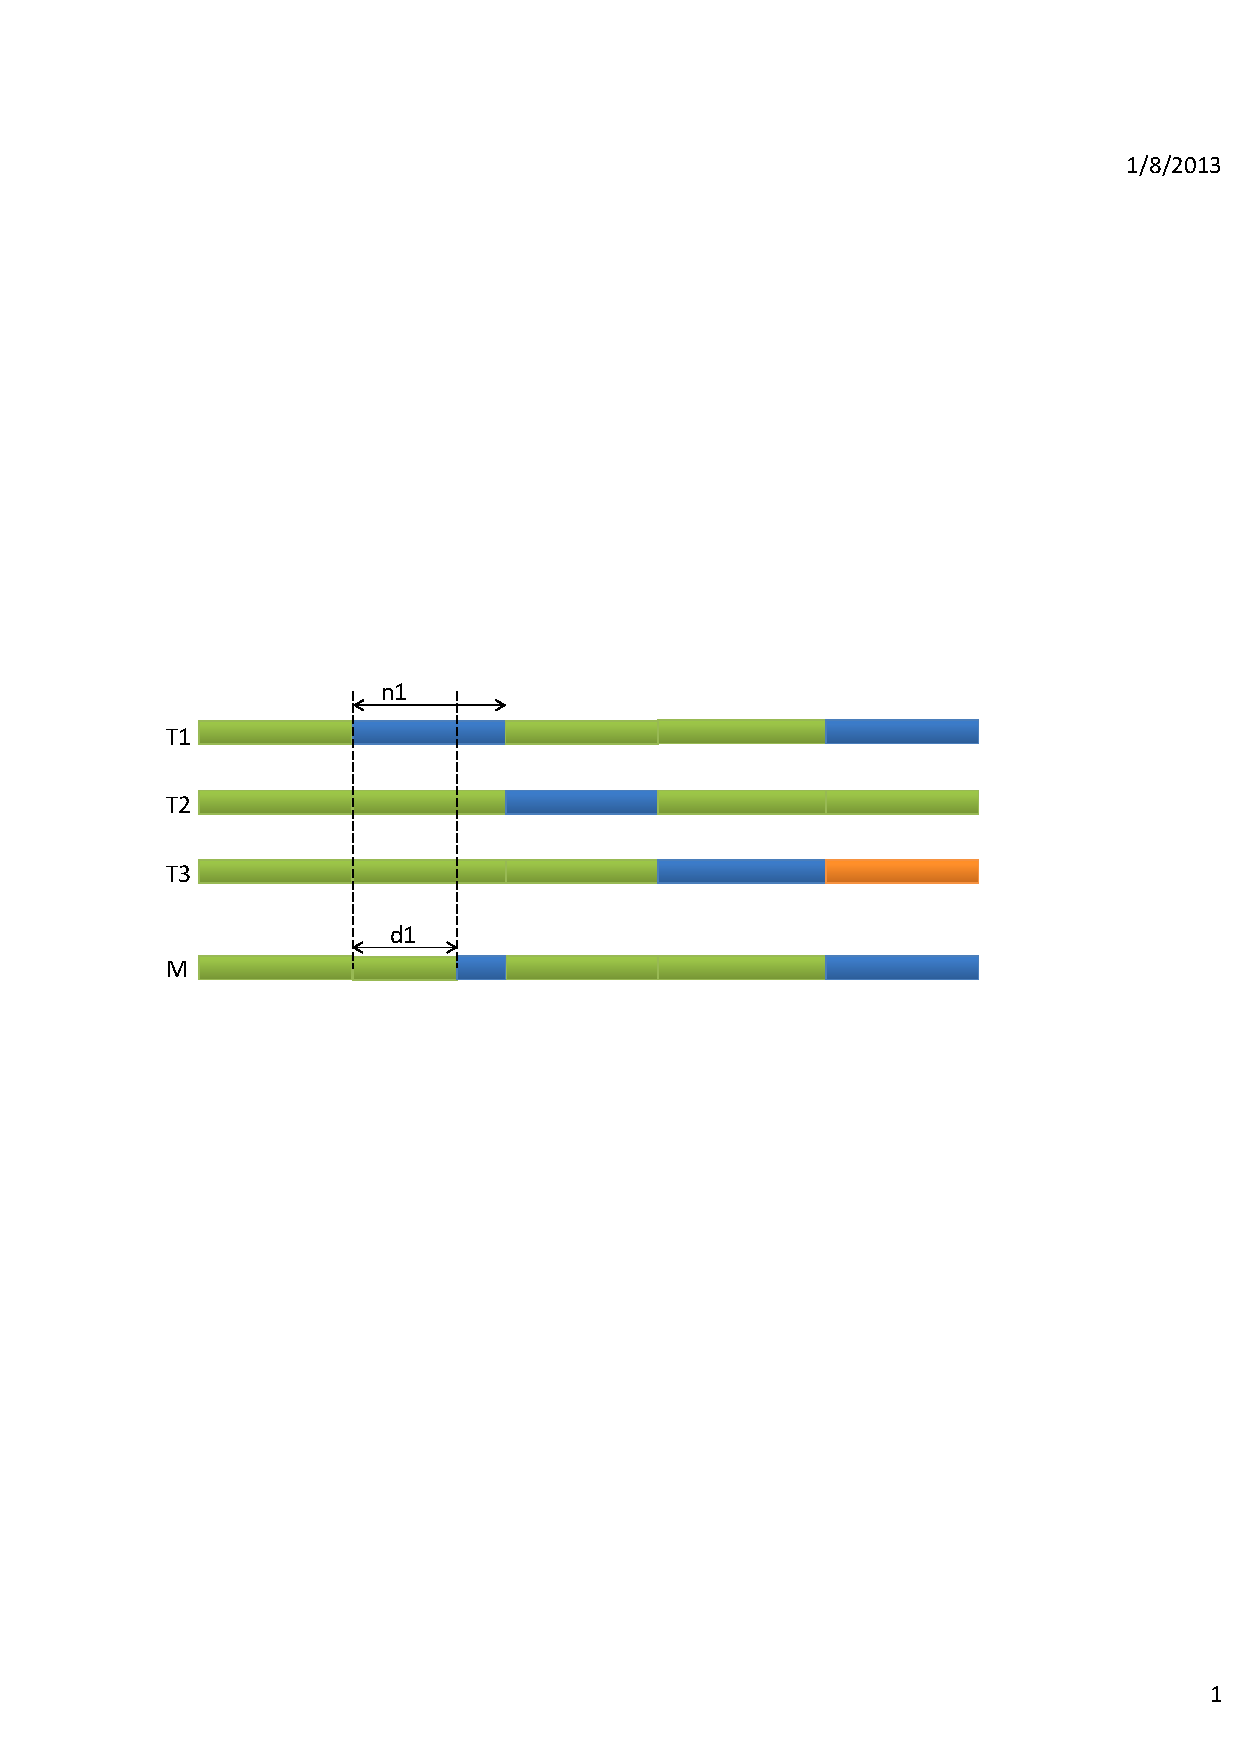
\includegraphics[width=\linewidth]{proof-case1}
Proof of theorem~\ref{th_3sufficient},  case 1:  There exists $i, 1 \leq i \leq 3$ for which $n_i\geq d_i$.
Without loss of generality we assume $i=1$.
The top 3 rows represent the input $l$-mers. The last row shows a common neighbor $M$. In any
column, identical colors represents matches, different colors represent mismatches.
\end{figure}

Case 2) For all $i, 1 \leq i \leq 3$ we have $n_i < d_i$. We construct $M$ as
shown in figure~\ref{figProofCase2}. For columns $k$ of type $N_0,N_2$ and $N_3$
we set $M[k]=t_1[k]$. For columns of type $N_1$ we set $M[k]=t_2[k]$.
For any $i,1\leq i \leq 3$ the following applies. If $n_i+n_4\leq d_i$ then the
Hamming distance between $M$ and $t_i$ is less than $d_i$ regardless of what
characters we choose for $M$ in the columns of type $N_4$.
On the other hand, if $n_i+n_4 > d_i$ then $M$ and $t_i$ have to match in at
least $n_i+n_4-d_i$ columns of type $N_4$. Thus, we pick
$max(0,n_i+n_4-d_i)$ columns of type $N_4$ and for each such column $k$ we set
$M[k]=t_i[k]$.
Now we prove that we actually have enough columns to make the
above choices, in other words $\Sigma_{i=1}^3max(0,n_i+n_4-d_i)\leq n_4$. This is equivalent to the following
conditions being true:
\begin{description}
\item[a)] For any $i, 1\leq i \leq 3$ we want $n_i+n_4-d_i \leq n_4$. This is
true because $n_i < d_i$.
\item[b)] For any $i,j, 1\leq i < j \leq 3$ we want
$(n_i+n_4-d_i)+(n_j+n_4-d_j) \leq n_4$. This can be rewritten as
$n_i+n_j+n_4\leq d_i+d_j$. The left hand side is $Hd(t_i, t_j)$ which
we know is less or equal to $d_i+d_j$.
\item[c)] We want $\Sigma_{i=1}^3n_i+n_4-d_i \leq n_4$. This can be rewritten as
$n_1 + n_2 + n_3 + 2 n_4 \leq d_1+d_2+d_3$. The left hand side is $Cd(T)$ which
we know is less than $d_1+d_2+d_3$.
\end{description}


\begin{figure}[!h]
\caption{Proof of theorem~\ref{th_3sufficient},
case 2}\label{figProofCase2}
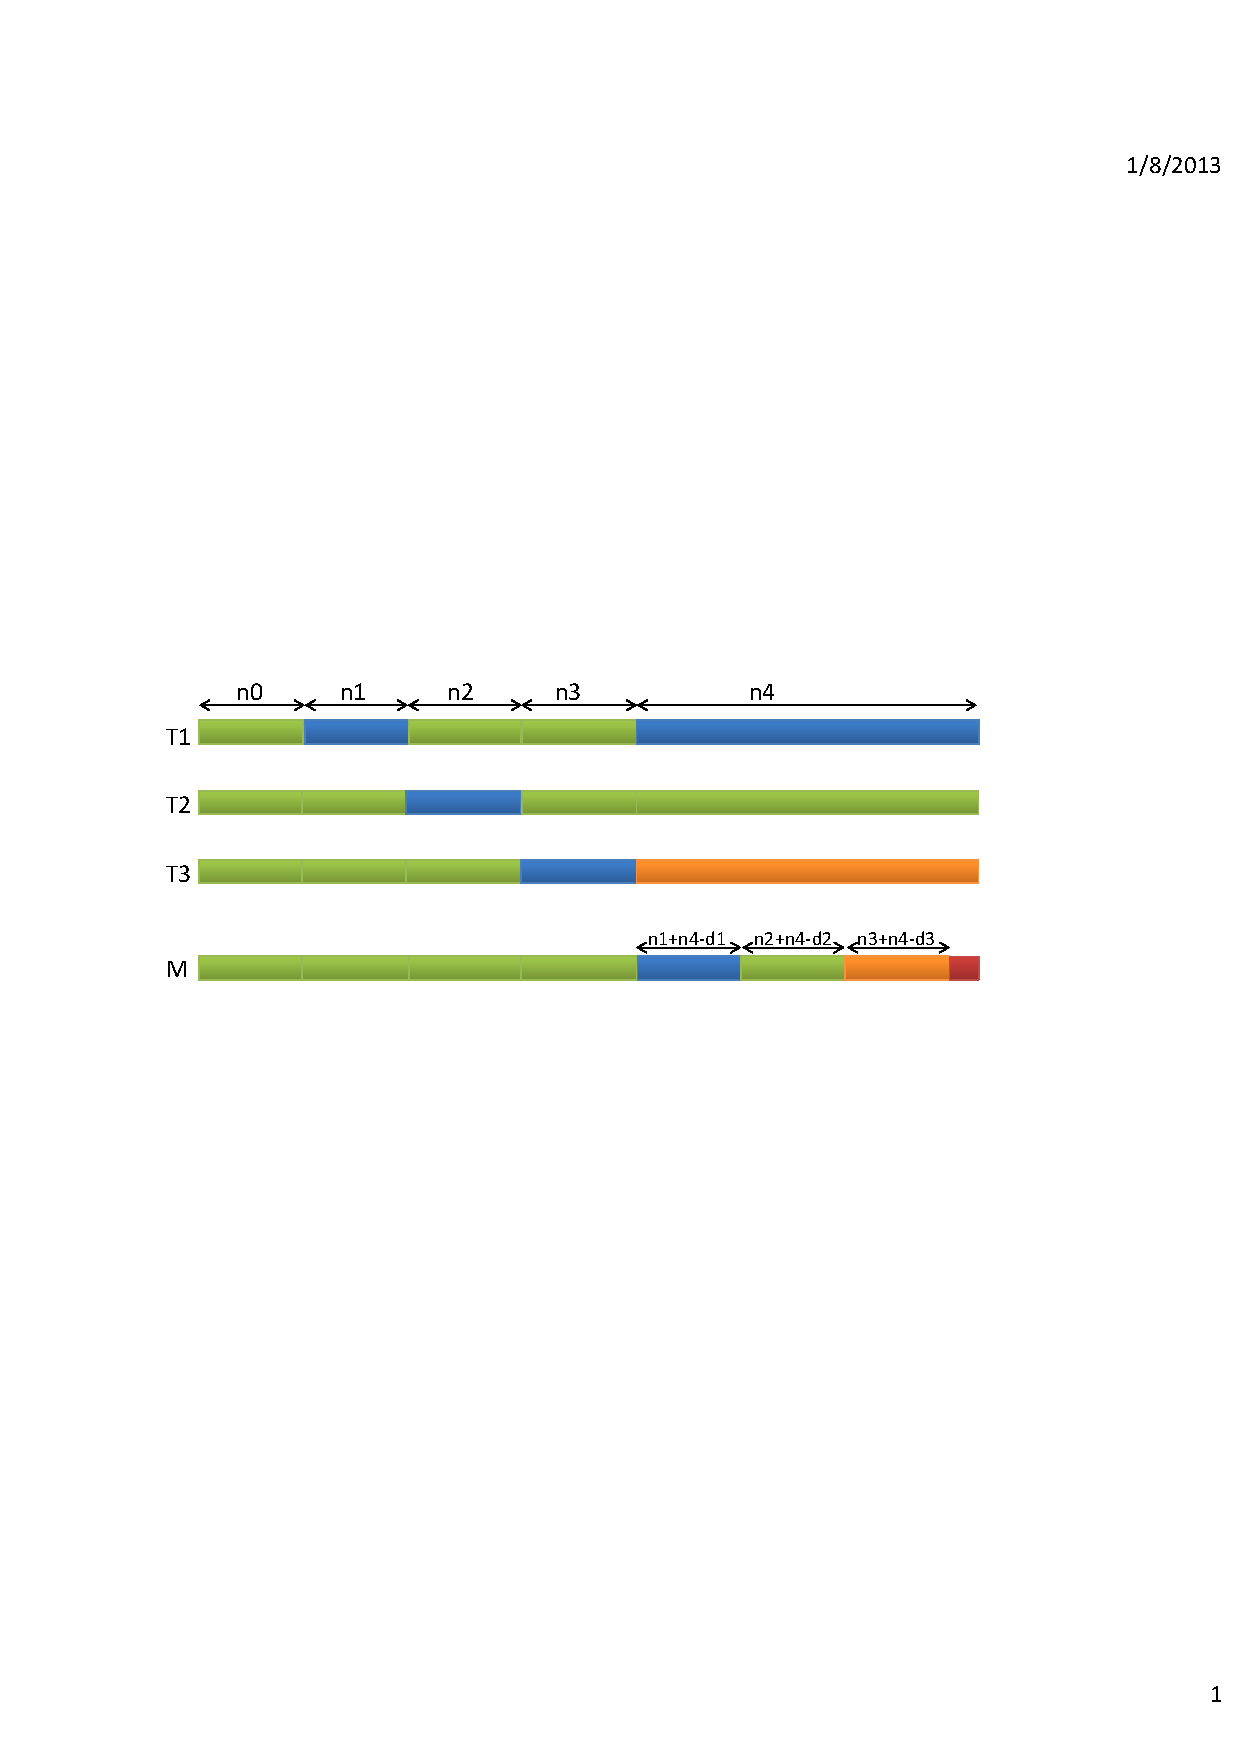
\includegraphics[width=\linewidth]{proof-case2}
Proof of theorem~\ref{th_3sufficient},
case 2: $n_i<d_i$ for all $i$, $1\leq i \leq 3$.
The top 3 rows represent the input $l$-mers. The last row shows a common neighbor $M$. In any
column, identical colors represents matches, different colors represent mismatches.
\end{figure}
\end{proof}



One of our reviewers kindly pointed out that the above proof is similar to an
algorithm in \cite{GNR01}.

\subsection{Adding Quorum Support}
In this section we extend the above techniques to solve the qPMS
problem. In the qPMS problem, when we generate tuples of $\ell$-mer, we may
``skip'' some of the strings.
This translates to the implementation as follows: in the PMS version we
successively try every alive $\ell$-mer in a given string by adding it to
the tuple $T$ and recursively calling the algorithm for the remaining strings.
For the qPMS version we have an additional step where, if the value of $q$
permits, we skip the current string and try $\ell$-mers
from the next string. At all times we keep track of how many strings we have
skipped. The pseudocode is given in algorithm \ref{figAlgQGenTuples}.
We invoke the algorithm as $QGenerateTuples(n-Q+1, \{\}, 0, k, R)$
where $Q=\lfloor\frac{qn}{100}\rfloor$ and $R$ contains all the $\ell$-mers in
all the strings.

\commentOut{
\begin{figure}
    \centering
    \includegraphics[width=1.0\textwidth]{algQGenTuples}
    \caption{This pseudocode generates tuples of $\ell$-mers that can potentially 
    have common neighbors, for the qPMS problem.\label{figAlgQGenTuples}}
\end{figure}
}

\begin{algorithm}
\SetKwInOut{Input}{Input}
\SetKwFunction{QGenerateTuples}{QGenerateTuples}
\SetKwFunction{ConsTotalDist}{Cd}
\SetKwFunction{GenerateNeighborhood}{GenerateNeighborhood}
\SetKwFunction{continue}{continue}

\caption{QGenerateTuples$(qTolerance,T,k,R)$} \label{figAlgQGenTuples}
\Input{$qTolerance$, number of strings we can afford to skip\;
\Indp\Indp $T=(t_1,t_2,\ldots,t_i)$, current tuple of $\ell$-mers\;
           $i$, last string processed\;
           $k$, desired size of the tuple\; 
           $R=(R_1, \ldots R_{n-i})$, where $R_j$ contains
           all alive $\ell$-mers in $s_{i+j}$\; 
}
\KwResult{Generates tuples of size $k$, containing $\ell$-mers, that have
common neighbors, then passes these tuples to the $\GenerateNeighborhood$
function\;}


\Begin{
\If {$|T|==k$}{
$\GenerateNeighborhood(T,d)$\;
\Return\;
}
outerLoop: \For {$u\in R_1$}{
$T':=T\cup \{u\}$\;
$incompat:=0$\; 
\For{$j \leftarrow 1$ \KwTo $n-i-1$}{
$R'_{j}=\{v \in R_{j+1} | \exists\; \text{common $d$-neighborhood for}\; T' \cup
\{v\}\}$\;
\If {$|R'_j|==0$} {
\If{$incompat \geq qTolerance$} {
\continue outerLoop\;
}
$incompat++$\;
}
$minAdd:=\min_{v \in R'_{j}} \ConsTotalDist(T'\cup \{v\}) -
\ConsTotalDist(T')$\; 
$aliveLmers:=|s_{i+j+1}|-|R'_{j}|$\; 
$sortKey[j]:= (minAdd, -aliveLmers)$ 
}
sort $R'$ decreasingly by $sortKey$\;
\QGenerateTuples$(qTolerance-incompat, T', k, R')$\;
}
\If{$qTolerance > 0$}{
\QGenerateTuples$(qTolerance-1, T, k, R \setminus R_1)$\;
}
}
\end{algorithm}


\subsection{Parallel Algorithm}

PMS8 and qPMS9 are parallel algorithms. Processor $0$ acts as both a master and
a worker, the other processors are workers. Each worker requests a subproblem from the
master, solves it, then repeats until all subproblems have been solved.
Communication between processors is done using the Message Passing Interface
(MPI). 

In PMS8, the subproblems are generated as follows. The search
space is split into $m=|s_1|-\ell+1$ independent subproblems $P_1, P_2,\ldots,
P_m$, where $P_i$ explores the $d$-neighborhood of $\ell$-mer $s_1[i..i+\ell-1]$.

In qPMS9, we extend the previous idea to the $q$ version. We split the
problem into subproblems $P_{1,1}, P_{1,2}, \ldots, P_{1,|s_1|-\ell+1}$,
$P_{2,1}, P_{2,2}, \ldots, P_{2,|s_2|-\ell+1}$, $\ldots$, $P_{r,1},
P_{r,2},\ldots,P_{r,|s_r|-\ell+1}$ where $r=n-Q+1$ and
$Q=\lfloor\frac{qn}{100}\rfloor$.
Problem $P_{i,j}$ explores the $d$-neighborhood of the $j$-th $\ell$-mer in string 
$s_i$ and searches for $\ell$-mers $M$ such that there are $Q-1$
instances of $M$ in strings $s_{i+1},\ldots,s_n$. Notice that $Q$ is
fixed, therefore subproblems $P_{i,j}$ get progressively easier as $i$
increases.


\subsection{Speedup Techniques}

\subsubsection{Speed up Hamming Distance calculation by packing $\ell$-mers}
\label{secCompressLmers}
By packing $\ell$-mers in advance we can speed up Hamming distance
operations. For example, we can pack 8 DNA characters in a 16 bit integer.
To compute the Hamming distance between two $l$-mers we first
perform an exclusive or of their packed representations. Equal
characters produce groups of zero bits, different characters produce
non-zero groups of bits.
For every possible $16$ bit integer $i$ we precompute the number of non-zero groups of bits
in $i$ and store it in a table. Therefore, one table look up provides the
Hamming distance for 8 DNA characters.  The same
technique applies to any alphabet $\Sigma$ besides DNA.

For an alphabet $\Sigma$ let $b=\lceil \log|\Sigma| \rceil$ be the number of
bits required to encode one character. Then, one compressed $\ell$-mer
requires $\ell * b$ bits of storage. However, due to
the overlapping nature of the $\ell$-mers in our input strings, we can employ
the following trick. In a 16 bit integer we can pack $p=\lfloor 16/b \rfloor$
characters. For every $\ell$-mer we only store the bit representation of its
first $p$ characters. The bit representation of the next $p$ characters is the
same as the bit representation of the first $p$ characters of the $l$-mer $p$ 
positions to the right of the current one. Therefore, the table of compressed
$l$-mers requires constant memory per $\ell$-mer, for a total of $O(n(m-l+1))$
words of memory.

\subsubsection{Preprocess Hamming distances for all pairs of input $\ell$-mers}
\label{secDistPairs}
The filtering step tests many times if two $l$-mers have a
distance of no more than $2d$. Thus, for every pair
of $l$-mers we preprocess this boolean information, provided the
required storage memory is not too high.

\subsubsection{Find motifs for a subset of the strings}
\label{secSubsetMotifs}
We also use the speedup technique described in \cite{RD11}: compute the motifs
for $n' < n$ of the input strings, then test each motif to see where it appears
in the remaining $n-n'$ strings. 

\subsubsection{Cache locality}
We can update $R$ in an efficient manner as follows. Every row in the
updated matrix $R'$ is a subset of the corresponding row in the current matrix
$R$, because some elements will be filtered out. Therefore, we can store $R'$
in the same memory locations as $R$. To do this, in each row, we move the elements belonging
to $R'$ at the beginning of the row and keep track of how many elements
belong to $R'$. To go from $R'$ back to $R$, we just have to restore the row
sizes to their previous values. The row elements will be the same even if they have
been permuted within the row. The same process can be repeated at every
step of the recursion, therefore the whole ``stack'' of $R$ matrices is stored in a
single matrix. This reduces the memory requirement and improves cache locality.
The cache locality is improved because at every step of the
recursion, in each row, we access a subset of the elements we accessed in the previous step, and
those elements are in contiguous locations of memory.


\subsection{Memory and Runtime}
Since we store all matrices $R$ in the space of a single matrix they
only require $O(n(m-l+1))$ words of memory. To this we add $O(n^2)$ words to store
 row sizes for the at most $n$ matrices which share the same space.
 The bits of information for $l$-mer pairs that have Hamming distance no
 more than $2d$ require $O((n(m-l+1))^2/w)$ words, where $w$ is the number of
 bits in a machine word.
The table of compressed $l$-mers takes $O(n(m-l+1))$ words. Therefore, the
total memory used by the algorithm is $O(n(n+m-l+1) + (n(m-l+1))^2 / w)$.

\subsection{Expected Number of Spurious Motifs}

It is useful to estimate how many ``spurious'' motifs (motifs expected by random
chance) will be found in a random sample. For that, we make the following
observations. The probability that a random $\ell$-mer $u$ is within distance
at most $d$ from another $\ell$-mer $v$ is

\begin{align}
p(\ell,d,\Sigma)=\frac{\sum_{i=0}^d\left(^\ell_i\right)(|\Sigma|-1)^i}{\Sigma^\ell}
\end{align}

The probability that an $\ell$-mer is within distance $d$ from any of the
$\ell$-mers in a string $S$ of length $m$ is: 

\begin{align}
P(m, \ell, d, \Sigma) = 1-(1-p(\ell,d,\Sigma))^{m-\ell+1}
\end{align}

The probability that an $\ell$-mer is within distance $d$ from at least
$q$ out of $n$ strings of length $m$ each is:

\begin{align}
Q(q,n,m,\ell,d,\Sigma)=\sum_{i=q}^n\left(^n_i\right)P(m,\ell,d,\Sigma)^i(1-P(m,\ell,d,\Sigma))^{n-i}
\end{align}

Therefore, the expected number of motifs for a given qPMS instance is:
$|\Sigma|^\ell Q(q,n,m,\ell,\Sigma)$. Based on
these formulas, we compute for every $\ell$ the largest value of $d$
such that the number of spurious motifs does not exceed 500. This gives us
the challenging instance for any $l$. These values are presented in table
\ref{maxdDNA} for DNA and table \ref{maxdProtein} for protein.

\section{Results}
\label{sec_pms_results}


As mentioned in the introduction, PMS algorithms are typically tested on
datasets generated as follows. 20 strings of length 600 each are generated from
the i.i.d. We choose an
$\ell$-mer $M$ as a motif and plant modified versions of it in $q\%$ of the
$n$ strings. Each planted instance is modified in $d$ random positions.
For every $(l,d)$ combination we generate 5 random datasets and report the
average runtime over all 5.

Programs were executed on the Hornet cluster at the University of Connecticut, 
which is a high-end, 104-node, 1408-core High Performance Computing cluster. 
For our experiments we used Intel Xeon X5650 Westmere cores. Results refer to
single core execution, unless specified otherwise.

\subsection{PMS8}
In this section we analyze the performance of PMS8 \cite{NRPMS14}.
The speedup obtained by the parallel version over the single core version,
for several challenging instances, is presented in figure~\ref{PMS8figSpeedup}.
The speedup for $p=48$ cores is close to $S=45$ and thus the
efficiency is $E=S/p=94\%$.

\begin{figure}
\caption{PMS8: Speedup of the multi-core version over the single core
version, for several datasets.}\label{PMS8figSpeedup} 
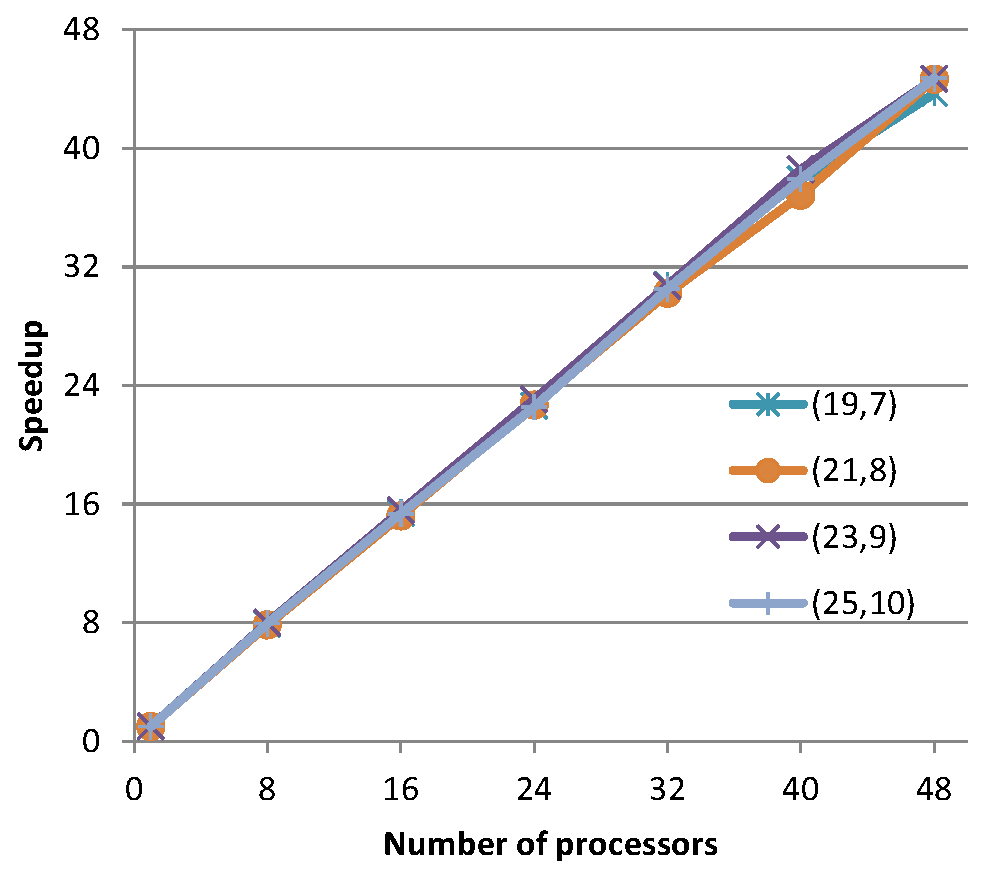
\includegraphics[width=\linewidth]{PMS8speedup}
\end{figure}

The runtime of PMS8 on instances with $l$ up to $50$ and $d$ up
to $21$ is shown in figure~\ref{PMS8figLDTable}. Instances which are expected to
have more than $500$ motifs simply by random chance (spurious motifs) are excluded.
Instances where $d$ is small relative to $l$ are solved using a single CPU core.
For more challenging instances we report the time taken using 48 cores.

\begin{figure}
\caption{PMS8: Runtimes for datasets with $l$ up to 50 and $d$ up to
25.}\label{PMS8figLDTable}
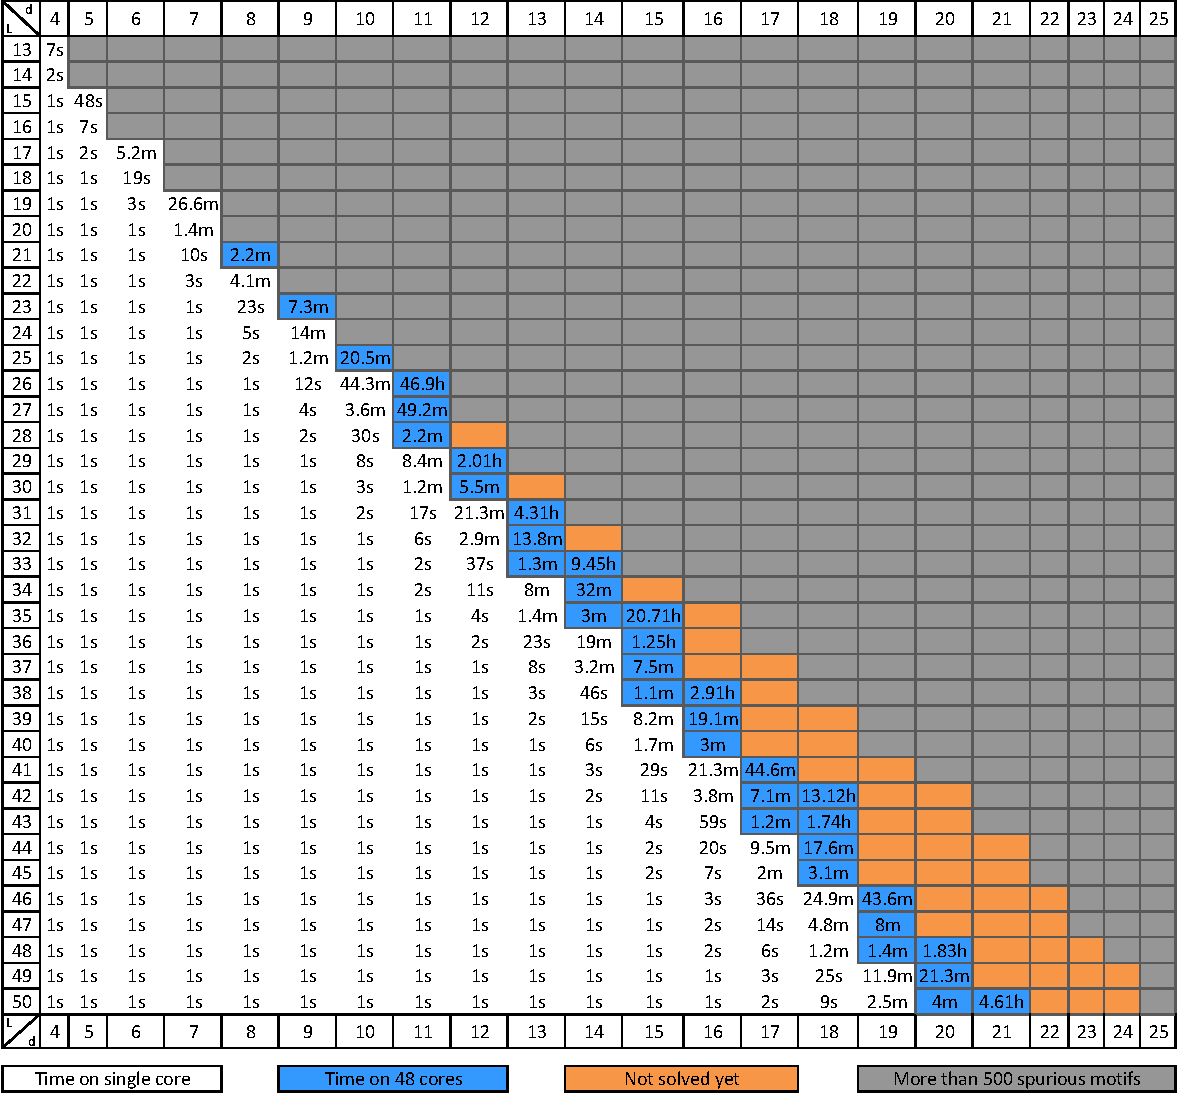
\includegraphics[width=1\linewidth]{PMS8dnaruntimes}
 All runtimes are averages over 5 random datasets.
 White background signifies single
core execution.  Blue background signifies execution using 48 cores.
Instances in gray have more than 500 spurious motifs. Orange
cells indicate unsolved instances. Time is reported in hours (h), minutes (m)
and seconds (s).
\end{figure}

A comparison between PMS8 and qPMS7 \cite{DRD12} on
challenging instances is shown in table~\ref{PMS8figCompChallenging}.
qPMS7 is a sequential algorithm. PMS8 was evaluated using up to 48 cores.
The speedup of PMS8 single core over qPMS7
is shown in figure~\ref{PMS8figSpeedupQPMS7}. The speedup is high for small
instances because qPMS7 has to load an ILP table. 
For larger instances the speedup of PMS8 sharply increases. This is expected
because qPMS7 always generates neighborhoods for tuples of $3$ $l$-mers, 
which become very large as $l$ and $d$ grow. On the other hand, PMS8 increases
the number of $l$-mers in the tuple with the instance size. 
 The peak memory used by qPMS7 for the challenging instances in
 table~\ref{PMS8figCompChallenging} was 607 MB whereas for PMS8 it was 122 MB.
 PMS8 was the first algorithm to solve the challenging instance (26,11).


\begin{table}
\caption{
 Comparison between qPMS7 and PMS8 on challenging instances. 
}\label{PMS8figCompChallenging}
\begin{tabular}{cccccc@{\extracolsep\fill}}
\hline
\textbf{Instance} & \textbf{qPMS7} & \textbf{PMS8$^1$} & \textbf{PMS8$^{16}$} &
\textbf{PMS8$^{32}$} & \textbf{PMS8$^{48}$} \\
\hline
(13,4) & 29s     & 7s     & 3s    & 2s    & 2s \\
(15,5) & 2.1m    & 48s    & 5s    & 4s    & 3s \\
(17,6) & 10.3m   & 5.2m   & 22s   & 12s   & 9s \\
(19,7) & 54.6m   & 26.6m  & 1.7m  & 52s   & 37s \\
(21,8) & 4.87h   & 1.64h  & 6.5m  & 3.3m  & 2.2m \\
(23,9) & 27.09h  & 5.48h  & 21.1m & 10.7m & 7.4m \\
(25,10)& -       & 15.45h & 1.01h & 30.4m & 20.7m \\
(26,11)& -       & -      & -     & -     & 46.9h \\
\hline
\end{tabular}\\
 PMS$8^P$ means  
 PMS8 used $P$ CPU cores. Both programs have been executed on the same hardware 
 and the same datasets. The times are average runtimes over 5 instances for each 
 dataset.
\end{table}



\begin{figure}
\caption{Speedup of PMS8 single core over qPMS7.}\label{PMS8figSpeedupQPMS7}
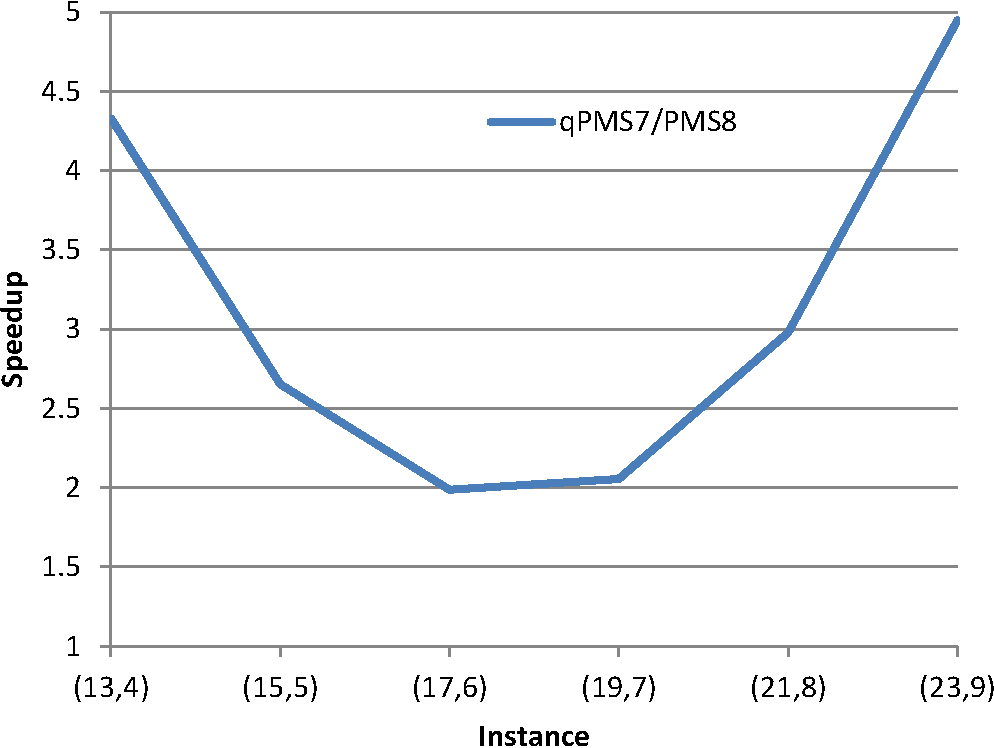
\includegraphics[width=\linewidth]{PMS8speedupQPMS7}
Ratio of runtimes between
qPMS7 and PMS8 running on a single core. Both programs have been executed on the same
hardware and the same datasets. The times are average runtimes over 5 instances
for each dataset.
\end{figure}


Some results in the literature have also focused on instances other than
the challenging ones presented above. A summary of these results and a comparison
with PMS8 is presented in table~\ref{pms8_table_comparison}. These results have been obtained on various types of hardware: single core,
multi-core, GPU, grid. In the comparison, we try to match the number of processors whenever possible.
The speed difference is of several orders of magnitude in some cases which indicates that
the pruning conditions employed by PMS8 significantly reduce the
search space compared to other algorithms.


\begin{table}

\caption{Comparison between PMS8 and contemporary
results in the literature.}\label{pms8_table_comparison}
\begin{tabular}{| p{2.5in} | p{0.5in} | p{0.5in} | p{0.6in} | p{0.4in} | p{0.4in} |}
\hline
Previous algorithm & Instance & Time & Cores & PMS8 Time & PMS8 Cores\\
\hline
Abbas et al. 2012 \cite{AAB12},  PHEP\_PMSprune & (21,8) & 20.42h & 8 & 6.5m & 1 \\
\hline
Yu et al. 2012 \cite{YHZG12}, PairMotif & (27, 9) & 10h & 1 & 4s & 1\\
\hline
\multirow{2}{*}{Desaraju and Mukkamala 2011 \cite{DeM11}} & (24,6) & 347s & 1 & 1s & 1\\
\cline{2-6}
                                         & (48,12)& 188s & 1 & 1s & 1\\
\hline
\multirow{2}{*}{\vbox{Dasari et al. 2011 \cite{DRZ11}, mSPELLER / gSPELLER}} & (21,8) & 3.7h & 16 & 6.5m & 16\\
\cline{2-6}
                                                   & (21,8) & 2.2h & \multirow{2}{*}{\vbox{4 GPUs x 240 cores}} & 6.5m & 16\\
\cline{1-3}\cline{5-6}
Dasari et al. 2010 \cite{DDZ10}, BitBased & (21,8) & 1.1h & & 6.5m & 16\\
\hline
Dasari and Desh 2010 \cite{DD10}, BitBased & (21,8) & 6.9h & 16 & 6.5m & 16\\
\hline
Sahoo et al. 2011 \cite{SSRP11} & (16,4) & 106s & 4 & 1s & 1\\
\hline
Sun et al. 2011 \cite{SLHTR11}, TreeMotif &(40,14) & 6h & 1 & 6s & 1\\
\hline
He et al. 2010 \cite{HLWR10}, ListMotif & (40,14) & 28,087s & 1 & 6s &1\\
\hline
Faheem 2010 \cite{Fah10}, skip-Brute Force & (15,4) & 2934s & 96 nodes & 1s & 1\\
\hline
\multirow{3}{*}{Ho et al. 2009 \cite{HJG09}, iTriplet} & (24,8) & 4h & 1 & 5s & 1\\
\cline{2-6}
                                      & (38,12) & 1h & 1 & 1s & 1\\
\cline{2-6}
                                      & (40,12) & 5m & 1 & 1s & 1\\
\hline
\end{tabular}\\
 Time is reported in seconds (s), minutes (m) 
or hours (h). Note that the hardware is different, though we tried to match
the number of processors when possible. Also, the instances are randomly
generated using the same algorithm, however the actual instances used by the
various papers are most likely different. For PMS8, the times are averages
over 5 randomly generated instances.
\end{table}



We compared PMS8 with qPMS7 on the real datasets discussed in
\cite{TLB+05}. We excluded datasets with less than $4$ input
sequences because these are not very challenging. For each dataset we chose two
combinations of $l$ and $d$. These combinations were chosen on a dataset
basis because for large values of $d$ the number of reported motifs is
excessive and for small values of $d$ the instance is not very challenging.
To make qPMS7 behave like PMS8 we set the quorum percent to $100\%$ ($q=n$).
The comparison is shown in table \ref{pms8_table_real_data}. Note that both algorithms
are exact algorithms and therefore the sensitivity and specificity are the same.


\begin{table}
\caption{Runtime comparison between PMS8 and qPMS7 on real datasets from
\cite{TLB+05}}\label{pms8_table_real_data}
\scalebox{0.96}{
\begin{tabular}{ccccccc@{\extracolsep\fill}}
\hline
\textbf{Dataset} & \textbf{n} & \textbf{Total no. bases} & \textbf{$\ell$} &
\textbf{d} & \textbf{PMS8 time} & \textbf{qPMS7 time}\\
\hline
dm01r & 4 & 6000 & 21 & 4 & 1 & 55 \\
dm01r & 4 & 6000 & 23 & 5 & 1 & 6 \\
dm04r & 4 & 8000 & 21 & 4 & 1 & 5 \\
dm04r & 4 & 8000 & 23 & 5 & 1 & 5 \\
\hline
hm01r & 18 & 36000 & 21 & 6 & 10 & 14 \\
hm01r & 18 & 36000 & 23 & 7 & 25 & 40 \\
hm02r & 9 & 9000 & 21 & 6 & 1 & 11 \\
hm02r & 9 & 9000 & 23 & 7 & 4 & 35 \\
hm03r & 10 & 15000 & 21 & 6 & 3 & 24 \\
hm03r & 10 & 15000 & 23 & 7 & 14 & 146 \\
hm04r & 13 & 26000 & 21 & 6 & 6 & 44 \\
hm04r & 13 & 26000 & 23 & 7 & 15 & 39 \\
hm05r & 3 & 3000 & 21 & 4 & 1 & 6 \\
hm05r & 3 & 3000 & 23 & 5 & 1 & 46 \\
hm08r & 15 & 7500 & 17 & 5 & 1 & 7 \\
hm08r & 15 & 7500 & 17 & 6 & 46 & 251 \\
hm19r & 5 & 2500 & 23 & 5 & 1 & 5 \\
hm19r & 5 & 2500 & 23 & 6 & 1 & 5 \\
hm20r & 35 & 70000 & 21 & 6 & 27 & 32 \\
hm20r & 35 & 70000 & 23 & 7 & 56 & 136 \\
hm26r & 9 & 9000 & 23 & 6 & 1 & 5 \\
hm26r & 9 & 9000 & 23 & 7 & 5 & 46 \\
\hline
mus02r & 9 & 9000 & 21 & 6 & 1 & 11 \\
mus02r & 9 & 9000 & 23 & 7 & 2 & 45 \\
mus04r & 7 & 7000 & 21 & 6 & 1 & 15 \\
mus04r & 7 & 7000 & 23 & 7 & 2 & 22 \\
mus05r & 4 & 2000 & 21 & 5 & 1 & 79 \\
mus05r & 4 & 2000 & 23 & 6 & 1 & 5 \\
mus07r & 4 & 6000 & 21 & 5 & 1 & 79 \\
mus07r & 4 & 6000 & 23 & 5 & 1 & 6 \\
mus10r & 13 & 13000 & 21 & 6 & 2 & 56 \\
mus10r & 13 & 13000 & 23 & 7 & 2 & 70 \\
mus11r & 12 & 6000 & 21 & 7 & 8 & 150 \\
mus11r & 12 & 6000 & 23 & 8 & 23 & 938 \\
\hline
yst01r & 9 & 9000 & 21 & 6 & 2 & 14 \\
yst01r & 9 & 9000 & 23 & 7 & 8 & 63 \\
yst02r & 4 & 2000 & 21 & 5 & 1 & 5 \\
yst02r & 4 & 2000 & 23 & 6 & 1 & 6 \\
yst03r & 8 & 4000 & 21 & 6 & 1 & 8 \\
yst03r & 8 & 4000 & 23 & 7 & 1 & 19 \\
yst04r & 6 & 6000 & 21 & 4 & 1 & 5 \\
yst04r & 6 & 6000 & 23 & 5 & 1 & 5 \\
yst05r & 3 & 1500 & 21 & 4 & 1 & 5 \\
yst05r & 3 & 1500 & 23 & 5 & 1 & 5 \\
yst06r & 7 & 3500 & 21 & 6 & 1 & 6 \\
yst06r & 7 & 3500 & 23 & 7 & 2 & 12 \\
yst08r & 11 & 11000 & 21 & 5 & 1 & 6 \\
yst08r & 11 & 11000 & 23 & 6 & 1 & 6 \\
yst09r & 16 & 16000 & 21 & 6 & 2 & 17 \\
yst09r & 16 & 16000 & 23 & 7 & 6 & 68 \\
\hline
\end{tabular}
}

For each dataset we tested two combinations of $l$ and $d$. For qPMS7 we set $q=n$. Both algorithms were executed on a single CPU core. Time is reported in seconds, rounded up to the next second.
\end{table}



\subsection{qPMS9}
In the previous section we have seen that PMS8 outperformed all of the
algorithms we could find in the literature at the time. After the
publication of PMS8, the TraverStringRef \cite{T14} algorithm came out.
Therefore, in this section we only compare PMS8, TraverStringRef and qPMS9. For
$q=100\%$ we compare all three algorithms, for $q=50\%$ we compare only the
algorithms that solve the quorum PMS problem: TraverStringRef and qPMS9.

For $q=100\%$, we compare the three algorithm on DNA data 
in table \ref{timePmsDna}. A similar comparison on protein data is given in
table \ref{timePmsProtein}.

For $q=50\%$, we compare TraverStringRef and
qPMS9 on DNA data in table \ref{timePmsDNAq50}. A similar comparison on protein
data is given in \ref{timePmsProteinq50}.

The running time of qPMS9 on DNA datasets for all combinations of $\ell$ and $d$
with $\ell$ up to 50 and $d$ up to 25, with $q=100\%$, is given in Figure
\ref{figDnaRuntimes}. The running time of qPMS9 on
protein datasets for all combinations of $\ell$ and $d$ with $\ell$ up to 30 and
$d$ up to 21, with $q=100\%$, is given in Figure \ref{figProteinRuntimes}.

\begin{figure}
    \caption{qPMS9 runtimes on DNA datasets for multiple combinations of $\ell$
    and $d$ where $q=100\%$. 
    \label{figDnaRuntimes}}
    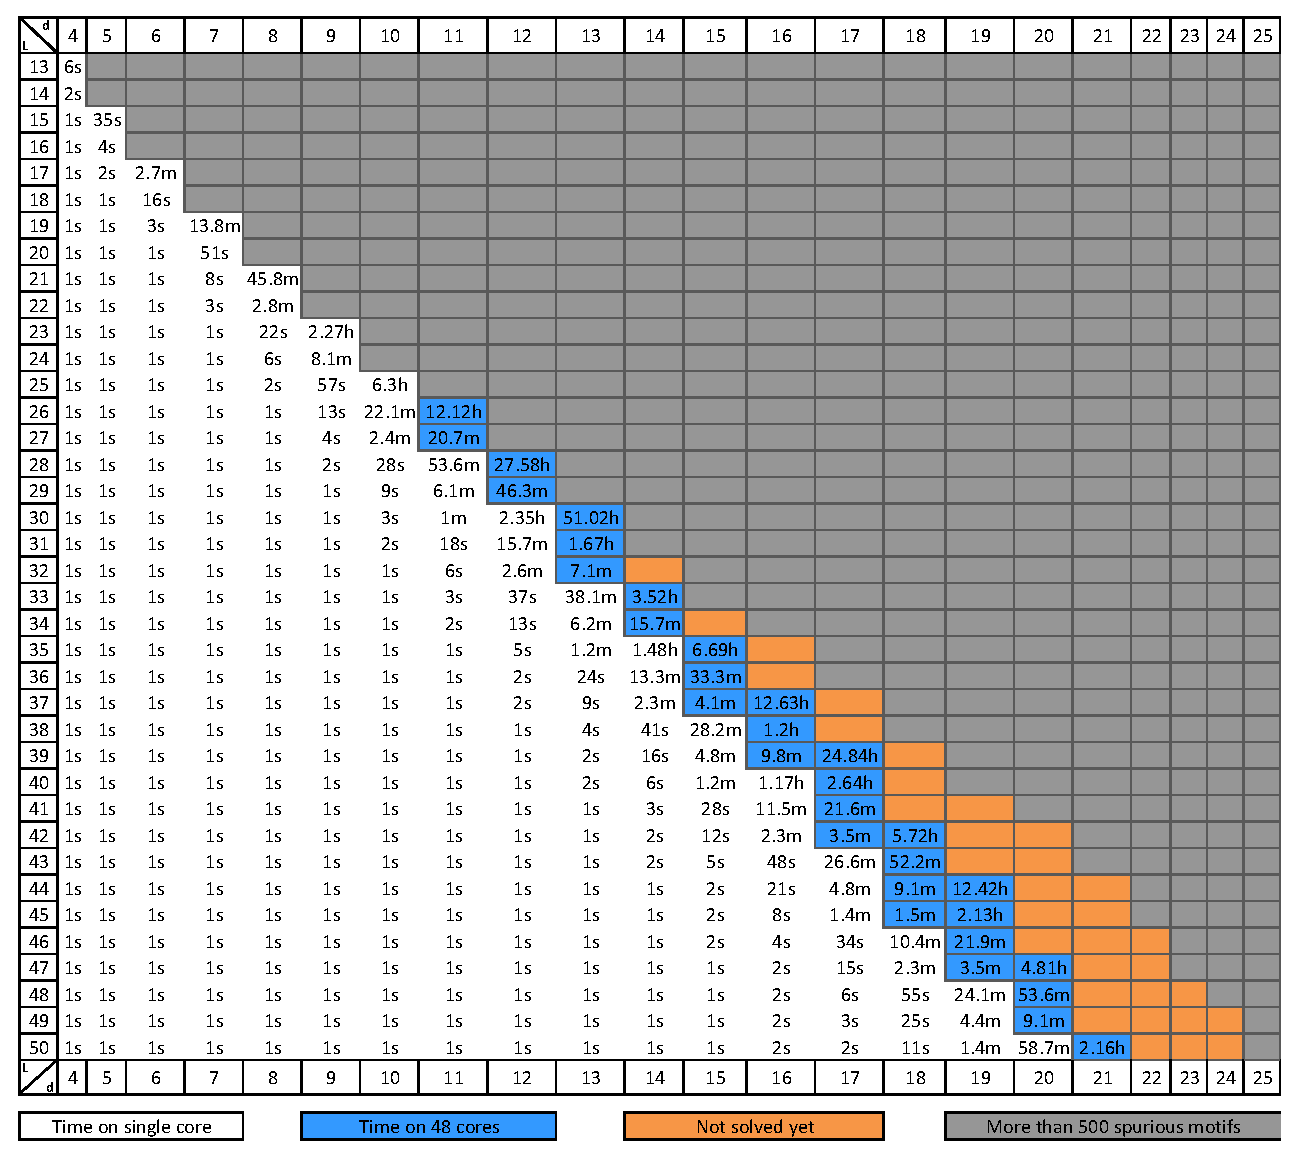
\includegraphics[width=1.0\textwidth]{qpms9-dna-runtimes}
    The runtimes are averages over 5 random datasets. The
    times are given in hours (h) minutes (m) or seconds (s). Grey cells indicate instances that
    are expected to have more than 500 motifs by random chance (spurious
    motifs). Blue cells indicate that the program used 48 cores whereas white
    cells indicate single core execution. Instances in orange could not be
    solved efficiently.
\end{figure}

\begin{figure}
    \caption{qPMS9 runtimes on protein datasets for multiple combinations
    of $\ell$ and $d$ where $q=100\%$. }\label{figProteinRuntimes}
    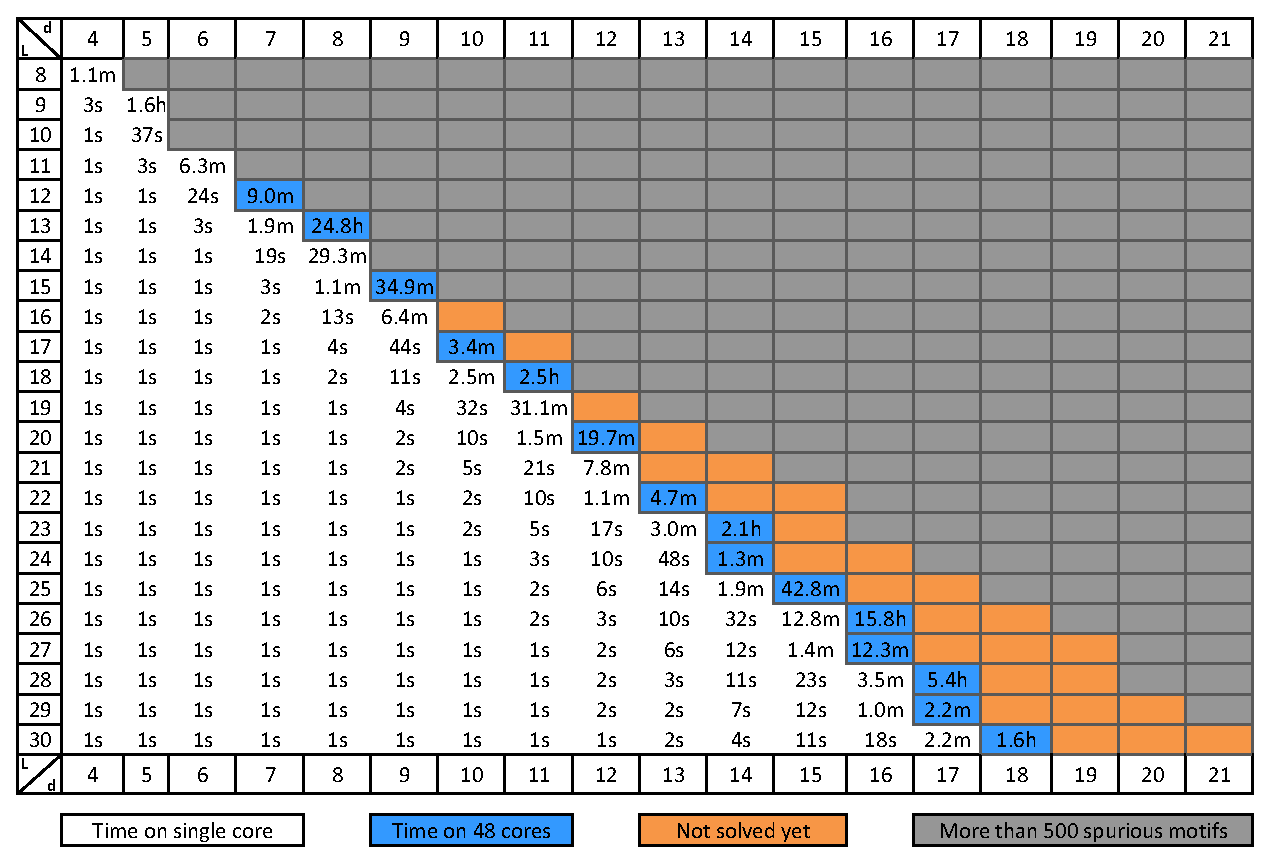
\includegraphics[width=1.0\textwidth]{qpms9-protein-runtimes}
    The runtimes are averages over 5 random
    datasets. The times are given in hours (h) minutes (m) or seconds (s). 
    Grey cells indicate instances that
    are expected to have more than 500 motifs by random chance (spurious
    motifs). Blue cells indicate that the program used 48 cores whereas white
    cells indicate single core execution. Instances in orange could not be
    solved efficiently.
\end{figure}

\begin{table}
\caption{Maximum value of $d$ such
that the expected number of spurious motifs in random datasets does not exceed
$500$, for $\ell$ up to 50 and $q$ between $50\%$ and $100\%$, on DNA data.}\label{maxdDNA}
\begin{tabular}{| c | c | c | c |}
\hline
 & \multicolumn{3}{| c |}{max d}\\
\hline
L & $q=50\%$ & $q=75\%$ & $q=100\%$\\
\hline
13 & 3 & 3 & 4\\
14 & 3 & 4 & 4\\
15 & 4 & 4 & 5\\
16 & 4 & 5 & 5\\
17 & 4 & 5 & 6\\
18 & 5 & 6 & 6\\
19 & 5 & 6 & 7\\
20 & 6 & 7 & 7\\
21 & 6 & 7 & 8\\
22 & 7 & 8 & 8\\
23 & 7 & 8 & 9\\
24 & 8 & 9 & 9\\
25 & 8 & 9 & 10\\
26 & 9 & 10 & 11\\
27 & 9 & 10 & 11\\
28 & 10 & 11 & 12\\
29 & 10 & 11 & 12\\
30 & 11 & 12 & 13\\
31 & 11 & 12 & 13\\
32 & 12 & 13 & 14\\
33 & 12 & 13 & 14\\
34 & 13 & 14 & 15\\
35 & 13 & 15 & 16\\
36 & 14 & 15 & 16\\
37 & 14 & 16 & 17\\
38 & 15 & 16 & 17\\
39 & 15 & 17 & 18\\
40 & 16 & 17 & 18\\
41 & 16 & 18 & 19\\
42 & 17 & 18 & 20\\
43 & 17 & 19 & 20\\
44 & 18 & 19 & 21\\
45 & 18 & 20 & 21\\
46 & 19 & 21 & 22\\
47 & 19 & 21 & 22\\
48 & 20 & 22 & 23\\
49 & 20 & 22 & 24\\
50 & 21 & 23 & 24\\
\hline
\end{tabular}
\end{table}

\begin{table}
\caption{
Maximum value of $d$ such
that the expected number of spurious motifs in random datasets does not exceed
$500$, for $\ell$ up to 30 and $q$ between $50\%$ and $100\%$, on protein data.
}\label{maxdProtein}
\begin{tabular}{| c | c | c | c |}
\hline
 & \multicolumn{3}{| c |}{max d}\\
\hline
L & $q=50\%$  & $q=75\%$ & $q=100\%$ \\
\hline
9 & 4 & 4 & 5\\
10 & 4 & 5 & 5\\
11 & 5 & 6 & 6\\
12 & 6 & 6 & 7\\
13 & 6 & 7 & 8\\
14 & 7 & 8 & 8\\
15 & 8 & 9 & 9\\
16 & 9 & 9 & 10\\
17 & 9 & 10 & 11\\
18 & 10 & 11 & 11\\
19 & 11 & 12 & 12\\
20 & 11 & 12 & 13\\
21 & 12 & 13 & 14\\
22 & 13 & 14 & 15\\
23 & 14 & 15 & 15\\
24 & 14 & 15 & 16\\
25 & 15 & 16 & 17\\
26 & 16 & 17 & 18\\
27 & 16 & 18 & 19\\
28 & 17 & 18 & 19\\
29 & 18 & 19 & 20\\
30 & 19 & 20 & 21\\
\hline
\end{tabular}
\end{table}

\begin{table}
\caption{PMS runtimes for DNA data when $q=100\%$.}\label{timePmsDna}
\begin{tabular}{| c | c | c | c |}
\hline
$(\ell,d)$ & TraverStringRef & PMS8 &  qPMS9\\
\hline
(13,4) & 14s & 7s &  \textbf{6s}\\
\hline
(15,5) & 55s & 48s & \textbf{34s}\\
\hline
(17,6) & 3.5m & 5.2m & \textbf{2.7m}\\
\hline
(19,7) & 14.5m & 26.6m & \textbf{13.4m}\\
\hline
(21,8) & 59.8m & 1.64h & \textbf{45.4m}\\
\hline
(23,9) & 4.08h & 5.48h & \textbf{2.26h}\\
\hline
(25,10) & 17.55h & 15.45h & \textbf{6.3h}\\
\hline
\end{tabular}\\
 The time is given in
hours (h), minutes (m) or seconds (s), averaged over 5
datasets.
\end{table}

\begin{table}
\caption{PMS runtimes for protein data when $q=100\%$.}
\label{timePmsProtein}
\begin{tabular}{| c | c | c | c |}
\hline
$(\ell,d)$ & TraverStringRef & PMS8 & qPMS9\\
\hline
(10,5) & 2.6m & 42s & \textbf{37s}\\
\hline
(11,6) & 1.67h & 11m & \textbf{6.1m}\\
\hline
(13,7) & 58.2m & 2.6m & \textbf{19s}\\
\hline
(14,8) & TL & 1.03h & \textbf{29.6m}\\
\hline
(15,8) & 28.5m & 1.2m & \textbf{1.1m}\\
\hline
(17,9) & 16.6m & 45s & \textbf{43s}\\
\hline
(19,10) & 5.9m & \textbf{32s} & \textbf{32s}\\
\hline
(19,11) & TL & 1.23h & \textbf{30.1m}\\
\hline
(22,12) & 3.73h & 1.2m & \textbf{1.1m}\\
\hline
(24,13) & 1.84h & 48s & \textbf{47s}\\
\hline
(26,14) & 30.7m & \textbf{31s} & 32s\\
\hline
(26,15) & TL & 1.19h & \textbf{12.5m}\\
\hline
\end{tabular}\\
 The time is given in
hours (h), minutes (m) or seconds (s), averaged over 5
datasets. TL means that the program runs for more than 24h.
\end{table}


\begin{table}
\caption{
PMS runtimes for DNA data when $q=50\%$.}\label{timePmsDNAq50}
\begin{tabular}{| c | l | l |}
\hline
Instance & TraverStringRef & qPMS9\\
\hline
(20,6) & 3m & \textbf{1.5m}\\
\hline
(22,7) & 12.9m & \textbf{6.3m}\\
\hline
(23,7) & 2.6m & \textbf{48s}\\
\hline
(24,8) & 56m & \textbf{26.3m}\\
\hline
(25,8) & 9.9m & \textbf{3.1m}\\
\hline
(26,9) & 4.31h & \textbf{1.55h}\\
\hline
(27,9) & 39.9m & \textbf{10.6m}\\
\hline
(28,10) & 20.86h & \textbf{5.15h}\\
\hline
(29,10) & 2.89h & \textbf{34.5m}\\
\hline
\end{tabular}\\
 The time is given in
hours (h), minutes (m) or seconds (s), averaged over 5
datasets.
\end{table}


\begin{table}
\caption{
PMS runtimes for protein data when $q=50\%$.}
\label{timePmsProteinq50}
\begin{tabular}{| c | c | c | c |}
\hline
Instance & TraverStringRef & qPMS9\\
\hline
(9,4) & 11.3m & \textbf{3.7m}\\
\hline
(11,5) & 14m & \textbf{4.1m}\\
\hline
(12,6) & 6.22h & \textbf{57.5m}\\
\hline
(13,6) & 17.4m & \textbf{4.9m}\\
\hline
(14,7) & 5.09h & \textbf{41.3m}\\
\hline
(15,8) & TL & \textbf{4.62h}\\
\hline
(17,9) & TL & \textbf{1.79h}\\
\hline
(18,9) & 2.71h & \textbf{33.1m}\\
\hline
(20,10) & 2.33h & \textbf{33.3m}\\
\hline
(21,11) & TL & \textbf{50.9m}\\
\hline
\end{tabular}\\
 The time is given in
hours (h), minutes (m) or seconds (s), averaged over 5
datasets. TL means that the program runs for more than 24h.
\end{table}

\section{Discussion}
We have presented PMS8 and its successor qPMS9, which are efficient algorithms
for (Quorum) Planted Motif Search. PMS8 makes use of novel pruning
techniques for generating motif candidates. qPMS9 adds a new
procedure for exploring the search space and adds support for the quorum
version of PMS. qPMS9 is the first algorithm to solve the challenging DNA
instances $(28,12)$ and $(30,13)$. qPMS9 can
also efficiently solve instances with larger $\ell$ and $d$ such
as $(50,21)$ for DNA data or $(30,18)$ for protein data.

%For future work, one of our reviewers kindly pointed out that our approach of
%filtering $\ell$-mers for Hamming Distances could benefit for the work in
%\cite{PPB+08}.


\chapter{Suffix Array Construction}
\section{Introduction}

The suffix array is a data structure that finds numerous applications in string
processing problems for both linguistic texts and biological data. It has been
introduced in \cite{MaMy93} as a memory efficient alternative to suffix trees. 
The suffix array of
a string $T$ is an array $A$, ($|T|=|A|=n$) which gives the lexicographic order
of all the suffixes of $T$. Thus, $A[i]$ is the starting position of
the lexicographically $i$-th smallest suffix of $T$.

The original suffix array construction
algorithm \cite{MaMy93} runs in $O(n\log n)$ time. It
is based on a technique called {\em prefix doubling:} assume that the suffixes
are grouped into buckets such that suffixes 
in the same bucket share
the same prefix of length $k$. Let $b_i$ be the bucket
number for suffix $i$. Let $q_i=(b_i, b_{i+k})$. Sort the suffixes with
respect to $q_i$ using radix sort. As a result, the suffixes become sorted by their first $2k$
characters. Update the bucket numbers and repeat the process until all the
suffixes are in buckets of size $1$. This process takes no more than $\log n$
rounds.
The idea of sorting suffixes in one bucket based on the bucket
information of nearby suffixes is called {\em induced copying}. It appears in some form or
another in many of the algorithms for suffix array
construction.

Numerous papers have been written on suffix arrays. A survey
on some of these algorithms can be found in \cite{PST2007}. The authors of
\cite{PST2007} categorize suffix array construction algorithms  (SACA) into
five based on the main techniques employed: 1) Prefix Doubling (examples include
\cite{MaMy93} - run time  $=O(n\log n)$; \cite{LaSa99} - run time $=O(n\log
n)$); 2) Recursive (examples include \cite{KJP04} - run time $=O(n\log\log
n)$); 3) Induced Copying (examples include  \cite{BaBr05} - run time $=O(n\sqrt{\log n})$); 
4) Hybrid (examples
include \cite{ItTa99} and \cite{KoAl03} - run time $=O(n^2\log n)$); and 5)
Suffix Tree (examples include \cite{Kur99} - run time $=O(n\log \sigma)$ where
$\sigma$ is the size of the alphabet).

In 2003, three independent groups \cite{KoAl03,KaSa03,KSP+03} found the first
linear time suffix array construction algorithms which do not require building a
suffix tree beforehand. For example, in \cite{KoAl03} the suffixes
are classified as either $L$ or $S$. Suffix $i$ is an $L$ suffix if it is lexicographically larger than
suffix $i+1$, otherwise it is an $S$ suffix. Assume that the number of $L$
suffixes is less than $n/2$, if not, do this for $S$ suffixes. Create a new
string where the segments of text in between $L$ suffixes are renamed
to single characters. The new text has length no more than $n/2$ 
and we recursively find its suffix array. This suffix array gives the order of 
the $L$ suffixes in the original string. This order is used to induce the order 
of the remaining suffixes.

Another linear time algorithm, called {\em skew}, is given
in \cite{KaSa03}. It first sorts those suffixes $i$ with $i \;{\bf mod}\; 3 \neq
0$ using a recursive procedure. The order of these suffixes is then used to
infer the order of the suffixes with $i
\;{\bf mod}\; 3 = 0$. Once these two groups are determined we can compare
one suffix from the first group with one from the second group in constant time.
The last step is to merge the two sorted groups, in linear time.

Several other SACAs have been proposed in the literature in recent
years (e.g., \cite{NZC09,ScSt07}). Some of the algorithms with superlinear
worst case run times perform better in practice than the linear ones.
One of the currently best performing algorithms in practice is the $BPR$ 
algorithm of \cite{ScSt07} which
has an asymptotic worst-case run time of $O(n^2)$. $BPR$ first sorts all the
suffixes up to a certain depth, then focuses on one bucket at a time and
repeatedly refines it into sub-buckets.

In this chapter we present an elegant algorithm for suffix array construction.
This algorithm takes linear time with high probability. Here the probability is 
on the space of all possible inputs. Our algorithm is one of the simplest 
algorithms known for constructing suffix arrays. It opens up a new dimension in
suffix array construction, i.e., the development of algorithms with provable
expected run times. This dimension has not been explored before. We prove a
lemma on the $\ell$-mers of a random  string which might find independent
applications. Our algorithm is  also nicely parallelizable. We offer parallel
implementations of our algorithm on various parallel models of computing.

We also present another algorithm for suffix array construction that utilizes 
the above algorithm. This algorithm, called RadixSA, is based on bucket sorting
and has a worst case run time of $O(n\log{n})$. It employs an idea which, 
to the best of our knowledge, has not been directly exploited until now. 
RadixSA selects the order in which buckets are processed based on a heuristic
such that, downstream, they impact as many other buckets as possible. 
This idea may find independent application as a standalone speedup technique for 
other SACAs based on bucket sorting.
RadixSA also employs a generalization of Seward's copy method \cite{Sew2000} 
(initially described in \cite{BuWe94}) to
detect and handle repeats of any length (section \ref{sec_sa_periodic}). We
compare RadixSA with other algorithms on various datasets.

\section{Methods}
\subsection{A Useful Lemma}

Let $\Sigma$ be an alphabet of interest and let $S=s_1s_2\ldots s_n\in
\Sigma^*$. Consider the case when $S$ is generated randomly, i.e., each $s_i$ is
picked uniformly randomly from $\Sigma$ ($1\leq i\leq n$). Let $L$ be the set of
all $\ell$-mers of $S$. Note that $|L|=n-\ell+1$. What can we say about the
independence of these $\ell$-mers? In several papers analyses have been done
assuming that these $\ell$-mers are independent (see e.g., \cite{BuTo01}). These authors point out that
this assumption may not be true but these analyses have proven to be useful in
practice. In this Section we prove the following Lemma on these $\ell$-mers.

\begin{lemma}\label{rslemma} Let $L$ be the set of all $\ell$-mers of a random
string generated from an alphabet $\Sigma$. Then, the $\ell$-mers in $L$ are
pairwise independent. These $\ell$-mers need not be $k$-way independent for
$k\geq 3$.  \end{lemma}

\begin{proof} Let $A$ and $B$ be any two $\ell$-mers in $L$. If $x$ and $y$ are
non-overlapping, clearly, $Prob[A=B]=(1/\sigma)^{\ell}$, where
$\sigma=|\Sigma|$. Thus, consider the case when $x$ and $y$ are overlapping.

Let $P_i=s_is_{i+1}\ldots s_{i+\ell-1}$, for $1\leq i\leq (n-\ell+1)$. Let
$A=P_i$ and $B=P_j$ with $i< j$ and $j\leq (i+\ell-1)$. Also let $j=i+k$ where
$1\leq k\leq (\ell-1)$.

Consider the special case when $k$ divides $\ell$. If $A=B$, then it should be
the case that $s_i=s_{i+k}=s_{i+2k}=\cdots =s_{i+\ell}$;
$s_{i+1}=s_{i+k+1}=s_{i+2k+1}=\cdots=s_{i+\ell+1}$; $\cdots$; and
$s_{i+k-1}=s_{i+2k-1}=s_{i+3k-1}=\cdots=s_{i+\ell+k-1}$. In other words, we
have $k$ series of equalities. Each series is of length $(\ell/k)+1$. The
probability of all of these equalities is $\left (\frac{1}{\sigma}\right
)^{\ell/k} \left (\frac{1}{\sigma}\right )^{\ell/k}$ $\cdots$  $\left
(\frac{1}{\sigma}\right )^{\ell/k}$ $=\left (\frac{1}{\sigma}\right )^{\ell}$.

As an example, let $S=abcdefghi$, $\ell=4$, $k=2$, $A=P_1$, and $B=P_3$. In
this case, the following equalities should hold: $a=c=e$ and $b=d=f$. The
probability of all of these equalities is $
(1/\sigma)^2(1/\sigma)^2=(1/\sigma)^4=(1/\sigma)^\ell$.

Now consider the general case (where $k$ may not divide $\ell$). Let
$\ell=qk+r$ for some integers $q$ and $r$ where $r<k$. If $A=B$, the following
equalities will hold: $s_i=s_{i+k}=s_{i+2k}=\cdots
=s_{i+\lfloor(\ell+k-1)/k\rfloor k}$;
$s_{i+1}=s_{i+1+k}=s_{i+1+2k}=\cdots=s_{i+1+\lfloor(\ell+k-2)/k\rfloor k}$;
$\cdots$; and
$s_{i+k-1}=s_{i+k-1+k}=s_{i+k-1+2k}=\cdots=s_{i+k-1+\lfloor(\ell/k)\rfloor k}$.

Here again we have $k$ series of equalities. The number of elements in the
$q$th series is $1+\left\lfloor\frac{\ell+k-q}{k}\right\rfloor$, for $1\leq
q\leq k$. The probability of all of these equalities is $(1/\sigma)^x$ where
$x=\sum_{q=1}^k\left\lfloor\frac{\ell+k-q}{k}\right\rfloor$.
$$x=\left\lfloor\frac{(q+1)k+r-1}{k}\right\rfloor+\left\lfloor\frac{(q+1)k+r-2}{k}\right\rfloor+\cdots+\left\lfloor\frac{(q+1)k}{k}\right\rfloor$$
$$+
\left\lfloor\frac{(q+1)k-1}{k}\right\rfloor+\left\lfloor\frac{(q+1)k-2}{k}\right\rfloor+\cdots+\left\lfloor\frac{(q+1)k-(k-r)}{k}\right\rfloor$$
$$=(q+1)r+(k-r)q=kq+r=\ell.$$

The fact that the $\ell$-mers of $L$ may not be $k$-way independent for $k\geq
3$ is easy to see. For example, let $S=abcdefgh$, $\ell=3$, $A=P_1$, $B=P_3$,
and $C=P_4$. What is $Prob.[A=B=C]$? If $A=B=C$, then it should be the case
that $a=c,b=d=a,b=c=e$, and $c=f$. In other words, $a=b=c=d=e=f$. The
probability of this happening is $(1/\sigma)^5\neq(1/\sigma)^6$.  \end{proof}


\noindent{\bf Note:} To the best of our knowledge, the above lemma cannot be
found in the existing literature. In \cite{Szp01} a lemma is proven on the
expected depth of insertion of a suffix tree. If anything, this only very
remotely resembles our lemma but is not directly related. In addition the lemma
in \cite{Szp01} is proven only in the limit (when $n$ tends to $\infty$).

\subsection{Our Basic Algorithm}
 Let $S=s_1s_2\cdots s_n$ be the given input string. Assume that $S$ is a
string randomly generated from an alphabet $\Sigma$. In particular, each $s_i$
is assumed to have been picked uniformly randomly from $\Sigma$ (for $1\leq
i\leq n$). For all the algorithms presented in this chapter, no assumption is
made on the size of $\Sigma$. In particular, it could be anything. For example,
it could be $O(1)$, $O(n^c)$ (for any constant $c$), or larger.

The problem is to produce an array $A[1:n]$ where $A[i]$ is the starting
position of the $i$th smallest suffix of $S$, for $1\leq i\leq n$. The basic
idea behind our algorithm is to sort the suffixes only with respect to their
prefixes of length $O(\log n)$ (bits). The claim is that this amount of sorting is
enough to order the suffixes with {\em high probability}. By high probability
we mean a probability of $\geq (1-n^{-\alpha})$ where $\alpha$ is the
probability parameter (typically assumed to be a constant $\geq 1$). The
probability space under concern is the space of all possible inputs.

Let $S_i$ stand for the suffix that starts at position $i$, for $1\leq i\leq
n$. In other words, $S_i=s_is_{i+1}\cdots s_n$. Let $P_i=s_is_{i+1}\cdots
s_{i+\ell-1}$, for $i\leq (n-\ell)$. When $i>(n-\ell)$, let $P_i=S_i$. The
value of $\ell$ will be decided in the analysis. A pseudocode of our basic
algorithm follows.


\begin{algorithm}[H]
\caption{SA1} 
Sort $P_1,P_2,\ldots,P_n$ using radix sort\;
The above sorting partitions the $P_i$'s into buckets where equal
$\ell$-mers are in the same bucket\;
Let these buckets be $B_1,B_2,\ldots,B_m$ where $m\leq n$\;
\For{$i:=1$ \KwTo $m$}{
\If{ $|B_i|>1$ }{
sort the suffixes corresponding to the $\ell$-mers in $B_i$
using any relevant algorithm\;
}
}
\end{algorithm}


 
\begin{lemma}
Algorithm SA1 has a run time of $O(n)$ with high probability.
\end{lemma} 

\begin{proof}
Consider a specific $P_i$ and let $B$ be the bucket that $P_i$ belongs to after
the radix sorting step in Algorithm SA1. How many other $P_j$'s will there be
in $B$? Using Lemma~\ref{rslemma}, $Prob.[P_i=P_j]=(1/\sigma)^\ell$. This means
that $Prob.[\exists j: i\neq j \& P_i=P_j]\leq n(1/\sigma)^\ell$. As a result,
$Prob.[\exists j: |B_j|>1]\leq n^2(1/\sigma)^\ell$. If
$\ell\geq((\alpha+2)\log_\sigma n)$, then, $n^2(1/\sigma)^\ell\leq
n^{-\alpha}$.

In other words, if $\ell\geq((\alpha+2)\log_\sigma n)$, then each bucket will
be of size 1 with high probability. Also, the radix sort will take $O(n)$ time. Note that we only need to sort $O(\log n)$ bits of each $P_i$ ($1\leq i\leq n$) and this sorting can be done in $O(n)$ time (see e.g., \cite{HSR08}).
\end{proof}


\noindent{\bf Observation 1.} We could have a variant of the algorithm where if
any of the buckets is of size greater than 1, we abort this algorithm and use
another algorithm. A pseudocode follows.

{\LinesNumbered
\begin{algorithm}[H]
\caption{SA2} 

Sort $P_1,P_2,\ldots,P_n$ using radix sort\;
\nonl The above sorting partitions the $P_i$'s into buckets where equal
$\ell$-mers are in the same bucket\;
\nonl Let these buckets be $B_1,B_2,\ldots,B_m$ where $m\leq n$\;
\uIf{$|B_i|=1$ {\bf for each} $i$,$1\leq i\leq m$}{
output the suffix array and quit\;
 }
\nonl\Else{ use another algorithm (let it be {\bf Algorithm SA})
to find and output the suffix array\;
}
\end{algorithm}
}

\noindent{\bf Observation 2.} Algorithm SA1 as well as Algorithm SA2 run in
$O(n)$ time on at least $(1-n^{-\alpha})$ fraction of all possible inputs.
Also, if the run time of Algorithm SA is $t(n)$, then the expected run time of
Algorithm SA2 is $(1-n^{-\alpha})O(n)+n^{-\alpha}(O(n)+t(n))$. For example, if
Algorithm SA is the skew algorithm \cite{KaSa03}, then the expected run time
of Algorithm SA2 is $O(n)$ (the underlying constant will be smaller than the
constant in the run time of skew).


\noindent{\bf Observation 3.} In general, if $T(n)$ is the run time of
Algorithm SA2 lines 1 through 3 and if $t(n)$ is the run time of Algorithm SA,
then the expected run time of Algorithm SA2 is
$(1-n^{-\alpha})T(n)+n^{-\alpha}(T(n)+t(n))$.


\noindent{\bf The case of non-uniform probabilities.} In the above algorithm
and analysis we have assumed that each character in $S$ is picked uniformly
randomly from $\Sigma$. Let $\Sigma=\{a_1,a_2,\ldots, a_\sigma\}$. Now we
consider the possibility that for any $s_i\in S$, $Prob.[s_i=a_j]=p_j$, $1\leq
i\leq n;1\leq j\leq \sigma$. For any two $\ell$-mers $A$ and $B$ of $S$ we can
show that $Prob.[A=B]=\left (\sum_{j=1}^\sigma p_j^2\right )^\ell$. In this
case, we can employ Algorithms SA1 and SA2 with
$\ell\geq(\alpha+2)\log_{1/P}n$, where $P=\sum_{j=1}^\sigma p_j^2$.


\noindent{\bf Observation 4.} Both SA1 and SA2 can work with any alphabet size.
If the size of the alphabet is $O(1)$, then each $P_i$ will consist of $O(\log
n)$ characters from $\Sigma$. If $|\Sigma|=\Theta(n^c)$ for some constant $c$,
then $P_i$ will consist of $O(1)$ characters from $\Sigma$. If
$|\Sigma|=\omega(n^c)$ for any constant $c$, then each $P_i$ will consist of a
prefix (of length $O(\log n)$ bits) of a character in $\Sigma$.

\subsection{Parallel Versions}
In this Section we explore the possibility of implementing SA1 and SA2 on various models of parallel computing. 

\subsubsection{Parallel Disks Model}
In a Parallel Disks Model (PDM), there is a (sequential or parallel) computer
whose core memory is of size $M$.  The computer has $D$ parallel disks. In one
parallel I/O, a block of size $B$ from each of the $D$ disks can be fetched
into the core memory. The challenge is to devise algorithms for this model that
perform the least number of I/O operations. This model has been proposed to
alleviate the I/O bottleneck that is common for single disk machines especially
when the dataset is large. In the analysis of PDM algorithms the focus is on
the number of parallel I/Os and typically the local computation times are not
considered. A lower bound on the number of parallel I/Os needed to sort $N$
elements on a PDM is $\frac{N}{DB}\frac{\log(N/B)}{\log(M/B)}$. Numerous
asymptotically optimal parallel algorithms have been devised for sorting on the
PDM. For practical values of $N,M,D,$ and $B$, the lower bound basically means
a constant number of passes through the data. Therefore, it is imperative to
design algorithms wherein the underlying constants in the number of I/Os is
small. A number of algorithms for different values of $N,M,D,$ and $B$ that
take a small number of passes have been proposed in \cite{RaSe08}. 

One of the algorithms given in \cite{RaSe08} is for sorting integers. In
particular it is shown that we can sort $N$ random integers in the range
$[1,R]$  (for any $R$) in $(1+\nu)\frac{\log(N/M)}{\log(M/B)}+1$ passes through
the data, where $\nu$ is a constant $<1$. This bound holds with probability
$\geq (1-N^{-\alpha})$, this probability being computed in the space of all
possible inputs.

We can adapt the algorithm of \cite{RaSe08} for constructing suffix arrays as
follows. We assume that the word length of the machine is $O(\log n)$. This is
a standard assumption made in the algorithms literature. Note that if the
length of the input string is $n$, then we need a word length of at least $\log
n$ to address the suffixes. To begin with, the input is stored in the $D$ disks
striped uniformly. We generate all the $\ell$-mers of $S$ in one pass through
the input. Note that each $\ell$-mer occupies one word of the machine. The
generated $\ell$-mers are stored back into the disks. Followed by this, these
$\ell$-mers are sorted using the algorithm of \cite{RaSe08}. At the end of this
sorting, we have $m$ buckets where each bucket has equal $\ell$-mers. As was
shown before, each bucket is of size 1 with high probability. 

We get the following:
\begin{theorem}
We can construct the suffix array for a random string of length $n$  in
$(1+\nu)\frac{\log(n/M)}{\log(M/B)}+2$ passes through the data, where $\nu$ is
a constant $<1$. This bound holds for $\geq (1-n^{-\alpha})$ fraction of all
possible inputs. $\Box$ 
\end{theorem} 

\subsubsection{The Mesh and the Hypercube}
Optimal algorithms exist for sorting on interconnection networks such as the
mesh (see e.g., \cite{ThKu77} and \cite{KKNT91}), the hypercube (see e.g.,
\cite{ReVa87}), etc. We can use these in conjunction with Algorithms SA1 and
SA2 to develop suffix array construction algorithms for these models. Here
again we can construct all the $\ell$-mers of the input string. Assume that we
have an interconnection network with $n$ nodes and each node stores one of the
characters in the input string. In particular node $i$ stores $s_i$, for $1\leq
i\leq n$. Depending on the network, a relevant indexing scheme has to be used.
For instance, on the mesh we can use a snake-like row-major indexing. Node $i$
communicates with nodes $i+1,i+2,\ldots,i+\ell-1$ to get
$s_{i+1},s_{i+2},\ldots,s_{i+\ell-1}$. The communication time needed is $O(\log
n)$. Once the node $i$ has these characters it forms $P_i$. Once the nodes have
generated the $\ell$-mers, the rest of the algorithm is similar to the
Algorithm SA1 or SA2. As a result, we get the following:

\begin{theorem}
There exists a randomized algorithm for constructing the suffix array for a
random string of length $n$ in $O(\log n)$ time on a $n$-node hypercube with
high probability. The run time of \cite{ReVa87}'s algorithm is $O(\log n)$ with
high probability, the probability being computed in the space of all possible
outcomes for the coin flips made. Also, the same can be done in $O(\sqrt n)$
time on a $\sqrt n\times\sqrt n$ mesh with high probability. $\Box$
\end{theorem}


\noindent{\bf Observation:} Please note that on a $n$-node hypercube, sorting
$n$ elements will need $\Omega(\log n)$ time even if these elements are bits,
since the diameter of the hypercube is $\Omega(\log n)$. For the same reason,
sorting $n$ elements on a $\sqrt n\times\sqrt n$ mesh will need $\Omega(\sqrt
n)$ time since $2(\sqrt n-1)$ is the diameter.


%\noindent{\bf The case of longer word lengths.} 

\subsubsection{PRAM Algorithms}
In \cite{KaSa03} several PRAM algorithms are given. One such algorithm is for
the EREW PRAM that has a run time of $O(\log^2n)$, the work done being $O(n\log
n)$. We can implement Algorithm SA2 on the EREW PRAM so that it has an expected
run time of $O(\log n)$, the expected work done being $O(n\log n)$. Details
follow. Assume that we have $n$ processors. 1) Form all possible $\ell$-mers.
Each $\ell$-mer occupies one word; 2) Sort these $\ell$-mers using the parallel
merge sort algorithm of \cite{Col88};  3) Using a prefix computation check if
there is at least one bucket of size $>1$; 4) Broadcast the result to all the
processors using a prefix computation; 5) If there is at least one bucket of
size more than one, use the parallel algorithm of \cite{KaSa03}.

Steps 1 through 4 of the above algorithm take $O(\log n)$ time each. Step 5
takes $O(\log^2n)$ time. From Observation 3, the expected run time of this
algorithm is $(1-n^{-\alpha})O(\log n)+n^{-\alpha}(O(\log n)+O(\log^2n))=O(\log
n)$. Also, the expected work done by the algorithm is $(1-n^{-\alpha})O(n\log
n)+n^{-\alpha}(O(n\log n)+O(n\log^2n))=O(n\log n)$.

\subsection{Practical Implementation}
In algorithm SA2, if some of the buckets are of size greater than 1, we employ
further processing to complete the sorting. This gives the RadixSA algorithm.
The pseudocode for RadixSA is the following:

{\LinesNumbered
\begin{algorithm}[H]
\SetKw{RadixSort}{\FuncSty{radixSort}}
\SetKw{Let}{let}
\SetKw{DownTo}{down to}
\SetKwFunction{DetectPeriods}{detectPeriods}
\SetKwFunction{HandlePeriods}{handlePeriods}
\caption{RadixSA} 
\RadixSort all suffixes with respect to their first $d$ characters\;
\Let $b[i]=$ bucket of suffix $i$ \;
\For{$i:=n$ \DownTo $1$}{
\If{$b[i].size > 1$} {
  \uIf {\DetectPeriods{$b[i]$}}{
    \HandlePeriods{$b[i]$}\;
   }
\nonl \Else {
    \RadixSort all suffixes $j \in b[i]$ with respect to $b[j+d]$\;
   }
 }
}
\end{algorithm}
}

A bucket is called {\em singleton} if it contains only one suffix, otherwise
it is called {\em non-singleton}. A
{\em singleton suffix} is the only suffix in a singleton bucket. A
singleton suffix has its final position in the suffix array already determined.

We number the buckets such that two suffixes in different buckets can be compared
simply by comparing their bucket numbers. The {\bf for} loop traverses the suffixes 
from the last to the first position in the text. This order ensures that
after each step, suffix $i$ will be found in a singleton bucket. This is easy
to prove by induction. Thus, at the end of the loop, all
the buckets will be singletons. If each bucket is of size $O(1)$ before the
{\bf for} loop is entered, then it is easy to see that the algorithm runs in
$O(n)$ time. 

Second, even if the buckets are not of constant size (before the
{\bf for} loop is entered) the algorithm is still linear if every suffix takes
part in no more than a constant number of radix sort operations. For that to happen, 
we want to give priority to buckets which can influence as many downstream buckets 
as possible. Intuitively, say a pattern $P$
appears several times in the input. We want to first sort the buckets which contain the
suffixes that start at the tails of the pattern instances. Once these suffixes are 
placed in different buckets we progress towards the buckets containing the heads of
the pattern instances. This way, every suffix is placed in a singleton bucket at a constant
cost per suffix. Our traversal order gives a good approximation of this behavior in 
practice, as we show in the results section.

Table \ref{table_example} shows an example of how the algorithm works. Each
column illustrates the state of the suffix array after sorting one of the
buckets. The order in which buckets are chosen to be sorted follows the pseudocode of RadixSA.
The initial radix sort has depth $1$ for illustration purpose. The last column
contains the fully sorted suffix array.


However, the algorithm as is described above has a worst case runtime of $O(n\sqrt{n})$ (proof omitted).  
We can improve the runtime to $O(n\log n)$ as follows. If, during the for loop, a bucket contains 
suffixes which have been accessed more than a constant $C$ number of times, we skip that bucket.
This ensures that the for loop takes linear time.
If at the end of the loop there have been any buckets skipped, we do another pass
of the for loop. After each pass, every remaining non-singleton bucket has
a sorting depth at least $C+1$ times greater than in the previous round (easy to prove
by induction). Thus, no more than a logarithmic number of passes will be needed and so
the algorithm has worst case runtime $O(n\log n)$. 


\begin{table}
\caption{Example of RadixSA suffix array construction steps.}
\label{table_example}
\begin{tabular}{| l | l | l | l | l |}
\hline
{ Initial buckets} &{ Sort b[a]} & { Sort b[ca]} &{ Sort b[dayca]}    &{ Sort b[cdayca]} \\
\hline
{\underline{a}}& a & a & a & a \\
\cline{2-5}
{\underline{a}}yca& axcdayca & axcdayca & axcdayca & axcdayca \\
\cline{2-5}
{\underline{a}}xcdayca& ayca & ayca & ayca & ayca \\
\hline
{\underline{c}}a&{\underline{c}}a& ca & ca & ca \\
\cline{3-5}
{\underline{c}}dayca&{\underline{c}}dayca&{\underline{cd}}ayca&{\underline{cd}}ayca& cdaxcdayca \\
\cline{5-5}
{\underline{c}}daxcdayca&{\underline{c}}daxcdayca&{\underline{cd}}axcdayca&{\underline{cd}}axcdayca& cdayca\\
\hline
{\underline{d}}ayca&{\underline{d}}ayca&{\underline{d}}ayca& daxcdayca & daxcdayca\\
\cline{4-5}
{\underline{d}}axcdayca&{\underline{d}}axcdayca&{\underline{d}}axcdayca& dayca&
dayca\\
\hline
xcdayca& xcdayca & xcdayca & xcdayca & xcdayca \\
\hline
 yca & yca & yca & yca & yca \\
\hline
\end{tabular}\\
Example of suffix array construction steps for string `cdaxcdayca`. b[{\em
 suffix}] stands for the bucket of {\em suffix}. Underlines show the depth of
 sorting in a bucket at a given time. The
initial radix sort has depth $1$ for illustration purpose.
\end{table}


\subsection{Periodic Regions}
\label{sec_sa_periodic}
In lines 5 and 6 of the RadixSA pseudocode we detect periodic regions of the input  as follows:
if suffixes $i, i-p, i-2p, \ldots$ appear in the same bucket $b$, and bucket $b$ is currently sorted by
$d \ge p$ characters, then we have found a periodic region of the input,
where the period is $p$. If suffix $i$ is less than suffix $i+p$, then suffix $i-p$ 
is less than $i$, $i-2p$ is less than $i-p$, and so on. The case where
$i$ is greater than $i+p$ is analogous. \commentOut{We call suffix $i$ a period leader
because the order of the other suffixes in the period depends on suffix $i$. If
there are several periodic stretches in the same bucket we only sort the
period leaders, then we can easily induce the order of the other suffixes.}
Periods of any length are eventually detected because the depth of sorting in 
each bucket increases after each sort operation. 
This method can be viewed as a generalization of Seward's 
copy method \cite{Sew2000} where a portion of text of size $p$ is treated as a single character. 

\commentOut{
\subsubsection{Worst Case Run Time of RadixSA}
A suffix $i$ may be accessed several times (say $k$) during the execution of
the algorithm. The first time we access suffix $i$ is when we are sorting the
bucket of some suffix $i_1$ which is in the same bucket as $i$ and has the same
$d-$prefix. After this step, $i$ is placed in a bucket of depth $2d$.
The second time we access suffix $i$ is when we are sorting the bucket of some
suffix $i_2$ which has the same $2d$ prefix as $i$.
Note that $i_1 - i_2 > d$, otherwise, in the first step we would have
detected that $i_1$ and $i_2$ are part of a periodic sequence and
so $i$, $i_1$ and $i_2$ would have been placed in separate buckets. The $k$-th
time we access suffix $i$ is when we are sorting the bucket of some suffix
$i_k$ where $i_{k-1}-i_k>d(k-1)$ by the same reasoning as above. In
conclusion, we have $i_1 - i_2 > d, i_2-i_3>2d, \ldots, i_{k-1}-i_k > d(k-1)$. If  we add up
these inequalities we get $i_1 - i_k > dk(k-1)/2$. Since $n > i_1 - i_k$ we
have $k = O(\sqrt{n/d}) = O(\sqrt{n})$. The worst case run time is thus $O(n \sqrt{n})$.

Here is an input for which the algorithm reaches the worst case run time. Let
$P=a_1a_2\ldots a_k$ where $k=O(\sqrt{n})$ and all the characters in $P$ are
distinct. Form $T$ by concatenating $O(\sqrt{n})$ copies of $P$ then concatenate 
the $k-1$ length prefix of $P$, then the $k-2$ length prefix of $P$ and so on, until the length $1$ prefix of
 $P$ ($T=P P \ldots  P a_1..
 a_{k-1} a_1.. a_{k-2} \ldots a_1a_2a_1$). $T$ is a worst case input for
 RadixSA because it forces the buckets to be sorted in the ``wrong'' order,
preventing the depths of the suffixes to propagate quickly.
}


\subsection{Implementation Details}
Radix sorting is a central operation in RadixSA. We tried several implementations,
 both with Least Significant Digit (LSD) and Most Significant Digit (MSD) first order. 
The best of our implementations was a cache-optimized LSD radix sort. The cache optimization 
is the following. In a regular LSD radix sort, for every digit we
do two passes through the data: one to compute bucket sizes, one to assign
items to buckets. We can save one pass through the data per digit if in the bucket assignment pass we 
also compute bucket sizes for the next round \cite{LaMarca97}. We
took this idea one step forward and we computed bucket counts for all
rounds before doing any assignment. Since in our program we only sort numbers of
at most $64$ bits, we have a constant number of bucket size arrays to store in
memory. To sort small buckets we employ an iterative merge sort.

To further improve cache performance, in the bucket array we store not only the bucket start
position but also a few bits indicating the
length of the bucket. Since the bucket start requires $\lceil \log n
\rceil$ bits, we use the remaining bits, up to the machine word size, to
store the bucket length. This prevents a lot of cache misses when small buckets are the
majority. For longer buckets, we store the lengths in a separate array which also stores 
bucket depths.

\commentOut{
To reduce the size of the buffer array used in radix sort we first sort the data
by 16 bits, for which we don't need any buffer, just the count array and two
passes through the data. Then we take each bucket, buffer the next 64 bits of
each suffix in the bucket and apply radix sort. This completes step 1 in
the RadixSA pseudocode above.
}

The total additional memory used by the algorithm, besides input and output, is
 $5n + o(n)$ bytes: $4n$ for the bucket array, $n$ bytes for bucket depths and lengths, 
 and a temporary buffer for radix sort.

 
\section{Experimental Results}
One of the fastest SACAs,
in practice, is the Bucket Pointer Refinement (BPR) algorithm \cite{ScSt07}.
Version 0.9 of BPR has been compared \cite{ScSt07} with several other
algorithms: deep shallow \cite{MaFe04}, cache and copy by Seward \cite{Sew2000}, 
qsufsort \cite{LaSa07}, difference-cover \cite{BuKa03}, 
divide and conquer by Kim et al. \cite{KJP04}, and skew \cite{KaSa03}. BPR 0.9 has been
shown to outperform these algorithms on most inputs \cite{ScSt07}. 
Version 2.0 of BPR further improves over version 0.9. We compare RadixSA with both versions of 
BPR. 

Furthermore, a large set of SACAs are collected in the jSuffixArrays library \cite{JSA} 
under a unified interface. This library contains Java implementations of: DivSufSort \cite{DivSufSort} , 
QsufSort \cite{LaSa07}, SAIS \cite{NZC09}, skew \cite{KaSa03} and DeepShallow
\cite{MaFe04}. We include them in the comparison with the note that these 
Java algorithms may incur a performance penalty compared to their C counterparts. 

We tested all algorithms on an Intel core $i3$ machine with
$4GB$ of RAM, Ubuntu $11.10$ Operating System, Sun Java $1.6.0\_26$ virtual
machine and gcc $4.6.1$. The Java Virtual Machine was allowed to use up to $3.5GB$
of memory. As inputs, we used the datasets of \cite{ScSt07} which
include DNA data, protein data, English alphabet data, general ASCII alphabet data and
artificially created strings such as periodic and Fibonacci
strings\footnote{Fibonacci strings are similar to Fibonacci numbers, but addition is replaced with concatenation ($F_0=b, F_1=a, F_i$ is a concatenation of $F_{i-1}$ and $F_{i-2}$).}.

For every dataset, we executed each algorithm $10$ times. The average run times
are reported in table \ref{table_results} where the best run times are
shown in bold. \commentOut{For close values we used $T$-tests with a $p$-value of $0.01$ to 
confirm or reject ties.} Furthermore, we counted the number of times RadixSA accesses each suffix.
The access counts are shown in figure \ref{fig_avg_access}. For almost all datasets, the number
of times each suffix is accessed is a small constant. For the Fibonacci string the
number of accesses is roughly logarithmic in the length of the input. 

\begin{figure}
\caption{Average number of times RadixSA accesses each suffix, for datasets from
\cite{ScSt07}.}\label{fig_avg_access}
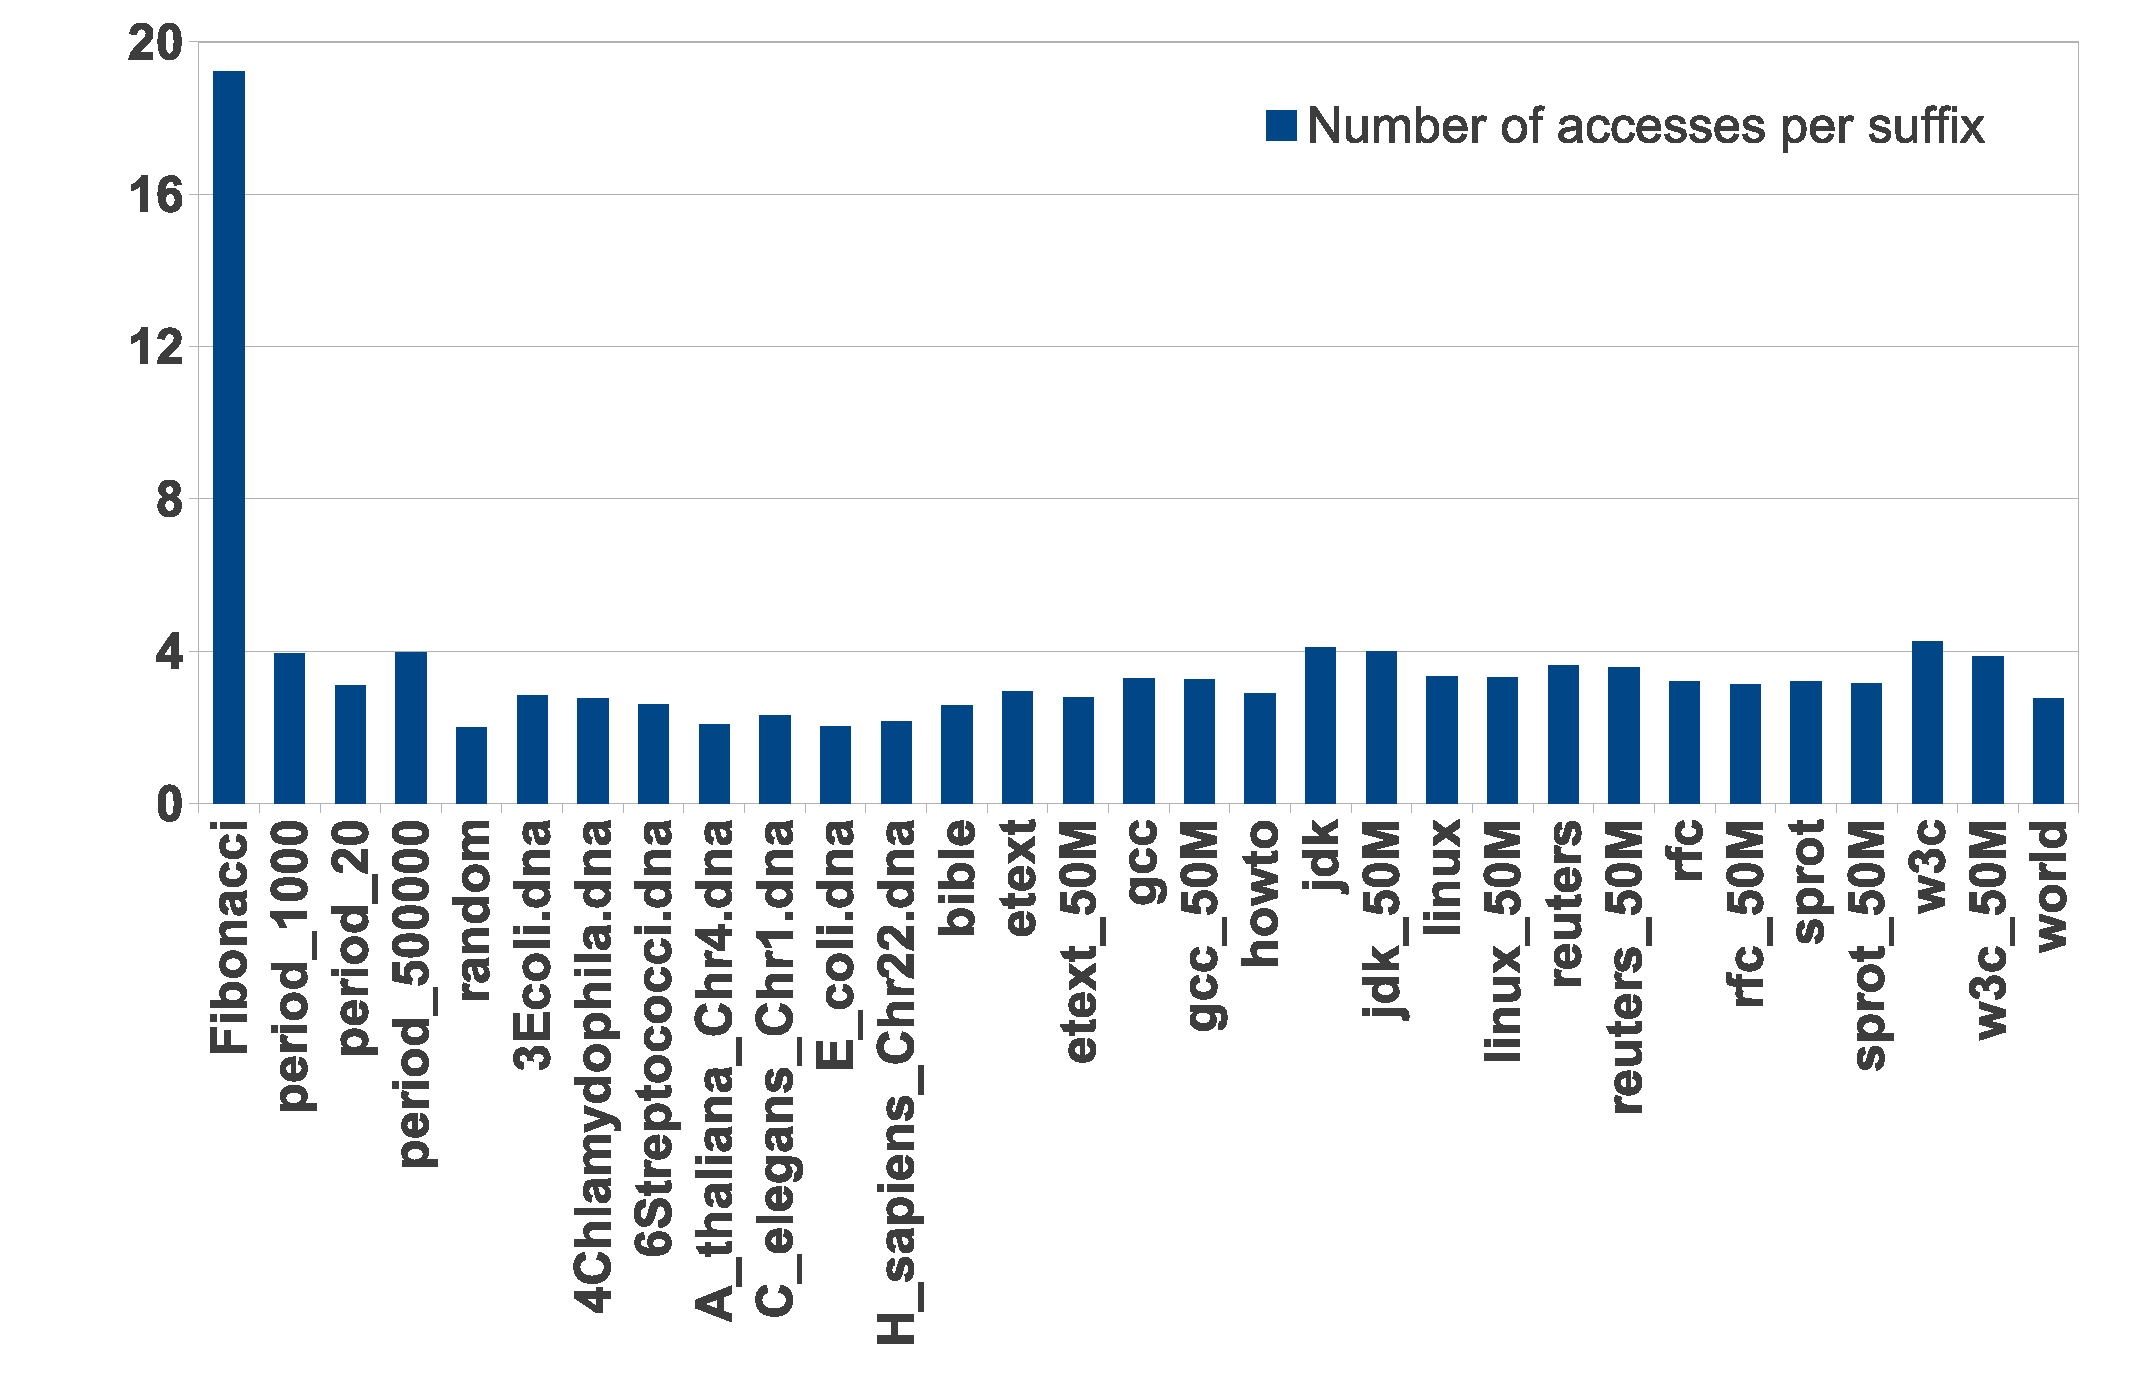
\includegraphics[scale=0.4]{avgAccessPerSuffix.eps}
\end{figure}


\begin{table}
    
    \caption{\label{table_results}Comparison of suffix array construction
    algorithms run times.
    }
    \scalebox{0.75}{
\begin{tabular}{| c | c | c | c | c | c | c |
c | c | c | c |}
\hline 
\multicolumn{3}{| c |}{Dataset} & \multicolumn{8}{ c |}{Run time}  \\
\hline
 &  & & & & & DivSuf &
QSuf & &  & Deep \\
Name & Length & $|\Sigma|$ & RadixSA  & BPR2  & BPR.9 &  Sort &
Sort & SAIS & skew & Shallow 
\\
\hline
Fibonacci & 20000000 & 2 & 7.88 & 12.48 & 14.05 & { 6.81} & 26.44 & {\bf
5.50} & 14.53 & 369.48
\\
\hline
period\_1000 & 20000000 & 26 & {\bf 2.12} & 3.52 & 5.71 &  { 3.15} & 20.42 &
6.59 & 23.27 & TL
\\
\hline
period\_20 & 20000000 & 17 & {\bf 1.44} & 1.95 & 43.39 & { 1.83} & 11.05 &
2.83 & 7.15 & TL
\\
\hline
period\_500000 & 20000000 & 26 & {\bf 2.78} & { 4.60} & 6.31 & 4.74 & 23.32 &
8.56 & 25.68 & 2844.37
\\
\hline
random & 20000000 & 26 & {\bf 2.25} & { 3.34} & 4.87 & 6.35 & 5.02 & 11.75 &
22.05 & 5.69
\\
\hline
3Ecoli.dna & 14776363 & 5 & {\bf 2.23} & { 2.67} & 3.43 & 4.00 & 13.85 & 6.14
& 19.62 & 433.54
\\
\hline
4Chlamydophila.dna & 4856123 & 6 & {\bf 0.61} & { 0.67} & 0.90 & 1.71 & 3.24
& 1.93 & 5.24 & 4.80
\\
\hline
6Streptococci.dna & 11635882 & 5 & {\bf 1.63} & { 1.79} & 2.38 & 2.88 & 7.08
& 4.98 & 14.88 & 4.26
\\
\hline
A\_thaliana\_Chr4.dna & 12061490 & 7 & {\bf 1.27} & { 1.74} & 2.40 & 3.02 &
5.13 & 5.37 & 15.71 & 3.52
\\
\hline
C\_elegans\_Chr1.dna & 14188020 & 5 & {\bf 1.61} & { 1.95} & 2.65 & 3.21 &
6.91 & 5.69 & 17.18 & 6.92
\\
\hline
E\_coli.dna & 4638690 & 4 & {\bf 0.41} & { 0.51} & 0.58 & 1.36 & 1.72 & 1.96
& 5.04 & 1.37
\\
\hline
H\_sapiens\_Chr22.dna & 34553758 & 5 & {\bf 4.40} & { 5.66} & 8.21 & 7.76 &
15.31 & 15.59 & 49.70 & 10.98
\\
\hline
bible & 4047391 & 63 &  { 0.51} & {\bf 0.48} & 0.80 & 1.24 & 1.38 &
1.56 & 4.64 & 1.08
\\
\hline
etext & 105277339 & 146 & {\bf 19.40} & { 23.09} & 43.46 & 26.56 & 62.63 &
54.70 & ML & 119.96
\\
\hline
etext\_50M & 50000000 & 120 & {\bf 8.13} & { 9.74} & 17.26 & 11.94 &
26.40 & 24.46 & 88.57 & 79.07
\\
\hline
gcc & 86630400 & 150 & {\bf 13.84} & { 15.58} & 24.50 & 15.84 & 46.20 & 33.62
& 135.12 & 80.78
\\
\hline
gcc\_50M & 50000000 & 121 & {\bf 7.21} &  9.56 & 13.26 & { 8.31} & 28.43 &
17.73 & 68.65 & 264.90
\\
\hline
howto & 39422104 & 197 & {\bf 5.96} & { 6.35} & 10.26 & 8.41 & 17.64 & 16.67
& 64.73 & 16.33
\\
\hline
jdk & 69728898 & 113 & {\bf 12.07} & { 12.54} & 26.86 & { 12.74} & 39.92 &
24.66 & 102.76 & 58.22
\\
\hline
jdk\_50M & 50000000 & 110 & {\bf 8.32} & {\bf 8.30} & 17.05 & { 8.91} & 26.30
& 17.58 & 71.31 & 36.98
\\
\hline
linux & 116254720 & 256 & {\bf 19.27} & {\bf 19.34} & 29.67 & { 21.17} &
61.99 & 44.47 & ML & 58.71
\\
\hline
linux\_50M & 50000000 & 256 & {\bf 7.62} & {\bf 7.60} & 10.50 & { 8.84} &
27.54 & 18.18 & 76.10 & 31.92
\\
\hline
reuters & 114711150 & 93 & {\bf 19.76} & { 25.08} & 60.72 & { 25.07} &
74.78 & 49.17 & ML & 87.57
\\
\hline
reuters\_50M & 50000000 & 91 & {\bf 7.84} & { 9.53} & 20.41 & 10.24 & 26.94 &
20.29 & 77.25 & 33.68
\\
\hline
rfc & 116421900 & 120 & {\bf 21.18} & { 22.08} & 42.75 & 22.55 & 66.28 &
47.99 & ML & 42.14
\\
\hline
rfc\_50M & 50000000 & 110 & {\bf 8.23} & { 8.39} & 14.85 & 9.24 & 24.80
& 19.61 & 76.64 & 16.63
\\
\hline
sprot & 109617186 & 66 & {\bf 18.48} & { 22.79} & 47.07 & 25.52 & 69.58 &
50.40 & ML & 48.69
\\
\hline
sprot\_50M & 50000000 & 66 & {\bf 7.57} & { 9.10} & 16.81 & 10.88 & 28.07 &
21.69 & 78.47 & 20.03
\\
\hline
w3c & 104201578 & 256 & {\bf 18.82} & {\bf 18.78} & 35.94 & { 20.01} & 74.09
& 38.29 & ML & 1964.80
\\
\hline
w3c\_50M & 50000000 & 255 & {\bf 7.93} & { 8.33} & 17.67 & 8.73 & 25.95 &
17.26 & 71.42 & 36.59
\\
\hline
world & 2473399 & 94 & { 0.30} & {\bf 0.27} &  0.42 & 0.91 & 0.86 & 0.91
& 2.35 & 0.78
\\
\hline
\end{tabular}
}\\
Comparison of suffix array construction
algorithms run times on datasets from \cite{ScSt07} on a 64-bit Intel CORE
i3 machine with 4GB of RAM, Ubuntu $11.10$ Operating System, Sun Java $1.6.0\_26$ and gcc $4.6.1$. Run times are in seconds, averaged over 10 runs. Bold font indicates the
best time. \commentOut{Ties were established
using T-tests.} ML means out of memory, TL means more than 1 hour.
\end{table}  

\section{Discussion and Conclusions}

In this chapter we have presented an elegant algorithm for the construction of
suffix arrays. This algorithm is one of the simplest algorithms known for
suffix arrays construction and runs in $O(n)$ time on a large fraction of all
possible inputs. It is also nicely parallelizable. We have shown how our
algorithm can be implemented on various parallel models of computing. 

We have also given an extension of this algorithm, called RadixSA, which has a worst
case runtime of $O(n \log n)$ and proved to be efficient in practice. 
RadixSA uses a heuristic to select the order in which buckets are 
processed so as to reduce the number of operations performed. RadixSA performed a linear number 
of operations on all but one 
of the inputs tested. The heuristic could find application as an independent speedup technique 
for other algorithms which use bucket sorting and induced copying. For example, BPR could
use it to determine the order in which it chooses buckets to be refined.
A possible research direction is to improve RadixSA's heuristic. Buckets can be processed based on 
a topological sorting of their dependency graph. Such a graph has at most $n/2$ 
nodes, one for each non singleton bucket, and at most $n/2$ edges. Thus, it
has the potential for a lightweight implementation. 
 
An interesting open problem is to devise a randomized algorithm that has a
similar performance. 

\chapter{Pattern Matching With Mismatches}
\section{Introduction}

The problem of string matching has been studied extensively
due to its wide range of applications from Internet searches to computational biology. 
String matching can be defined as follows. Given a text $T=t_1 t_2\cdots
t_n$ and a pattern $P=p_1p_2\cdots p_m$, with letters from an alphabet $\Sigma$,
find all the occurrences of the pattern in the text.
This problem can be solved in $O(n+m)$ time by using well known algorithms
(e.g., KMP \cite{KMP77}). A variation of this problem is to search for
multiple patterns at the same time. An algorithm for this version is given in 
\cite{AC75}. The problem has been generalized to use trees instead of sequences
or to use sets of characters instead of single characters (see \cite{CH99}). 


A more general formulation allows ``don't care'' or ``wild card''
characters in the text and the pattern. A wild card matches any character. An 
algorithm for pattern matching with wild cards is given in \cite{FP74} and has a
runtime of $O(n \log |\Sigma| \log m)$.  The algorithm maps each character in
$\Sigma$ to a binary code of length $\log |\Sigma|$. Then, a constant number of
convolution operations are used to check for mismatches between the
pattern and any position in the text. For the same problem, a randomized algorithm
that runs in $O(n \log n)$ time with high probability is given
in \cite{IND98}. A slightly faster randomized $O(n \log m)$ algorithm is given in
\cite{Kal02}. A simple deterministic $O(n \log m)$ time algorithm based on
convolutions is given in \cite{CC07}.

A more challenging formulation of the problem is pattern matching with
mismatches.
This formulation appears in two versions: a) for every alignment of the
pattern in the text, find the distance between the pattern and the text,
or b) identify only those alignments where the distance between the pattern and the text is less than a given
threshold. The distance metric can be the Hamming distance, edit
distance, $L_1$ metric, and so on. 
A survey of string matching with mismatches is given in \cite{Nav01}.
A description of practical on-line string searching algorithms can be
found in \cite{NR02}.

The algorithms in this chapter are using
the Hamming distance. The Hamming distance between two strings $A$ and $B$, of equal
length, is defined as the number of positions where the two strings differ and is denoted
by $Hd(A,B)$. We are interested in the following two problems, with and without
wild cards.
 

{\bf 1. Pattern matching with mismatches:} Given a text $T=t_1t_2\ldots
t_n$, and a pattern $P=p_1p_2\ldots p_m$, output $Hd(P, t_i t_{i+1}\ldots
t_{i+m-1})$, for every $i,~1\leq i\leq n-m+1$.

{\bf 2. Pattern matching with $k$ mismatches (or the $k$-mismatches problem):}
Take the same input as above, plus an integer $k$. Output all $i$, $1\leq i\leq
n-m+1$, for which $Hd(P, t_i t_{i+1},\ldots t_{i+m-1}) \leq k$.


\subsection{Pattern Matching with Mismatches}

For pattern matching with mismatches, a naive algorithm
computes the Hamming distance for every alignment of the pattern in the
text, in time $O(nm)$. A faster algorithm, in the absence of wild cards, is
Abrahamson's algorithm \cite{ABR87} that runs in $O(n \sqrt{m \log m})$
time.
Abrahamson's algorithm can be extended to solve pattern matching
with mismatches {\em and} wild cards, as we prove in section \ref{sec_glogm}.
The new algorithm runs in $O(n \sqrt{g \log m})$ time, where $g$ is the number of non-wild card positions in the pattern. This gives a simpler and
faster alternative to an algorithm proposed in \cite{ALP04}.

In the literature, we also find algorithms that approximate the number of
mismatches for every alignment. For example, an approximate algorithm for
pattern matching with mismatches, in the absence of wild cards, that runs in $O(r n \log
m)$ time, where $r$ is the number of iterations of the algorithm, is
given in \cite{ACD01}. Every distance reported has a variance bounded by
$(m-c_i)/{r^2}$ where $c_i$ is the exact number of matches for alignment $i$.

Furthermore, a randomized algorithm that approximates the Hamming distance
for every alignment within an $\epsilon$ factor and runs in $O(n
\log^cm/\epsilon^2)$ time, in the absence of wild cards, is given in \cite{KAR93}.
Here $c$ is a small constant. We extend this algorithm to
pattern matching with mismatches {\em and} wild cards, in
section \ref{sec_approx_count_rand}.
The new algorithm
approximates the Hamming distance for every alignment within an $\epsilon$ factor in time
$O(n\log^2m/\epsilon^2)$ with high probability.

Recent work has also addressed the online
version of pattern matching, where the text is received in a
streaming model, one character at a time, and it cannot be stored in its
entirety (see e.g., \cite{CKP08}, \cite{PP09}, \cite{PL07}).
Another version of this problem matches the pattern against multiple input
streams (see e.g., \cite{CEP+07}). Another interesting problem is to sample a
representative set of mismatches for every alignment (see e.g., \cite{CEP+12}).

\subsection{Pattern Matching with $k$ Mismatches}

For the $k$-mismatches problem, without wild cards, two algorithms that
run in $O(nk)$ time are presented in \cite{LV85} and \cite{GG86}. A faster
algorithm, that runs in $O(n\sqrt{k \log k})$ time, is given in
\cite{ALP04}. This algorithm combines the two
main techniques known in the literature for pattern matching with mismatches: filtering and convolutions. 
We give a significantly simpler algorithm in section \ref{sec_nsqrtk}, having
the same worst case run time. The new algorithm will never perform more
operations than the one in \cite{ALP04} during marking and convolution. 
 
An intermediate problem is to check if the
Hamming distance is less or equal to $k$ for a subset of the aligned positions.
This problem can be solved with the Kangaroo method proposed in \cite{GG86} at a
cost of $O(k)$ time per alignment, using $O(n+m)$ additional memory. We show how to achieve the same
run time per alignment using only $O(m)$ additional memory, in section
\ref{sec_k_mism_det}.

Further, we look at the version of $k$-mismatches where wild cards are allowed
in the text and the pattern. For this problem, two randomized algorithms are
presented in \cite{CEP+07}. The first one runs in $O(nk\log n\log m)$  time and
the second one in $O\left (n\log m(k+\log n\log\log n)\right )$ time.
Both are Monte Carlo algorithms, i.e., they output the correct
answer with high probability. The same paper also gives a deterministic
algorithm with a run time of $O(nk^2\log^3m)$. Also, a deterministic $O(nk
\log^2 m(\log^2 k + \log \log m))$ time algorithm is given in \cite{CEPR09}. We present a
Las Vegas algorithm (that always outputs the correct answer), in section
\ref{sec_las_vegas}, which runs in time $O(nk\log^2 m+n\log^2m\log n+n\log
m\log n\log\log n)$ with high probability. Deterministically, pattern matching
with $k$ mismatches and wild cards can be solved in time $O(nk^2\log^2m)$ as shown in
\cite{Clif10}.

If we allow for wild cards in the pattern but not the text, an 
$O(nm^{1/3}k^{1/3}log^{2/3}m)$ time algorithm is given in \cite{CP10}.
We improve this runtime as follows.  Given a pattern $P$, with wild cards, a
maximal length substring of $P$ that has no wild cards is called an ``island''.
We denote the number of islands in $P$ as $q$. In chapter 
\ref{sec_nsqrtk_wild} we give two algorithms for pattern matching with $k$
mismatches where there are wild cards in the pattern.
The first one runs in $O(n\sqrt{(q+k)\log m})$ time. 
The second one runs in time $O(n\sqrt[3]{qk\log^2 m} +
n\sqrt{k\log m})$ where $q$ is the number of islands in $P$. By combining the
two, we show that pattern matching with $k$ mismatches and wild cards in the
pattern can be solved in $O(n\sqrt{k\log m}+n\min\{\sqrt[3]{qk\log^2 m},\sqrt{q\log m}\})$ time.
If the number of islands is $O(k)$ our runtime becomes $O(n\sqrt{k \log m})$,
which essentially matches the best known runtime for pattern matching with $k$
mismatches without wild cards ($O(n\sqrt{k\log k})$). 
 If $q=o(m)$, our algorithm outperforms the
$O(n\sqrt[3]{mk\log^2m})$ run time of \cite{CP07}.  
Therefore, our algorithm is a step
towards bridging the gap between the versions with and without wild cards
cares for pattern matching with $k$ mismatches. 
%ADD
In other words, with the
previous algorithm, even with a few wild cards in the pattern, the
runtime could be much larger than the runtime if there were no wild cards.
In the new algorithm, if the number of wild cards is relatively small
then the runtime is the same as in the version without wild cards.
%%% 



\subsection{Our Results}

The contributions of this chapter can be summarized as follows.

{\bf For pattern matching with mismatches:}
\begin{itemize}
\item An algorithm  for pattern matching with mismatches
and wild cards that runs in $O(n \sqrt{g \log m})$ time, where $g$ is the
number of non-wild card positions in the pattern. See section \ref{sec_glogm}.

\item A randomized algorithm that approximates the Hamming distance for every
alignment, when wild cards are present, within an $\epsilon$ factor in time
$O(n\log^2m/\epsilon^2)$ with high probability. See section
\ref{sec_approx_count_rand}.
\end{itemize}

{\bf For pattern matching with $k$ mismatches:}
\begin{itemize}
\item An algorithm that tests if the Hamming distance is less than $k$
for a subset of the alignments, without wild cards, at a cost of $O(k)$ time per
alignment, using only $O(m)$ additional memory. This achieves the same
runtime per alignment as the Kangaroo method, but with less memory. See section
\ref{sec_k_mism_det}.

\item An algorithm for pattern matching
with $k$ mismatches, without wild cards, that runs in $O(n\sqrt{k \log k})$
time. This algorithm is simpler and has a better expected run time than the one
in \cite{ALP04}. See section \ref{sec_nsqrtk}.

\item An algorithm for pattern matching
with $k$ mismatches with wild cards in the pattern, that runs
in $O(n\sqrt{k\log m}+n\min\{\sqrt[3]{qk\log^2 m},\sqrt{q\log m}\})$ time,
where $q$ is the number of non-wild card islands in the pattern.  If $q=o(m)$,
our algorithm outperforms the $O(n\sqrt[3]{mk\log^2m})$ run time of \cite{CP07}.
See section \ref{sec_nsqrtk_wild}.


\item A Las Vegas algorithm for the
$k$-mismatches problem with wild cards that runs in
time $O(nk\log^2 m+n\log^2m\log n+n\log m\log n\log\log n)$ with high
probability. See section \ref{sec_las_vegas}.
\end{itemize}

These algorithms are also included in our papers \cite{NRKM15} and
\cite{NRKM16}.
The rest of the chapter is organized as follows. First we introduce some notations
and definitions. 
Then we describe the exact, deterministic algorithms for pattern matching with
mismatches and for $k$-mismatches. Then we present the randomized and
approximate algorithms: first the algorithm for approximate counting of
mismatches in the presence of wild cards, then the Las Vegas algorithm for
$k$-mismatches with wild cards. Finally, we present an empirical run time
comparison of the deterministic algorithms, and conclusions.

\section{Materials and Methods}

In terms of notation, $T_{i..j}$ is the substring of $T$ between $i$ and $j$
and $T_i$ stands for $T_{i..i+m-1}$. Furthermore, the value at
position $i$ in array $X$ is denoted by $X[i]$. 

%%%%%%%%%%%%%%%%%%

\subsection{Background}
In this section we review a number of well known
techniques used in the literature for pattern pattern matching with $k$ mismatches (e.g., see
\cite{ALP04}), namely: convolution, marking, filtering and the Kangaroo method.




 

\subsubsection{Convolution}
Given two arrays $T=t_1t_2\ldots t_n$ and $P=p_1p_2\ldots
p_m$ (with $m\leq n$), the convolution of $T$ and $P$ is a sequence
$C=c_1,c_2,\ldots,c_{n-m+1}$ where $c_i=\sum_{j=1}^mt_{i+j-1}p_j$, for $1\leq
i\leq (n-m+1)$. 

The convolution can be applied to pattern matching with mismatches, as follows.
Given a string $S$ and a character $\alpha$ define string $S^{\alpha}$
as $S^\alpha[i]=1$ if $S[i]=\alpha$ and $0$ otherwise.
Let $C^\alpha=convolution(T^\alpha, P^\alpha)$. Then $C^\alpha[i]$ gives the
number of matches between $P$ and $T_i$
where the matching character is $\alpha$. Therefore, one convolution gives us
the number of matches contributed by a single character to each of the
alignments. Then $\sum_{\alpha \in \Sigma}C^{\alpha}[i]$ is the total number of
matches between $P$ and $T_i$.

One convolution can be computed in
$O(n\log m)$ time by using the Fast Fourier Transform. 
If the convolutions are applied on binary inputs, as is often the case in
pattern matching applications, some speedup techniques are presented in \cite{FG09}.

\subsubsection{Marking}\label{sec_marking} 

Marking is an algorithm that counts the number of matches of
every alignment.
Specifically, the algorithm scans the text one character at a time
and ``marks'' all the alignments that would produce a match between the current
character in the text and the corresponding character in the pattern. 

The marking algorithm is generally used only on a subset of the pattern. That
is, given a set $A$ of positions in $P$ the marking algorithm counts matches
between the text and the subset of $P$ given by $A$. The pseudocode of the
marking algorithm is given in Algorithm \ref{alg_counting}.

\begin{algorithm}
\SetKwInOut{Input}{input}\SetKwInOut{Output}{output}
\caption{Mark$(T, P, A)$}\label{alg_counting} 
\Input{Text $T$, pattern $P$ and a set $A$ of positions in $P$} 
\Output{An array $M$ where $M[i]$ gives the number of matches between $T_i$
and $P$, on the subset of positions of $P$ given by $A$}
\lFor {$i\leftarrow 1$ \KwTo $n$}{$M[i]=0$}
\For {$i\leftarrow 1$ \KwTo $n$}{
  \For{$j \in A$ s.t. $P[j] = T[i]$}{
    \lIf{$i-j+1 > 0$}{
      $M[i-j+1]${\bf $++$}
    }
  }
}
\Return $M$\;
\end{algorithm}

\subsubsection{Filtering}
The marking algorithm in the previous section is generally followed by a
filtering method. Filtering is based on the following principle. If we restrict
our pattern to only $2k$ positions, any alignment that has no more than
$k$ mismatches, must have at least $k$ matches among the $2k$ positions.
To count matches among the $2k$ positions selected, for every alignment, we use
the marking algorithm. If the total number of marks generated is $B$ then there
can be no more than $B/k$ positions that have at least $k$ marks (i.e.,
matches). The alignments that have at least
$k$ marks are further inspected using the Kangaroo method.

\subsubsection{The Kangaroo method}\label{sec_kangaroo} 

The Kangaroo method allows us to check if the number of mismatches for a
particular alignment is no more than $k$, in $O(k)$ time. The Kangaroo method
constructs a generalized suffix tree of $T\#P$ where $\#$ means concatenation.
This suffix tree can be enhanced to answer Lowest Common Ancestor
(LCA) queries in $O(1)$ time \cite{AH+76}. LCA queries give us the longest
common prefix between any portion of the text and any portion of the pattern,
essentially telling us where the first mismatch appears. 
Specifically, to count mismatches between
$P$ and $T_i$, first perform an LCA query to find the position of the
first mismatch between $P$ and $T_i$. Let this position be $j$. Then,
perform another LCA to find the first mismatch between $P_{j+1..m}$ and
$T_{i+j+1.. i+m-1}$, which gives the second mismatch of alignment $i$.
Continue to ``jump'' from one mismatch to the next, until the end
of the pattern is reached or we have found more than $k$ mismatches.
Therefore, after $O(k)$ LCA queries we will either find all the mismatches or
determine that there are more than $k$ of them. 
The Kangaroo pseudocode is given in Algorithm \ref{alg_kangaroo}.

\begin{algorithm}
\SetKw{LCA}{LCA}
\SetKw{True}{true}
\SetKw{False}{false}
\SetKwInOut{Input}{input}\SetKwInOut{Output}{output}
\caption{Kangaroo$(P, T_i, k)$}\label{alg_kangaroo}
\Input{A pattern $P$, an alignment $T_i$ and an integer $k$}
\Output{\True if the pattern matches the alignment with no more than $k$
mismatches, \False otherwise}
$j=0$\;
$d=0$\;
\While{$d \leq k$} {
  $j = j + \LCA(T_{i+j}, P_j)+1$\;
  \If {$j > m$} {
     \Return{\True}\;
  }
  $d=d+1;$
}  
\Return{\False}\;
\end{algorithm}

\subsubsection{Probability Bounds}
 
In the context of randomized algorithms, by
high probability we mean a probability greater or equal to $(1-n^{-\epsilon})$ 
where $n$ is the input size and $\epsilon$ is a probability parameter usually
assumed to be a constant greater than $0$. The run time of a Las Vegas algorithm
is said to be $\widetilde O(f(n))$ if the run time is no more than $c\epsilon f(n)$
with probability greater or equal to $(1-n^{-\epsilon})$ for all $n\geq n_0$,
where $c$ and $n_0$ are some constants, and for any constant $\epsilon\geq 1$.


In the analysis of our algorithms, we will employ the following Chernoff bounds.


\noindent{\bf Chernoff Bounds} \cite{Che52}.
These bounds can be used to closely
approximate the tail ends of a binomial distribution.

A Bernoulli trial has two outcomes namely {\em success} and {\em failure},
the probability of success being $p$. A binomial distribution with
parameters $n$ and $p$, denoted as $B(n,p)$, is the number of successes
in $n$ independent Bernoulli trials.

Let $X$ be a binomial random variable whose distribution is
$B(n,p)$. If $m$ is any integer $>np$, then the following are true:
\begin{equation}\label{eq_chernoff1}
Prob.[X>m]~\leq~\left (\frac{np}{m}\right )^m~e^{m-np};
\end{equation}

\begin{equation}\label{eq_chernoff2}
Prob.[X>(1+\delta)np]~\leq~e^{-\delta^2np/3};~{\rm and}
\end{equation}

\begin{equation}\label{eq_chernoff3}
Prob.[X<(1-\delta)np]~\leq~e^{-\delta^2np/2}
\end{equation}
 for any
$0<\delta<1$.

\subsection{Exact Algorithms for Pattern Matching with Mismatches}


For pattern matching with mismatches, without wild cards,
the following $O(n\sqrt{m \log m})$ time algorithm was given by Abrahamson
\cite{ABR87}.
Let $A$ be a set of the most frequent characters
in the pattern. 1) Using convolutions, count how many matches each character in $A$ contributes to
every alignment. 2) Using marking, count how many matches each character
in $\Sigma - A$ contributes to every alignment. 3) Add the two
numbers to find for every alignment, the number of matches between the pattern
and the text. The convolutions take $O(|A| n \log m)$ time. A
character in $\Sigma - A$ cannot appear more than $m/|A|$ times in the pattern,
otherwise, each character in $A$ has a frequency greater than
$m/|A|$, which is not possible. Thus, the run time for marking is $O(n m / |A|)$.
If we equate the two run times we find the optimal $|A| = \sqrt{m / \log m}$ which gives a
total run time of $O(n \sqrt{m \log m})$.


\noindent{\bf An Example.} Consider the case of $T=2~3~1~1~4~1~2~3~4~4~2~1~1~3~2$ and $P=1~2~3~4$. Since each character in the pattern occurs an equal number of times, we can pick $A$ arbitrarily. Let $A=\{1,2\}$. In step 1, convolution is used to count the number of matches contributed by each character in $A$. We obtain an array $M_1[1:12]$ such that $M_1[i]$ is the number of matches contributed by characters in $A$ to the alignment of $P$ with $T_i$, for $1\leq i\leq 12$. In this example, $M_1=[0,0,1,1,0,2,0,0,0,1,0,1]$. In step 2 we compute, using marking, the number of matches contributed by the characters $3$ and $4$ to each alignment between $T$ and $P$. We get another array $M_2[1:12]$ such that $M_2[i]$ is the number of matches contributed by $3$ and $4$ to the alignment between $T_i$ and $P$, for $1\leq i\leq 12$. Specific to this example, $M_2=[0,1,0,0,0,2,1,0,0,0,0,1]$. In step 3, we add $M_1$ and $M_2$ to get the number of matches between $T_i$ and $P$, for $1\leq i\leq 12$. In this example, this sum yields: $[0,1,1,1,0,4,1,0,0,1,0,2]$.


\subsubsection{Pattern matching with mismatches and wild cards in $O(n\sqrt{g
\log{g}})$}
\label{sec_glogm}
For pattern matching with mismatches and wild cards, 
a fairly complex algorithm is given in \cite{ALP04}. The run time of this
algorithm is $O(n \sqrt{g} \log m)$ where $g$ is the number of non-wild card
positions in the pattern. The problem can also be solved through a simple modification of 
Abrahamson's algorithm, in time $O(n\sqrt{m \log m})$, as pointed out in 
\cite{CEP+07}. We now prove the following result:

\begin{theorem}
\label{thm_glogm}
 Pattern matching with mismatches and wild cards can be solved
in $O(n\sqrt{g \log m})$ time, where $g$ is the number of non-wild card
positions in the pattern.
\end{theorem}

\begin{proof}
 Ignoring the wild cards for now, let $A$ be the set of
the most frequent characters in the pattern. As above, count matches contributed
by characters in $A$ and $\Sigma-A$ using convolution and marking, respectively.
By a similar reasoning as above, the characters used in the marking phase will not 
appear more than $g / |A|$ times in the pattern. If we equate the run times for the two 
phases we obtain $O(n \sqrt {g \log m})$ time. We are now left to count how many matches are
contributed by the wild cards. For a string $S$ and a character $\alpha$, define $S^{\neg \alpha}$ as
$S^{\neg \alpha}[i] = 1-S^\alpha[i]$. Let
$w$ be the wild card character. Compute $C = convolution(T^{\neg w}, P^{\neg w})$. Then,
for every alignment $i$, the number of positions that have a wild card either in the
text or the pattern or both, is $m-C[i]$. Add $m-C[i]$ to the previously computed counts and output. 
The total run time is $O(n \sqrt{g \log m})$.
\end{proof}

\subsection{Exact Algorithms for Pattern Matching with $k$ Mismatches}
\label{sec_k_mism_det}

For the $k$-mismatches problem, without wild cards, an $O(k(m\log m+n))$ time
algorithm that requires $O(k(m+n))$ additional space is presented in \cite{LV85}. Another algorithm, that takes
  $O(m\log m + kn)$ time and uses only $O(m)$ additional space is presented
in \cite{GG86}. \commentOut{In the latter, a suffix tree of the pattern is built and enhanced to
support lowest common ancestor queries in $O(1)$ time.} We define the following
problem which is of interest in the discussion.

\subsubsection{The Subset $k$-mismatches problem}
\begin{problem}
{\bf Subset $k$-mismatches:} Given a text $T$ of length $n$, a pattern $P$ of
length $m$, a set of positions $S=\{i|1 \leq i \leq n-m+1\}$ and an integer $k$, output the
positions $i \in S$ for which $Hd(P, T_i) \leq k$.
\end{problem}

The Subset $k$-mismatches problem becomes the regular $k$-mismatches
problem if $|S|=n-m+1$. Thus, it can be solved by the $O(nk)$ algorithms mentioned
above. However, if $|S| << n$ then the
$O(nk)$ algorithms are too costly.
A better alternative is to use the Kangaroo method proposed in \cite{ALP04} and
described in section \ref{sec_kangaroo}. The Kangaroo method can verify if
$Hd(P, T_i)\leq k$ in $O(k)$ time for any $i$. The
Kangaroo method can process $|S|$ positions in $O(n+m+|S|k)$ time and it
uses $O(n+m)$ additional memory for the LCA enhanced suffix tree.
The memory requirement can be improved as follows:

\begin{theorem}
{\bf Subset $k$-mismatches} can be solved in $O(n+m+|S|k)$ time using only
$O(m)$ additional memory.
\end{theorem}


\begin{proof}
The algorithm  is the following. Build an LCA-enhanced suffix tree
 of the pattern. Scan the text from left to right. 1) Find the longest unscanned region
of the text that can be found somewhere in the pattern, say starting at
position $i$ of the pattern. Call this region of the text $R$. Therefore, $R$ is
identical to $P_{i..i+|R|-1}$. 2) For every alignment in $S$ that overlaps $R$, count
the number of mismatches between $R$ and the alignment, within the overlap
region.
To do this, consider an alignment in $S$ which overlaps $R$ such that the
beginning of $R$ aligns with the $j$-th character in the pattern. We want to count the number of mismatches between R and $P_{j..j+|R|-1}$. However, since $R$ is identical to
$P_{i..i+|R|-1}$, we can simply compare $P_{i..i+|R|-1}$ and
$P_{j..j+|R|-1}$. This comparison can be done efficiently by jumping from one
mismatch to the next, like in the Kangaroo method. Repeat from step 1 until the
entire text has been scanned.
Every time we process an alignment, in step 2, we either discover at least one additional
mismatch or we reach the end of the alignment.
This is true because, otherwise, the alignment
would match the text for more than $|R|$ characters, which is not possible, from
the way we defined $R$. Every alignment for which we have found more than $k$
mismatches is excluded from further consideration to ensure
$O(k)$ time per alignment. It takes $O(m)$ time to build the LCA enhanced suffix tree of the pattern and
$O(n)$ additional time to scan the text from left to right. Thus, the total run time is
$O(n+m+|S|k)$ with $O(m)$ additional memory. The pseudocode is given in
Algorithm \ref{alg_subsetk}.
\end{proof}

{\LinesNumberedHidden
\begin{algorithm}
\SetKw{And}{and}
\SetKwFunction{updateMism}{countMismatches}
\SetKwFunction{lcp}{lcp}
\SetKwInOut{Input}{input}\SetKwInOut{Output}{output}
\caption{Subset $k$-mismatches($S, T, P, k$)}\label{alg_subsetk} 
\Input{$S$ - set of positions in the text; $T_{1..n}$ - text; $P_{1..m}$
-pattern; k - max number of mismatches\;} 
\Output{$M$ - the positions in $S$ for which the pattern matches the text with
at most $k$ mismatches\;} 
\Begin{
Assume we have a suffix tree/array of the pattern\;
\lFor {$a \in S$}{$M[a]=0$}
$i=1$ \;
\While{$i \leq n$} {
Find the largest $l$ such that $T_{i..i+l-1}$ describes a path in the suffix
tree\; 
This means that $T_{i..i+l-1} = P_{j..j+l-1}$ for some $j$\;
\For{$a \in S$ {\bf where} $a \leq i < a + m$} { 
$M[a] =$ \updateMism$(M[a],
i-a+1, j, l)$ \;
\lIf{$t_{i+l}\neq p_{j+l}$}{$M[a]=M[a]+1$}
\lIf {$M[a] > k$} {$S = S - \{a\}$}
}
$i = i + l + 1$ \;
}
\Return{$\{a \in S | M[a]\leq k\}$}
}
\SetKwProg{myproc}{function}{}{}
\myproc{\updateMism{$c, s_1, s_2, l$}}{
\Input{$c$ - current number of mismatches; $s_1, s_2$ - starting positions of
two suffixes of the pattern; $l$ - a maximum length\;}
\Output{compare the two suffixes on their first $l$ positions and add to $c$
the number of mismatches found; if $c$ exceeds $k$, return $k+1$,
otherwise return the updated $c$ \;} 
\Begin{ \While{$l > 0$  \And $c \leq k$}{
  $d = \lcp(s_1,s_2)$; // longest common prefix\\
  \lIf {$d \geq l$}{\Return {$c$}} 
  $c = c + 1$\;
  $d = d + 1$\;
  $s_1 = s_1 + d$\;
  $s_2 = s_2 + d$\; 
  $l = l - d$\;
}
}
\Return{$c$}
}
\end{algorithm}
}


\subsubsection{An $O(n\sqrt{k \log k})$ Time Algorithm for $k$-Mismatches
without Wild Cards}
\label{sec_nsqrtk}
 
For the $k$-mismatches problem, without wild cards, a fairly complex 
$O(n \sqrt{k \log k})$ time algorithm  is given in \cite{ALP04}. 
The algorithm classifies the inputs into several cases. For each case
it applies a combination of marking followed by a filtering step, the Kangaroo
 method, or convolutions. The goal is to not exceed $O(n \sqrt{k \log k})$ time 
 in any of the cases.
We now present an algorithm with only two cases which has the same worst case run time.
The new algorithm can be thought of as a generalization of the algorithm in \cite{ALP04} 
as we will discuss later.
This generalization not only greatly simplifies the algorithm but it also
reduces the expected run time. This happens because we use information about the frequency of the
characters in the text and try to minimize the work done by convolutions and marking.

We will now give the intuition for this algorithm. For any
character $\alpha \in \Sigma$, let $f_\alpha$ be its frequency in the pattern,
and $F_\alpha$ be its frequency in the text. Note that in the marking algorithm,
a specific character $\alpha$ will contribute to the runtime a cost of
$F_{\alpha} \times f_{\alpha}$. On the other hand, in the case of convolution, a
character $\alpha$ costs us one convolution, regardless of how frequent $\alpha$
is in the text or the pattern. Therefore, we want to use infrequent
characters for marking and frequent characters for convolution. The balancing of
the two will give us the desired runtime.

A position $j$ in
the pattern where $p_j = \alpha$ is called an {\em instance} of $\alpha$. 
Consider every instance of character $\alpha$ as an object of size
$1$ and cost $F_\alpha$. We want to fill a knapsack of size $2k$ at a minimum
cost and without exceeding a given budget $B$. The $2k$
instances will allow us to filter some of the alignments with more
than $k$ mismatches, as it will become clear later. This
problem can be optimally solved by a greedy approach where we include in the knapsack all the instances of the least expensive character, then all the instances of the second least expensive character and so on, until we have $2k$ items or we have exceeded $B$. The last
character considered may have only a subset of its instances included, but for
ease of explanation assume that there are no such characters.

{\bf Note:} Even though the above is described as a Knapsack problem, the
particular formulation can be optimally solved in linear time. This formulation should not be
confused with other formulations of the Knapsack problem that are NP-Complete.

Case 1) Assume we can fill the knapsack at a cost $C \leq B$. We apply the
marking algorithm for the characters whose instances are included in the
knapsack. It is easy to see that the marking takes time $O(C)$ and creates $C$
marks. For alignment $i$, if the pattern and the text match for all the $2k$
positions in the knapsack, we will obtain exactly $2k$ marks at position $i$. 
Conversely, any position which has less than $k$ marks must have more
than $k$ mismatches, so we can filter it out. Therefore, there will be at
most $C/k$ positions with $k$ marks or more. For such positions we run Subset
$k$-mismatches to confirm which of them have less than $k$ mismatches.
The total runtime of the algorithm in this case is $O(C)$.

Case 2) If we cannot fill the knapsack within the given budget $B$ we do the
following: for the characters we could fit in the knapsack, we use the marking
algorithm to count the number of matches they contribute to each alignment. For
characters not in the knapsack, we use convolutions to count the number of
matches they contribute to each alignment. We add the two counts and get the
exact number of matches for every alignment. 

Note that at
least one of the instances in the knapsack has a cost larger than $B/(2k)$ (if
all the instances in the knapsack had a cost less or equal to $B/(2k)$ then we would
have at least $2k$ instances in the knapsack). Also note that all the
instances not in the knapsack have a cost at least as high as any instance in
the knapsack, because we greedily fill the knapsack starting with the least
costly instances. This means that every character not in the knapsack appears
in the text at least $B/(2k)$ times. This means that the number of characters
not in the knapsack does not exceed $n/(B/(2k))$. Therefore the total cost of
convolutions is $O(nk/B\log m)$. Since the cost of marking was $O(B)$ we can see
that the best value of $B$ is the one that equalizes the two costs. This gives
$B=O(n\sqrt{k\log m})$. Therefore, the algorithm takes $O(n\sqrt{k\log m})$
time. If $k < m^{1/3}$  we can employ a different algorithm
that solves the problem in linear time, as in \cite{ALP04}. For larger $k$,
$O(\log m) = O(\log k)$ so the run time becomes $O(n \sqrt{k \log k})$. We call this algorithm
{Knapsack $k$-mismatches}. The pseudocode is given in algorithm
\ref{alg_knapsack}. The following theorem results.


\begin{theorem}
{\bf Knapsack $k$-mismatches} has worst case run time $O(n \sqrt{k \log
k})$.$\square$
\end{theorem}

{\LinesNumberedHidden
\begin{algorithm}
\SetKw{And}{and}
\SetKwFunction{Mark}{Mark}
\SetKwFunction{convolution}{convolution}
\SetKwFunction{subsetk}{Subset $k$-mismatches}
\SetKwInOut{Input}{input}\SetKwInOut{Output}{output}
\caption{Knapsack $k$-mismatches($T, P, k$)}\label{alg_knapsack}
\Input{$T_{1..n}$ - text; $P_{1..m}$ -pattern; k - max number of mismatches\;} 
\Output{$S$ - set of positions in the text where the pattern matches with at
most $k$ mismatches\;} 
\Begin{
Compute $F_i$ and $f_i$ for every $i \in \Sigma$ \;
Sort $\Sigma$ with respect to $F_i$ \;
$s = 0$\;
$c = 0$\;
$i = 1$\;
$B = n \sqrt{k \log k}$ \;
\While{$s < 2k$ \And $c < B$} {
  $t = \min(f_i, 2k - s)$ \;
  $s = s + t$ \;
  $c = c + t \times F_i$ \;
  $i = i + 1$ \;
}
$\Gamma = \Sigma[1..i]$ \;
$M = \Mark(T, n, \Gamma)$; // $M$ counts matches\\
\eIf {$s = 2k$} {
  $S = \{i | M[i] \geq k\}$  \;
  \Return \subsetk($S, T, P, k$)\;
}{
  \For{$\alpha \in \Sigma - \Gamma$} {
    $C = \convolution(T^{\alpha}, P^{\alpha})$ \;
    \For {$i \leftarrow 1$ \KwTo $n$} {
      $M[i] = M[i] + C[i]$ \;
    }
  }
  $S = \{i | M[i] \geq m-k\}$\;    
  \Return{$S$}\;
}
}
\end{algorithm}
}

We can think of the algorithm in \cite{ALP04} as a special case of our
algorithm where, instead of trying to minimize the cost of the $2k$ items in the
knapsack, we just try to find $2k$ items for which the cost is less than
$O(n\sqrt{k \log m})$. As a result, it is easy to verify the following:
\begin{theorem}\label{knapsack_less}
{\bf Knapsack $k$-mismatches} spends at most as much time as
the algorithm in \cite{ALP04} to do convolutions and marking.
\end{theorem}

\begin{proof}
{\bf Observation:} In all the cases presented below,
Knapsack $k$-mismatches can have a run time as low as $O(n)$, for example if
there exists one character $\alpha$ with $f_\alpha = O(k)$ and $F_\alpha = O(n/k)$.

{\bf Case 1:} $|\Sigma| \geq 2k$. The algorithm in \cite{ALP04} chooses $2k$
instances of distinct characters to perform marking. Therefore, for every
position of the text at most one mark is created. If the number of
marks is $M$, then the cost of the marking phase is $O(n + M)$.
The number of remaining positions after filtering is no more than $M/k$ and thus the algorithm takes
$O(n+M)$ time.
Our algorithm puts in the knapsack 2k instances, of not necessarily different
characters, such that the number of marks $B$ is minimized! Therefore $B \leq M$
and the total runtime is $O(n+B)$.

{\bf Case 2:} $|\Sigma| < 2\sqrt{k}$. The algorithm in \cite{ALP04} performs
one convolution per character to count the total number of matches for every
alignment, for a run time of $\Omega(|\Sigma|n\log m)$. In the worst case, 
Knapsack $k$-mismatches cannot fill the knapsack at a cost $B < |\Sigma|n\log
m$ so it defaults to the same run time. However, in the best case, the
knapsack can be filled at a cost $B$ as low as $O(n)$ depending on the
frequency of the characters in the pattern and the text. In this case the
runtime will be $O(n)$.

{\bf Case 3:} $2\sqrt{k} \leq |\Sigma| \leq 2k$. A symbol that appears in the
pattern at least $2\sqrt{k}$ times is called frequent.

{\bf Case 3.1:} There are at least $\sqrt{k}$ frequent symbols. The algorithm in
\cite{ALP04} chooses $2\sqrt{k}$ instances of $\sqrt{k}$ frequent symbols to do
marking and filtering at a cost $M \leq 2n\sqrt{k}$. Since Knapsack
$k$-mismatches will minimize the marking time $B$ we have
$B \leq M$ so the run time is the same as for \cite{ALP04} only in the worst
case.

{\bf Case 3.2:} There are $A < \sqrt{k}$ frequent symbols. The
algorithm in \cite{ALP04} first performs one convolution for each frequent
character for a run time of $O(A n \log m)$.
Two cases remain:

{\bf Case 3.2.1:} All the instances of the non-frequent symbols number less than
$2k$ positions. The algorithm in \cite{ALP04} replaces all instances of frequent
characters with wild cards and applies a $O(n\sqrt{g} \log{m})$ algorithm to
count mismatches, where $g$ is the number of non-wild card positions. Since
$g<2k$ the run time for this stage is $O(n\sqrt{k} \log{m})$ and the total
run time is $O(An\log m + n\sqrt{k} \log{m})$.
Knapsack $k$-mismatches can always include in the knapsack all the
instances of non-frequent symbols since their total cost is no more than
$O(n\sqrt{k})$ and in the worst case do convolutions for the remaining
characters. The total run time is $O(An\log m + n\sqrt{k})$. Of course,
depending on the frequency of the characters in the pattern and text, Knapsack
$k$-mismatch may not have to do any convolutions.

{\bf Case 3.2.2:} All the instances of the non-frequent symbols number at
least $2k$ positions. The algorithm in \cite{ALP04} chooses $2k$ instances of
infrequent characters to do marking. Since each character has frequency less
than $2\sqrt{k}$, the time for marking is $M < 2n\sqrt{k}$ and there are no more
than $M/k$ positions left after filtering. Knapsack
$k$-mismatches chooses characters in order to minimize the time $B$
for marking, so again $B \leq M$.
\end{proof}

\subsection{Algorithms for $k$-Mismatches with Wild Cards in the Pattern}
\label{sec_nsqrtk_wild}

In this section we consider pattern matching with $k$ mismatches
where there could be some wild cards in the pattern.  Given a pattern $P$,
with wild cards, a maximal length substring of $P$ that has no wild cards is called an ``island''.
We will denote the number of islands in $P$ as $q$.

For this problem, an algorithm that
runs in $O(nm^{1/3}k^{1/3}log^{2/3}m)$ time is given in \cite{CP10}.
We improve this runtime as follows.  We give two algorithms for pattern matching
with $k$ mismatches where there are wild cards in the pattern.
The first one runs in $O(n\sqrt{(q+k)\log m})$ time. 
The second one runs in time $O(n\sqrt[3]{qk\log^2 m} +
n\sqrt{k\log m})$ where $q$ is the number of islands in $P$. By combining the
two, we show that pattern matching with $k$ mismatches and wild cards in the
pattern can be solved in $O(n\sqrt{k\log m}+n\min\{\sqrt[3]{qk\log^2 m},\sqrt{q\log m}\})$ time.

If the number of islands is $O(k)$ our runtime becomes $O(n\sqrt{k \log m})$,
which essentially matches the best known runtime for pattern matching with $k$
mismatches without wild cards ($O(n\sqrt{k\log k})$).
 If $q=o(m)$, our algorithm outperforms the $O(n\sqrt[3]{mk\log^2m})$ run time
 of \cite{CP07}. 
 
Both algorithms in this section have the same basic structure. The
difference is in how fast we can verify whether the distance between $P$ and a given alignment
is no more than $k$. In other words, the difference is in how fast we can answer
the single alignment verification question:

\begin{question}
Given i, is the distance between $P$ and $T_i$ no more than $k$?
\end{question}

In the first algorithm, we can answer this question in $O(q+k)$ time. In the
second algorithm, we can answer this question in $O(\sqrt[3]{k^2q^2\log
m} + k)$ time.

The general structure of both the algorithms is given in Algorithm
\ref{alg_basic} and is essentially a slight generalization of the Knapsack
$k$-mismatches algorithm of section \ref{sec_nsqrtk}.


\begin{algorithm}
\caption{$K$-Mismatches with Wild Cards}\label{alg_basic}
Let $F_a$ be the number of occurrences of character $a$ in $T$ for all $a \in
\Sigma$\; 
Let $Cost(A)=\Sigma_{i \in A}F_{P[i]}$\;
Let $A$ be a set of positions in $P$ such that $|A|\leq 2k$
and $Cost(A) \leq B$\; 
$M=Mark(T, P, A)$\;
\eIf{$|A| == 2k$}{
   $R=\{\}$\;
   \For{$i=1$ to $n$} {
      \If {$M_i \geq k$ {\bf and} $DistNoMoreThanK(T_i, P, k)$} {
          $R = R \cup \{i\}$\;
      }
   }
}{
   
   \For{$a \in \Sigma$ s.t. $a \neq P[i], \forall i \in A$} {
      $M'=Convolution(T,P,a)$\;
      $M+=M'$\;
   }
   $R = \{i \in [1..n] | M_i \geq m - k\}$\;  
}
\Return{$R$}\;
\end{algorithm}

{\bf Algorithm and analysis:} 
For each position $i$ in $P$ such that $P[i]=a$, we assign a cost $F_a$ where
$F_a$ is the number of occurrences of $a$ in $T$. The algorithm starts by
choosing up to $2k$ positions from the pattern such that the total cost does not exceed a ``budget''
$B$. The positions are chosen by a simple greedy strategy. Sort all the
characters by their cost $F_a$. Start choosing positions equal to the ``cheapest''
character, then choose positions equal to the next cheapest character, and
so on until we have chosen $2k$ positions or we have exceeded the budget $B$.

{\bf Case 1:} If we can find $2k$ positions that cost no more than $B$, then
we call the marking algorithm with those $2k$ positions. Any
position in $T$ that receives less than $k$ marks, has more than $k$ mismatches,
so we now focus on positions in $T$ that have at least $k$ marks.
If the total number of marks is $B$, then there will be no more than
$B/k$ positions that have at least $k$ marks. We verify each of these
positions to see if they have more than $k$ mismatches. Let the time for a
single verification be $O(V)$.
Then, the runtime is $O(BV/k)$.

{\bf Case 2:} If we cannot find $2k$ positions that cost no more than $B$,
then we compute marking for the positions that we did choose before we ran out
of budget.
Then, for each of the characters that we did not choose, we compute one
convolution to count how many matches they contribute to each alignment. It
is easy to see that each of the characters not chosen for marking must have $F_a
> B/(2k)$.
Therefore, the total number of such characters is no more than $n/(B/(2k))$. Therefore, the runtime of the convolution stage is $O(nk/B * n \log m)$. The runtime of the marking
stage is $O(B)$, therefore the total runtime is $O(B + nk/B * n \log m)$.

If we make the runtime of the two cases equal, we can find the optimal value of
$B$.

\begin{align*}
BV/k = B+n^2k/B \log m \Rightarrow B=nk\sqrt{\frac{\log m}{V}}
\end{align*}

This gives an asymptotic runtime of $O(BV/k)=O(n\sqrt{V \log m})$. Therefore,
the runtime of the algorithm depends on $V$, which is the time it takes to
verify whether a given single alignment has no more than $k$ mismatches.
 
\subsubsection{Single alignment distance in $O(q+k)$ time}
\label{sec_alg1}

We can answer the single alignment question 
in $O(q+k)$ time where $q$ is the number of {\it islands} in the pattern as
shown in Algorithm \ref{alg_verif1}.
The algorithm uses Kangaroo jumps \cite{LV85} to go to the next mismatch within
an island in $O(1)$ time. If there is no mismatch left in the island, the algorithm goes
to the next island also in $O(1)$ time.
Therefore, the runtime is $O(q+k)$. With $V=O(q+k)$, Algorithm \ref{alg_basic} does pattern matching
with $k$ mismatches in $O(n\sqrt{(q+k)\log m})$ time.


\begin{algorithm}
\caption{KangarooDistNoMoreThanK$(T_i, P, k)$}
\label{alg_verif1}
$d=0$\;
$j=0$\;
\While{$d \leq k$ {\bf and} $j < q$}{
  $r =$ no. of mismatches between island $j$ and
  corresponding region of $T_i$ (use Kangaroo jumps)\; 
  $d += r$\; 
  $j += 1$\;   
}
\Return{$d \leq k$}
\end{algorithm}

\subsubsection{Single alignment distance in $O(\sqrt[3]{k^2q^2\log
m}+k)$ time}
\label{sec_alg2}
This idea is based on splitting the pattern into sections. We know that no more
than $k$ sections can have mismatches. The remaining sections have to match
exactly. Consider exact pattern matching with wild cards.
We can check where a pattern matches the text exactly by using a constant number of convolutions. This is
true because we can compute the values $C_i = \Sigma_{j=0}^{m-1}(T_{i+j}-P_j)^2T_{i+j}P_j$ using a constant
number of convolutions (see  \cite{CC07}). If $C_i=0$ then the pattern matches
the text at position $i$. 

Using this result, we will split the pattern into $S$
sections. In each section we include $q/S$ islands. For each of the $S$
sections, we use a constant number of convolutions to check where the section
matches the text. If $P$ has no more than $k$ mismatches at a particular
alignment, then at least $S-k$ sections have to match exactly. Each of the at
most $k$ sections that do not match exactly are verified using Kangaroo jumps as seen
earlier. One section takes at most $O(q/S+k')$ time, where $k'$ is the number
of mismatches discovered in that section. Over all the sections, the $k'$
terms add up to no more than $k$, therefore the entire alignment can be verified
in time $O(S+k+kq/S)$.


If we make $V=O(S + k + kq/S)$ in Algorithm \ref{alg_basic}, then its runtime
becomes $O(n \sqrt{V\log m}) = O(n \sqrt{(S + k + kq/S)\log m})$. 
The preprocessing time for the $S$ sections is $O(Sn \log m)$. The
optimal value of $S$ is such that the preprocessing equals the main runtime:

\begin{align*}
 & n \sqrt{(S + k + kq/S)\log m} = Sn \log m \\
\Rightarrow & S + k + kq/S = S^2 \log m\\
\Rightarrow & S^2/\log m + kS/\log m + kq/\log m = S^3\\
\Rightarrow & S \approx O(\sqrt[3]{kq/\log m})
\end{align*}

This makes $V=O(S + k + kq/S)=
O(k +\sqrt[3]{k^2q^2\log m})$. This gives a
runtime for pattern matching with $k$ mismatches of:

\begin{align*}
O(nS\log m + n \sqrt{V\log m}) = & O\left(n\sqrt[3]{kq\log^2
m} + n\sqrt{ (k + \sqrt[3]{k^2q^2\log m}) \log m   }\right)\\
= & O\left( n \sqrt[3]{kq\log^2 m} +  n\sqrt{k \log m} \right)\\
\end{align*}

\subsubsection{Combined result}
If $q < k^2$ then we can use the algorithm of section
\ref{sec_alg1}, which runs in $O(n\sqrt{(q+k)\log m})$ time. Otherwise, if
$q > k^2$, we use the algorithm of section \ref{sec_alg2}, which  runs in
$O(n\sqrt[3]{qk\log^2 m} + n\sqrt{k \log m})$ time.
Thus we have the following:

\begin{theorem}
Pattern matching with $k$ mismatches, with wild card
symbols in the pattern, can be solved in
$O\left(n\sqrt{k \log m} + n\min\{\sqrt{q\log m}, \sqrt[3]{qk\log^2
m}\}\right)$ time.
\end{theorem}
%%%%%%%%%%%%%%%%%%%%%%%%

\commentOut{
\subsubsection{Faster convolutions}
\label{sec_speedup}
The convolutions used so far take as input binary vectors. A speedup
technique for such cases is given in \cite{FG09}. The time for a convolution
is reduced to $O(n \log^2m / w)$ where $w$ is the size of the computer word, in
bits.
It is useful to look at the run time of various algorithms if faster convolution
algorithms are used. Let $T_C$ be the run time to perform a convolution.
Abrahamson's algorithm runs in time $O(\sqrt{n m T_C})$, the pattern
matching with wild cards algorithm described in section \ref{sec_glogm} runs in
time $O(\sqrt{n g T_C})$ and {\bf Knapsack $k$-mismatches} has a run time of
$O(\sqrt{n k T_C})$.
With the above speedup technique these run times become $O(n \log m \sqrt{m/w})$ for
Abrahamson's algorithm, $O(n \log m \sqrt{g / w})$ for the algorithm in section
\ref{sec_glogm} and $O(n \log m \sqrt{k/w})$ for  {\bf Knapsack $k$-mismatches}
(and since for small $k$ we use a different algorithm, the run time is $O(n \log k \sqrt{k/w})$).
}

\subsection{Approximate Counting of Mismatches}
\label{sec_approx_count_rand}




The algorithm of \cite{KAR93} takes as input a text $T=t_1t_2\ldots t_n$ and a
pattern $P=p_1p_2\ldots p_m$ and approximately counts the Hamming distance
between $T_i$ and $P$ for every $1\leq i\leq (n-m+1)$. In particular, if the
Hamming distance between $T_i$ and $P$ is $H_i$ for some $i$, then the
algorithm outputs $h_i$ where $H_i\leq h_i\leq (1+\epsilon)H_i$ for any
$\epsilon>0$ with high probability (i.e., a probability of
$\geq(1-m^{-\alpha}))$. The run time of the algorithm is
$O(n\log^2m/\epsilon^2)$. In this section we show how to extend this algorithm
to the case where there could be wild cards in the text and/or the pattern.

Let $\Sigma$ be the alphabet under concern and let $\sigma=|\Sigma|$. 
The algorithm runs in phases and in each phase we randomly map the elements of
$\Sigma$ to $\{1,2\}$. A wild card is mapped to a zero. Under this mapping we
transform $T$ and $P$ to $T'$ and $P'$, respectively.  We then compute a vector
$C$ where $C[i]=\sum_{j=1}^m (t'_{i+j-1}-p'_j)^2t'_{i+j-1}p'_j$. This can be
done using $O(1)$ convolution operations (as in
Section \ref{sec_one_mismatch}; see also \cite{CEP+07}). A series of $r$ such
phases (for some relevant value of $r$) is done at the end of which we produce estimates on the Hamming distances. The intuition is that if a
character $x$ in $T'$ is aligned with a character $y$ in $P'$, then across all
the $r$ phases, the expected contribution to $C$ from these characters is $r$
if $x\neq y$ (assuming that $x$ and $y$ are non-wild cards).  If $x=y$ or if
one or both of $x$ and $y$ are a wild card, the contribution to $C$ is zero.

{\LinesNumbered
\begin{algorithm}
\caption{Approximate Counting of Mismatches}\label{alg_A} 
\lFor {$i\leftarrow 1$ \KwTo $(n-m+1)$}{$C[i]=0$} 
\For {$\ell \leftarrow  1$ \KwTo $r$}{
\nonl    Let $Q$ be a random mapping of $\Sigma$ to $\{1,2\}$.\\
\nonl In particular, each element of $\Sigma$ is mapped
    to 1 or 2 randomly with equal probability.\\
\nonl Each wild card is mapped to a zero.\\
\nonl    Obtain two strings $T'$ and $P'$ where $t_i'=Q(t_i)$
    for $1\leq i\leq n$\\
\Indp \nonl and $p_j'=Q(p_j)$ for $1\leq j\leq m$\;
\Indm
\nonl    Compute a vector $C_\ell$ where\\
\Indp \nonl $C_\ell[i]=\sum_{j=1}^m(t'_{i+j-1}-p'_j)^2~ t_{i+j-1}'p_j'$ for
$1\leq i\leq (n-m+1)$\;
\Indm
\nonl 
\lFor{$i \leftarrow 1$ \KwTo $(n-m+1)$} {
$C[i]=C[i]+C_\ell[i]$
}
 } 
\For{$i\leftarrow  1$ \KwTo $(n-m+1)$}  {
\nonl Output $h_i=\frac{C[i]}{r}$\; 
\nonl Here $h_i$ is an estimate on the Hamming distance
    $H_i$ between $T_i$ and $P$.
}\label{alg_A:out} 
\end{algorithm}
}

\noindent{\bf Analysis:} Let $x$ be a character in $T$  and let $y$ be a
character in $P$. Clearly, if $x=y$ or if one or both of  $x$ and $y$ are a wild
card, the contribution of $x$ and $y$ to any $C_\ell[i]$  is zero. If $x$ and
$y$ are non-wild cards and if $x\neq y$ then the expected  contribution of these
to any $C_\ell[i]$ is 1. Across all the $r$ phases, the  expected contribution
of $x$ and $y$ to any $C_\ell[i]$ is $r$. For a given $x$  and $y$, we can think
of each phase as a Bernoulli trial with equal probabilities  for success and
failure. A success refers to the possibility of $Q(x)\neq Q(y)$.  The expected
number of successes in $r$ phases is $\frac{r}{2}$. Using Chernoff  bounds
(Equation \ref{eq_chernoff2}), this contribution is no more than
$(1+\epsilon)r$ with probability  $\geq 1-\exp(-\epsilon^2r/6)$. Probability that this statement holds  for every pair
$(x,y)$ is $\geq 1-m^2\exp(-\epsilon^2r/6)$. This probability will  be $\geq
1-m^{-\alpha}/2$ if $r\geq \frac{6(\alpha+3)\log_em}{\epsilon^2}$.  Similarly,
we can show that for any pair of non-wild card characters,  the contribution of
them to any $C_\ell[i]$ is no less than $(1-\epsilon)r$ with  probability $\geq
1-m^{-\alpha}/2$ if $r\geq\frac{4(\alpha+3)\log_em}{\epsilon^2}$.

Put together, for any pair $(x,y)$ of non-wild cards, the contribution of $x$
and $y$ to any $C_\ell[i]$ is in the interval $(1\pm\epsilon)r$ with
probability $\geq(1-m^{-\alpha})$ if
$r\geq\frac{6(\alpha+3)\log_em}{\epsilon^2}$. Let $H_i$ be the Hamming distance
between $T_i$ and $P$ for some $i$ ($1\leq i\leq (n-m+1))$. Then, the estimate
$h_i$ on $H_i$ will be in the interval $(1\pm \epsilon)H_i$ with probability
$\geq(1-m^{-\alpha})$. As a result, we get the following Theorem.


\begin{theorem}
Given a text $T$ and a pattern $P$, we can estimate the Hamming distance
between $T_i$ and $P$, for every $i,~1\leq i\leq (n-m+1)$, in 
$O(n\log^2m/\epsilon^2)$ time. If $H_i$ is the Hamming distance between $T_i$
and $P$, then the above algorithm outputs an estimate that is in the interval
$(1\pm\epsilon) H_i$ with high probability.
\end{theorem}


\noindent{\bf Observation 1.} In the above algorithm we can ensure that $h_i\geq
H_i$ and $h_i\leq(1+\epsilon)H_i$ with high probability by changing the estimate
computed in step \ref{alg_A:out} of {\bf Algorithm \ref{alg_A}} to
$\frac{C[i]}{(1-\epsilon)r}$.


\noindent{\bf Observation 2.} As in \cite{KAR93}, with $O\left (\frac{m^2\log
m}{\epsilon^2}\right )$ pre-processing we can ensure that {\bf Algorithm
\ref{alg_A}} never errs (i.e., the error bounds on the estimates will always
hold).
 
\subsection{A Las Vegas Algorithm for $k$-Mismatches}

\subsubsection{The 1-Mismatch Problem}
\label{sec_one_mismatch}
\noindent{\bf Problem Definition:} For this problem also, the input are two
strings $T$ and $P$ with $|T|=n,|P|=m,$ $m\leq n$, and
possible wild cards in $T$ and $P$. Let $T_i$ stand for the substring $t_{i}t_{i+1}\ldots t_{i+m-1}$, for any $i$, with $1\leq i\leq
(n-m+1)$. The problem is to check if the Hamming distance between $T_i$ and $P$
is exactly 1, for $1\leq i\leq (n-m+1)$. The following Lemma is shown in
\cite{CEP+07}.

\begin{lemma}\label{1mm}
The 1-mismatch problem can be solved in $O(n\log m)$ time using a constant
number of convolution operations.
\end{lemma}
 
 
 \noindent{\bf The Algorithm:} Assume that each wild card in the pattern as
 well as the text is replaced with a zero. Also, assume that the characters in
 the text as well as the pattern are integers in the range $[1:|\Sigma|]$ where
 $\Sigma$ is the alphabet under concern. Let $e_{i,j}$ stand for the ``error
 term" introduced by the character $t_{i+j-1}$ in $T_i$ and the character $p_j$
 in $P$ and its value is $(t_{i+j-1}-p_j)^2t_{i+j-1}p_j$. Also, let
 $E_i=\sum_{j=1}^me_{i,j}$. There are four steps in the algorithm:
 \begin{enumerate}
 \item Compute $E_i$ for $1\leq i\leq(n-m+1)$. Note that $E_i$ will be zero if
 $T_i$ and $P$ match (assuming that a wild card can be matched with any character).
$E_i=\sum_{j=1}^m(t_{i+j-1}-p_j)^2t_{i+j-1}p_j=\sum_{j=1}^mt_{i+j-1}^3p_j+\sum_{j=1}^mt_{i+j-1}p_j^3-2\sum_{j=1}^mt_{i+j-1}^2p_j^2$. Thus this step can be completed with three convolution operations.
 \item Compute $E'_i$ for $1\leq i\leq (n-m+1)$, where
 $E'_i=\sum_{j=1}^m(i+j-1)(t_{i+j-1}-p_j)^2p_jt_{i+j-1}$ (for $1\leq
 i\leq(n-m+1))$. Like step 1, this step can also be completed with three
 convolution operations.
 \item Let $B_i=E'_i/E_i$ if $E_i\neq 0$, for $1\leq i\leq (n-m+1)$. Note that
 if the Hamming distance between $T_i$ and $P$ is exactly one, then $B_i$ will
 give the position in the text where this mismatch occurs.
 \item If for any $i$ ($1\leq i\leq (n-m+1)$), $E_i\neq 0$ and if
 $(t_{B_i}-p_{B_i-i+1})^2t_{B_i}p_{B_i-i+1}=E_i$ then we conclude that the
 Hamming distance between $T_i$ and $P$ is exactly one.
 \end{enumerate}
 
 \noindent{\bf Note:} If the Hamming distance between $T_i$ and $P$ is exactly
 1 (for any $i$), then the above algorithm will not only detect it but also
 identify the position where there is a mismatch. Specifically, it will
 identify the integer $j$ such that $t_{i+j-1}\neq p_j$.
 
 
 \noindent{\bf An Example.} Consider the case where $\Sigma=\{1,2,3,4,5,6\},~T=5~6~4~6~2~*~3~3~4~5~1~*~1~2~5~5~5~6~4~3$, and $P=2~5~6~3$.
Here $*$ represents the wild card.
 
 In step 1 we compute $E_i$, for $1 \leq i \leq 17$. For example,
 $E_1=(5-2)^2\times 5\times 2+(6-5)^2\times 6\times 5+(4-6)^2\times 4 \times 6+(6-3)^2\times 6\times 3=378$; $E_2=(6-2)^2\times 6\times 2+(4-5)^2\times 4\times 5+(6-6)^2\times 6\times 6+(2-3)^2\times 2 \times 3=218$; $E_3=254$; $E_5=(2-2)^2\times 2\times 2+0+(6-3)^2\times 6\times 3+(3-3)^2\times 3\times 3=162$. Note that since $t_5$ is a wild card, it matches with any character in the pattern. Also, $E_9=182$.
 
 In step 2 we compute $E_i^\prime$, for $1\leq i\leq 17$. For instance, $E_1^\prime=1\times(5-2)^2\times 5\times 2+2\times(6-5)^2\times 6\times 5+3(4-6)^2\times 4\times 6+4\times(6-3)^2\times 6\times 3=1410$; $E_5^\prime=5\times(2-2)^2\times 2\times 2+0+7\times(6-3)^2\times 6\times 3+8\times(3-3)^2\times 3\times 3=1134$.
 
 In step 3, the value of $B_i=E_i^\prime/E_i$ is computed for $1\leq i\leq 17$. For example, $B_1=E_1^\prime/E_1=1410/378\approx 3.73$; $B_5=E_5^\prime/E_5=1134/162=7$. 
 
 In step 4, we identify all the positions in the text corresponding to a single mismatch. For instance, we note that $E_5\neq 0$ and $(t_7-p_3)^2\times t_7\times p_3=E_5$. As a result, position 5 in the text corresponds to 1-mismatch.

\subsubsection{The Randomized Algorithms of \cite{CEP+07}}
Two different randomized algorithms are presented in \cite{CEP+07} for solving
the $k$-mismatches problem. Both are Monte Carlo algorithms. In particular, they
output the correct answers with high probability. The run times of these
algorithms are $O(nk\log m\log n)$ and $O(n\log m(k+\log n\log\log n))$,
respectively. In this section we provide a summary of these algorithms.

\declareAlgo{alg_rand1}

The first algorithm has $O(k\log n)$ sampling phases and in each phase a
1-mismatch problem is solved. Each phase of sampling works as follows. We
choose $m/k$ positions of the pattern uniformly at random. The pattern $P$ is
replaced by a string $P'$ where $|P'|=m$, the characters in $P'$ in the
randomly chosen positions are the same as those in the corresponding positions
of $P$, and the rest of the characters in $P'$ are set to wild cards. The
1-mismatch algorithm of Lemma \ref{1mm} is run on $T$ and $P'$. In each phase
of random sampling, for each $i$, we get to know if the Hamming distance
between $T_i$ and $P'$ is exactly 1 and, if so, identify the $j$ such that
$t_{i+j-1}\neq p_j^\prime$.

As an example, consider the case when the Hamming distance between $T_i$ and
$P$ is $k$ (for some $i$). Then, in each phase of sampling we would expect to
identify exactly one of the positions (i.e., $j$) where $T_i$ and $P$ differ
(i.e., $t_{i+j-1}\neq p_j$). As a result, in an expected $k$ phases of sampling
we will be able to identify all the $k$ positions in which $T_i$ and $P$
differ. It can be shown that if we make $O(k\log n)$ sampling phases, then we
can identify all the $k$ mismatches with high probability \cite{CEP+07}.
It is possible that the same $j$ might be identified in multiple phases.
However we can easily keep track of this information to identify the unique $j$ values found in all of the phases.

Let the number of mismatches between $T_i$ and $P$ be $q_i$ (for $1\leq i\leq
(n-m+1)$. If $q_i\leq k$, the algorithm of \cite{CEP+07} will compute $q_i$
exactly. If $q_i>k$, then the algorithm will report that the number of
mismatches is $>k$ (without estimating $q_i$) and this answer will be correct
with high probability. The algorithm starts off by first computing $E_i$ values
for every $T_i$. A list $L(i)$ of all the mismatches found for $T_i$ is kept,
for every $i$. Whenever a mismatch is found between $T_i$ and $P$ (say in
position $(i+j-1)$ of the text), the value of $E_i$ is reduced by $e_{i,j}$. If
at any point in the algorithm $E_i$ becomes zero for any $i$ it means that we
have found all the $q_i$ mismatches between $T_i$ and $P$ and $L(i)$ will have
the positions in the text where these mismatches occur. Note that if the
Hamming distance between $T_i$ and $P$ is much larger than $k$ (for example
close or equal to $m$), then the probability that in a random sample we isolate
a single mismatch is very low. Therefore, if the number of sample phases is
only $O(k\log n)$, the algorithm can only be Monte Carlo. Even if $q_i$ is
less or equal to $k$, there is a small probability that we may not be able
to find all the $q_i$ mismatches. Call this algorithm {\bf Algorithm
\ref{alg_rand1}}.
If for each $i$, we either get all the $q_i$ mismatches (and hence the corresponding $E_i$ is zero)
or we have found more than $k$ mismatches between $T_i$ and $P$ then we can be
sure that we have found all the correct answers (and the algorithm will become Las
Vegas).

\noindent{\bf An Example.} Consider the  example of $\Sigma=\{1,2,3,4,5,6\},~T=5~6~4~6~2~*~3~3~4~5~1~*~1~2~5~5~5~6~4~3$, and $P=2~5~6~3$.
Here $*$ represents the wild card.

As has been computed before, $E_5=162$ and $E_9=182$. Let $k=2$. In each phase we choose 2 random positions of the pattern.

In the first phase let the two positions chosen be 2 and 3. In this case $P^\prime=*~5~6~*$. We run the 1-mismatch algorithm with $T$ and $P^\prime$. At the end of this phase we realize that $t_3\neq p_2;t_5\neq p_2;t_7\neq p_3;t_{11}\neq p_2;t_{11}\neq p_3;t_{13}\neq p_3;t_{16}\neq p_3;$ and $t_{17}\neq p_3.$ The corresponding $E_i$ values will be decremented by $e_{i,j}$ values. Specifically, if $t_i\neq p_j$ then $E_{i-j+1}$ is decremented by $e_{i,j}$. For example, since $t_7\neq p_3$, we decrement $E_5$ by $e_{7,3}=(6-3)^2\times 6\times 3=162$. $E_5$ becomes zero and hence $T_5$ is output as a correct answer. Likewise since $t_{11}\neq p_3$, we decrement $E_9$ by $e_{11,3}=(1-6)^2\times 1\times 6=150$. Now $E_9$ becomes $32$. 

In the second phase let the two positions chosen be 1 and 2. In this case $P^\prime=2~5~*~*$. At the end of this phase we learn that $t_7\neq p_2;t_9\neq p_1;t_{11}\neq p_1;t_{13}\neq p_2;t_{15}\neq p_1;t_{16}\neq p_1$. Here again relevant $E_i$ values are decremented. For instance, since $t_9\neq p_1$, $E_9$ is decremented by $e_{9,1}=(4-2)^2\times 4\times 2=32$. The value of $E_9$ now becomes zero and hence $T_9$ is output as a correct answer; and so on.

If the distance between $T_i$ and $P$ (for some $i$) is $\leq k$, then out of all the phases attempted, there is a high probability that all of these mismatches between $T_i$ and $P$ will be identified.



\declareAlgo{alg_rand2}

The authors of \cite{CEP+07} also present an improved algorithm whose run time
is $O(n\log m(k+\log n\log\log n))$. The main idea is the observation that if
$q_i= k$ for any $i$, then in $O(k\log n)$ sampling steps we can identify $\geq
k/2$ mismatches. There are several iterations where in each iteration $O(k+\log
n)$ sampling phases are done. At the end of each iteration the value of $k$ is
changed to $k/2$. Let this algorithm be called {\bf Algorithm \ref{alg_rand2}}.
  
\subsubsection{A Las Vegas Algorithm}
\label{sec_las_vegas}
In this section we present a Las Vegas algorithm for the $k$-mismatches problem
when there are wild cards in the text and/or the pattern. This algorithm runs in
time $\widetilde O(nk\log^2m+n\log^2m\log n+n\log m\log n\log\log n)$. This
algorithm is based on the algorithm of \cite{CEP+07}. When the algorithm
terminates, for each $i$ ($1\leq i\leq (n-m+1))$, either we would have
identified all the $q_i$ mismatches between $T_i$ and $P$ or we would have
identified more than $k$ mismatches between $T_i$ and $P$.

\vspace{0.2in}

{\bf Algorithm \ref{alg_rand1}} will be used for every $i$ for which $q_i\leq
2k$.
For every $i$ for which $q_i>2k$ we use the following strategy. Let $2^\ell k<q_i\leq
2^{\ell+1}k$ (where $1\leq \ell\leq \log\left
(\left\lfloor\frac{m}{2k}\right\rfloor\right )$). Let $w=\log\left
(\left\lfloor\frac{m}{2k}\right\rfloor\right )$. There will be $w$ phases in
the algorithm and in each phase we perform $O(k)$ sampling steps. Each sampling
step in phase $\ell$ involves choosing $\frac{m}{2^{\ell+1} k}$ positions of
the pattern uniformly at random (for $1\leq \ell\leq w$). As we show below, if
for any $i$, $q_i$ is in the interval $[2^\ell,2^{\ell+1}]$, then at least $k$
mismatches between $T_i$ and $P$ will be found in phase $\ell$ with high
probability. A pseudocode for the algorithm is given in {\bf Algorithm
\ref{alg_rand3}}. 
%An analysis will follow.

{\LinesNumbered
\begin{algorithm}
\caption{Las Vegas Algorithm for $k$ Mismatches}\label{alg_rand3} 
\nonl \While{true}{
 Run {\bf Algorithm \ref{alg_rand1}} or {\bf Algorithm \ref{alg_rand2}}\; 
 \For{$\ell \leftarrow 1$ \KwTo $w$}{
\nonl  \For{$r \leftarrow 1$ \KwTo $ck$ ($c$ being a constant)}{
\nonl   Uniformly randomly choose $\frac{m}{2^{\ell+1} k}$ positions of the
   pattern\; 
\nonl   Generate a string $P'$ such that $|P'|=|P|$
   and $P'$ has the same characters as $P$ in
   these randomly chosen positions and
   zero everywhere else\;
\nonl   Run the 1-mismatch algorithm on $T$ and $P'$\;
\nonl   As a result, if there is a single mismatch 
   between $T_i$ and $P'$ then add the position of
   mismatch to $L(i)$ and reduce the value of $E_i$ 
   by the right amount, for $1\leq i\leq (n-m+1)$\;
  }
 }
 \lIf {{\bf either} $E_i=0$ {\bf or} $|L(i)|>k$ {\bf for every} $i$, $1\leq
 i\leq (n-m+1)$} {quit} 
}
\end{algorithm}
}



\begin{theorem}
{\bf Algorithm \ref{alg_rand3}} runs in time $\widetilde O(nk\log^2m+n\log^2m\log n$
$+ n\log m\log n\log\log n)$ if {\bf Algorithm \ref{alg_rand2}} is used in step 1. It
runs in time $\widetilde O(nk\log m\log n+nk\log^2m+n\log^2m\log n)$ if step 1 uses {\bf
Algorithm \ref{alg_rand1}}.
\end{theorem}


\noindent\begin{proof}
As shown in \cite{CEP+07}, the run time of {\bf Algorithm \ref{alg_rand1}} is
$O(nk\log m\log n)$ and that of {\bf Algorithm \ref{alg_rand2}} is $O(n\log
m(k+\log n\log\log n))$. The analysis will be done with respect to an arbitrary $T_i$. In particular, we
will show that after the specified amount of time, with high probability, we
will either know $q_i$ or realize that $q_i>k$. It will then follow that the
same statement holds for every $T_i$ (for $1\leq i\leq (n-m+1)$.

Consider phase $\ell$ of step 2 (for an arbitrary $1\leq \ell\leq w$). Let
$2^\ell k<q_i\leq 2^{\ell+1}k$ for some $i$. Using the fact that
${\binom{a}{b}}\approx\left(\frac{ae}{b}\right )^b$, the probability of
isolating one of the mismatches in one run of the sampling step is:

\begin{align*}
\frac{{ \binom{m-q_i}{m/(2^{\ell+1} k)-1}  
}q_i}{{ \binom{m}{m/(2^{\ell+1} k)} }} 
\geq\frac{{ \binom{m-2^{\ell+1}k}{m/(2^{\ell+1} k)-1} }2^\ell
k}{{ \binom{m}{m/(2^{\ell+1} k)} }}\geq\frac{1}{2e}
\end{align*}

 As a result, using
Chernoff bounds (Equation \ref{eq_chernoff3} with $\delta=1/2$, for
example), it follows that if $13ke$ sampling steps are made in phase $\ell$, then at least $6k$ of these steps will result in the isolation of
single mismatches (not all of them need be distinct) with high probability
(assuming that $k=\Omega(\log n)$). Moreover, we can see that at least $1.1k$
of these mismatches will be distinct. This is because the probability that
$\leq 1.1k$ of these are distinct is $\leq {{ \binom{q_i}{1.1k} }}/{\left
(\frac{1.1k}{q_i}\right )^{6k}}$ $\leq 2^{-2.64k}$ using the fact that $q_i\geq
2k$. This probability will be very low when $k=\Omega(\log n)$.

In the above analysis we have assumed that $k=\Omega(\log n)$. If this is not
the case, in any phase of step 2, we can do $c\alpha\log n$ sampling steps, for
some suitable constant $c$. In this case also we can perform an analysis
similar to that of the above case using Chernoff bounds. Specifically, we can show that with high probability we will be able to identify all the mismatches between $T_i$ and $P$. As a result, each phase of step 2 takes $O(n\log m(k+\log n))$ time. We have $O(\log m)$ phases. Thus the run time of
step 2 is $O(n\log^2m(k+\log n))$. Also, the probability that the condition in
step 3 holds is very high.

Therefore, the run time of the entire algorithm is 
$\widetilde O(nk\log^2m+n\log^2m\log n$ $+ n \log m\log n\log\log n)$ if {\bf
Algorithm \ref{alg_rand2}} is used in step 1 or $\widetilde O(nk\log m\log
n+nk\log^2m+n\log^2m\log n)$ if {\bf Algorithm \ref{alg_rand1}} is used in step 1.
\end{proof}

 

\section{Results}

The above algorithms are based on symbol comparison,
arithmetic operations, or a combination of both. Therefore, it is
interesting to see how these algorithms compare in practice.

In this section we compare deterministic algorithms for pattern matching.
Some of these algorithms solve the pattern matching with mismatches problem, others solve the $k$-mismatches problem. For the sake
of comparison, we treated all of them as algorithms for the $k$-mismatches
problem, which is a special case of the pattern matching with mismatches problem. 

We implemented the following algorithms:
the naive $O(nm)$ time algorithm, Abrahamson's algorithm \cite{ABR87}, Subset
$k$-mismatches (section \ref{sec_k_mism_det}) and Knapsack $k$-mismatches
(section \ref{sec_nsqrtk}). 
For Subset $k$-mismatches, we simulate
the suffix tree and LCA extensions by a suffix array with an LCP (Longest Common Prefix \cite{KLA+01})
table and data structures to perform RMQ queries (Range
Minimum Queries \cite{BFC00}) on it. This adds a $O(\log n)$ factor to
preprocessing. For searching in the suffix array we use a simple
forward traversal with cost of $O(\log n)$ per character.
The traversal uses binary search to find the
interval of suffixes that start with the first character of the pattern.
Then, another binary search is performed to find
the suffixes that start with the first two characters of the pattern, and so on.
However, more
efficient implementations are possible (e.g., \cite{FM00}).
For Subset $k$-mismatches, we also tried a simple $O(m^2)$ time pre-processing
using dynamic programming to precompute LCPs and hashing to quickly
determine whether a portion of the text is present in the pattern. 
This method takes more preprocessing time, but it does not have the
$O(\log n)$ factor when searching. Knapsack $k$-mismatches uses Subset
$k$-mismatches as a subroutine, so we have two versions of it also.

We tested the algorithms on protein, DNA and English inputs generated
randomly. We randomly selected a substring of
length $m$ from the text and used it as pattern. The algorithms were tested on
an Intel Core i7 machine with 8GB of RAM, Linux Mint 17.1
Operating System and gcc 4.8.2. All convolutions were performed using the
fftw \cite{FFTW05} library version 3.3.3. We used the suffix array
algorithm RadixSA of \cite{RNSA14}.

 Figure \ref{fig_runtimes_varyn} shows run times for varying the length of
 the text $n$. All algorithms scale linearly with the length of the text.
 Figure \ref{fig_runtimes_varym} shows run times for varying the length of
 the pattern $m$. Abrahamson's algorithm is expensive because, for alphabet
 sizes smaller than $\sqrt{m/\log m}$, it computes one convolution for every
 character in the alphabet. The convolutions proved to be expensive in practice, so
 Abrahamson's algorithm  was competitive only for DNA data where the
 alphabet is small.
 Figure \ref{fig_runtimes_varyk} shows runtimes for varying the maximum number
 of mismatches $k$ allowed. The naive algorithm and Abrahamson's algorithm do
 not depend on $k$, therefore their runtime is constant. Subset $k$-mismatch, with
 its $O(nk)$ runtime, is competitive for relatively small $k$. Knapsack
 $k$-mismatch, on the other hand, scaled very well with $k$.
 Figure \ref{fig_runtimes_varySigma} shows runtimes for varying the alphabet from 4
 (DNA) to 20 (protein) to 26 (English). As expected, Abrahamson's algorithm is
 the most sensitive to the alphabet size.
 
  Overall, the naive algorithm performed well in practice most likely due to
  its simplicity and cache locality.
 Abrahamson's algorithm was competitive only for small alphabet size or
 for large $k$. Subset $k$-mismatches performed well for relatively small $k$.
 In most cases, the suffix array version was slower than the hashing
 based one with $O(m^2)$ time pre-processing 
 because of the added $O(\log n)$ factor when searching in the suffix array. It
 would be interesting to investigate how the algorithms compare with a more
 efficient implementation of the suffix array. Knapsack $k$-mismatches was the
 fastest among the algorithms compared because, in most cases, the
 knapsack could be filled with less than the given ``budget'' and thus the
 algorithm did not have to perform any convolution operations. 

\begin{figure*}
\caption{Run times for pattern matching when the length of the text varies.}
\label{fig_runtimes_varyn} 
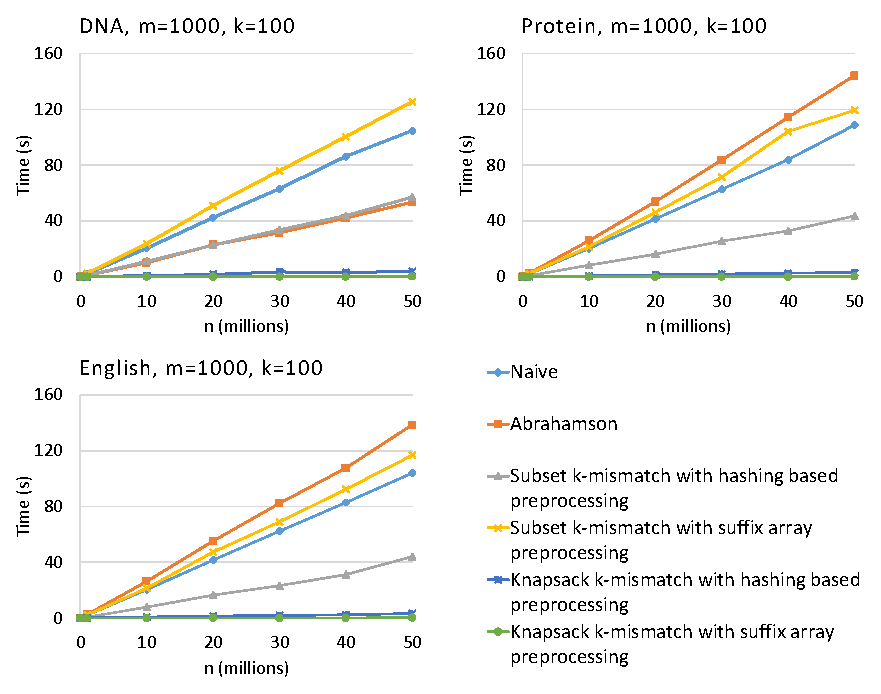
\includegraphics{fig1.eps}

Run times for pattern matching on DNA, protein and
English alphabet data, when the length of the text ($n$) varies.
The length of the pattern is $m=1000$. The maximum number of mismatches
allowed is $k=100$.
Our algorithms are Subset
k-mismatch with hashing based preprocessing (section
\ref{sec_k_mism_det}), Subset k-mismatch with suffix array preprocessing (section \ref{sec_k_mism_det}),
Knapsack k-mismatch with hashing based preprocessing (section
\ref{sec_nsqrtk}), and Knapsack k-mismatch with suffix array preprocessing (section
\ref{sec_nsqrtk}). 
\end{figure*}



\begin{figure*}
\caption{Run times for pattern matching when the length of the pattern
varies.}
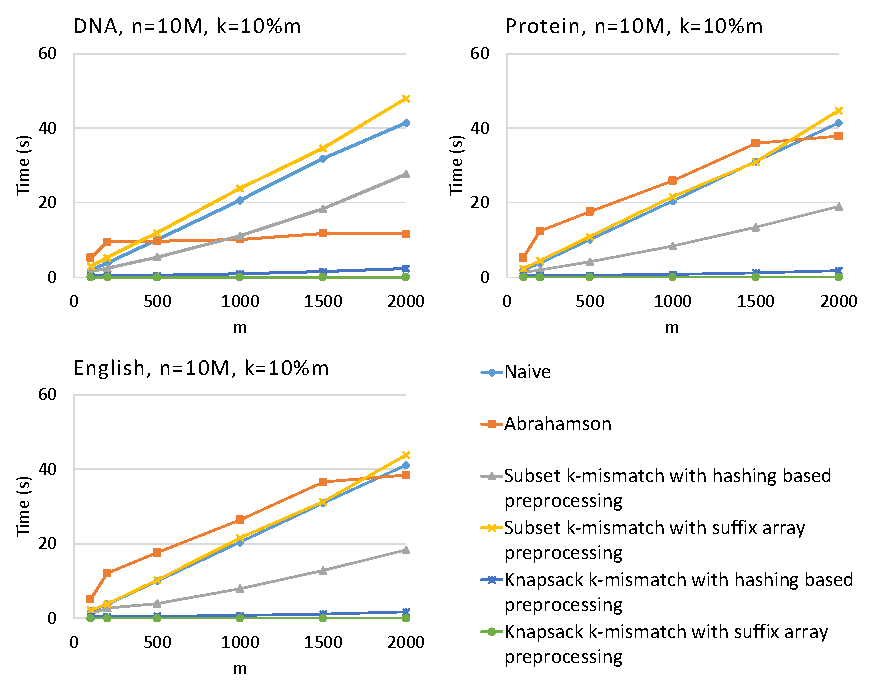
\includegraphics{fig2.eps}

Run times for pattern matching on DNA, protein and
English alphabet data, when the length of the pattern ($m$) varies.
The length of the text is $n = 10$ millions. The maximum number of
mismatches allowed is $k=10\%$ of the pattern length.
Our algorithms are Subset
k-mismatch with hashing based preprocessing (section
\ref{sec_k_mism_det}), Subset k-mismatch with suffix array preprocessing (section \ref{sec_k_mism_det}),
Knapsack k-mismatch with hashing based preprocessing (section
\ref{sec_nsqrtk}), and Knapsack k-mismatch with suffix array preprocessing (section
\ref{sec_nsqrtk}).
\label{fig_runtimes_varym} 
\end{figure*}



\begin{figure*}
\caption{Run times for pattern matching when the maximum number of mismatches
allowed varies.}
\label{fig_runtimes_varyk} 
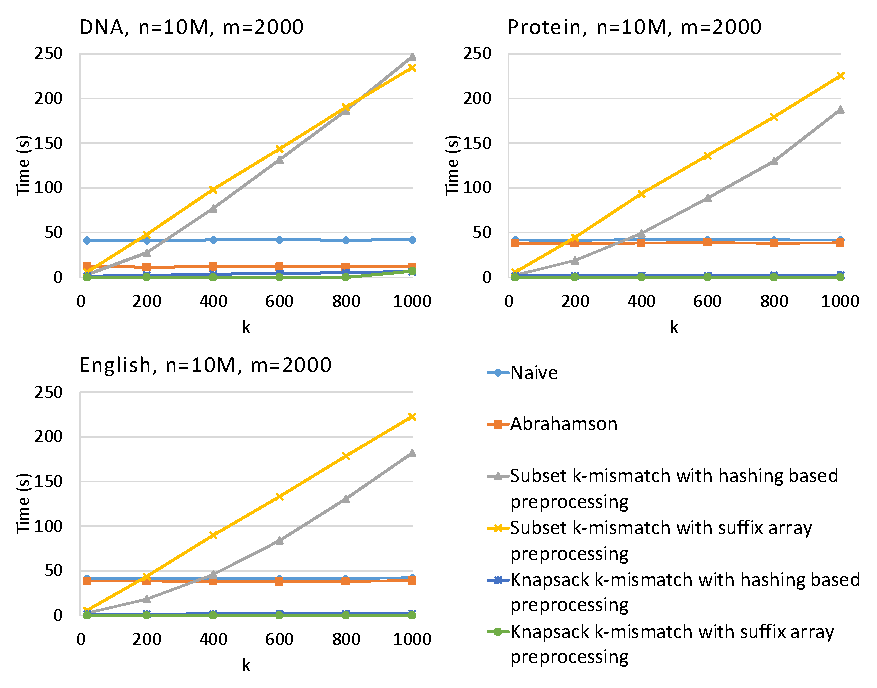
\includegraphics{fig3.eps} 

Run times for pattern matching on DNA, protein and
English alphabet data, when the maximum number of mismatches allowed ($k$)
varies.
The length of the text is $n=10$ millions. The length of the pattern is
$m=2000$.
Our algorithms are Subset
k-mismatch with hashing based preprocessing (section
\ref{sec_k_mism_det}), Subset k-mismatch with suffix array preprocessing (section \ref{sec_k_mism_det}),
Knapsack k-mismatch with hashing based preprocessing (section
\ref{sec_nsqrtk}), and Knapsack k-mismatch with suffix array preprocessing (section
\ref{sec_nsqrtk}). 
\end{figure*}



\begin{figure*}
\caption{Run times for pattern matching when the size of the alphabet varies.}
\label{fig_runtimes_varySigma} 
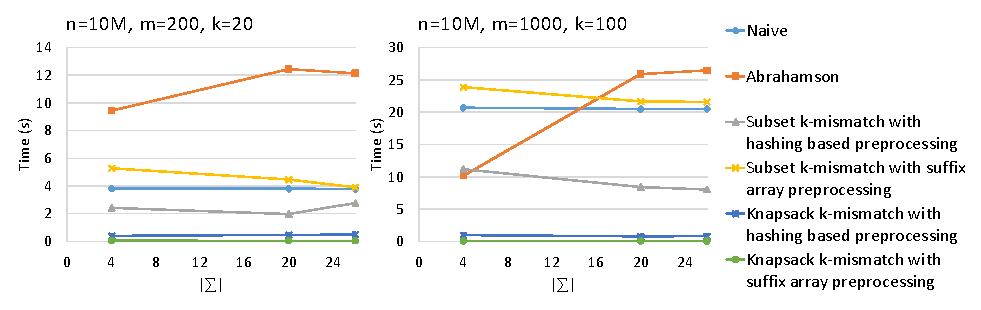
\includegraphics[width=\linewidth]{fig4.eps} 

Run times for pattern matching when the size of the alphabet varies
from 4 (DNA) to 20 (protein) to 26 (English).
The length of the text is $n=10$ millions. The length of the pattern is
$m=200$ in the first graph and $m=1000$ in the second. The maximum number of
mismatches allowed is $k=20$ in the first graph and $k=100$ in the second.
Our algorithms are Subset k-mismatch with hashing based
preprocessing (section \ref{sec_k_mism_det}), Subset k-mismatch with suffix array preprocessing (section \ref{sec_k_mism_det}),
Knapsack k-mismatch with hashing based preprocessing (section
\ref{sec_nsqrtk}), and Knapsack k-mismatch with suffix array preprocessing (section
\ref{sec_nsqrtk}). 
\end{figure*}


\section{Conclusions}
We have  introduced several deterministic and randomized, exact and
approximate algorithms for pattern matching with mismatches and the $k$-mismatches
problems, with or without wild cards. These algorithms improve the run time, 
simplify, or extend previous algorithms wild cards. 
We have also implemented some of the deterministic algorithms. An empirical
comparison of these algorithms showed that the algorithms based on
character comparison outperform those based on convolutions.


\cleardoublepage
\phantomsection
\addcontentsline{toc}{chapter}{Bibliography}
\bibliographystyle{plain}
\bibliography{pms8-references,pms9-references,sa-references,kmis-references,our-references} 


\end{document}
